\documentclass[a4paper, 10pt, openright]{report}
%\documentclass[a4paper, 10pt]{report}
\usepackage[
   a4paper,
   twoside,
   bindingoffset=1.2cm,
   inner=2cm,
   outer=2.5cm,
   top=3cm,
   bottom=3cm,
   headsep=1.2cm
]{geometry}

\usepackage{graphicx}
\usepackage{booktabs}
\usepackage{url}
\usepackage[english]{babel}
\usepackage[latin1]{inputenc}
\usepackage{hyperref}
\hypersetup{
    colorlinks,
    citecolor=black,
    filecolor=black,
    linkcolor=black,
    urlcolor=black
}
\usepackage{mathenv}
\usepackage{amsmath}
\usepackage{mathtools}
\usepackage{color}
\usepackage{caption}
\usepackage[bottom]{footmisc}
\usepackage{cancel}
\usepackage{multirow}
\usepackage[toc,page]{appendix}
\usepackage[]{acronym}
\usepackage{setspace}
%\usepackage[Sonny]{fncychap}
\usepackage{fancyhdr}
\usepackage{titlesec}
\usepackage{gensymb}
\usepackage{emptypage}
\usepackage{fancyhdr}
\usepackage{subfigure}
\usepackage{float}

\makeatletter
\titleformat{\chapter}[block]
  {\Huge}{\filright\enspace \@chapapp~\thechapter\enspace \\}
  {8pt}{\Huge\bfseries\filcenter}
\titlespacing*{\chapter}
  {0pt}{0pt}{50pt}
\makeatother

%\setlength{\headheight}{20pt}
%\pagestyle{fancy}
%\renewcommand{\chaptermark}[1]{\markboth{#1}{#1}}
%\rhead{\thepage \hfill \leftmark}
%\lhead{\thepage \hfill \leftmark}
%\cfoot{}

\begin{document}

\renewcommand{\listfigurename}{List of figures} 
\renewcommand{\listtablename}{List of tables}

%Titlepage
\doublespacing
\baselineskip=0.8\baselineskip
\setlength{\parindent}{0pt}	

\pagenumbering{roman}
\begin{titlepage}

	\centering
	
\includegraphics[width=0.15\textwidth]{figs/image_UC.png}\par
	{\scshape\LARGE Facultad de Ciencias \\ \vspace{-15pt} Universidad de Cantabria \par}
	
	\vspace{0.8cm}
	
	%English title
	\noindent\rule{15cm}{0.4pt}\par 
	{\huge\bfseries Search for dark matter production in association with top quarks in the dilepton final state at $\sqrt{s} = $ 13 TeV\par \vspace{10pt}}
	\noindent\rule{15cm}{0.4pt}\par 
	
	{\vspace{20pt} \Large A thesis submitted in fulfillment of the requirements for the \par \LARGE \textbf{Degree of Doctor of Philosophy} \vspace{20pt} \par \noindent\rule{15cm}{0.4pt}}
	
	\vspace{0.8cm}
	{\Large Written by \\ \textbf{C\'{e}dric Prie\"{e}ls}\par}
	\vspace{0.5cm}
	{\Large Under the supervision of \\ \textbf{J\'{o}natan Piedra G\'{o}mez} \\
	\vspace{-10pt}
	\textbf{Pablo Mart\'{i}nez Ruiz del \'{A}rbol}\\}
	\vspace{1.4cm}
	{\Large Santander, June 2020}
	\vfill

\end{titlepage}

%Empty page

\clearpage
\thispagestyle{empty}
\phantom{a}
\vfill
\newpage

%Abstract and keywords

\setlength{\parskip}{5pt}
\setcounter{page}{1}

\chapter*{\huge{Abstract}}
\newpage
%
\chapter*{\huge{Resumen}}
\newpage
%
\chapter*{\huge{Acknowledgments}}
\newpage
%
\chapter*{\huge{Acronyms used}}
\begin{acronym}

%List all the acronyms used
\acro{SM}[SM]{Standard Model}
\acro{DM}[DM]{Dark Matter}
\acro{LHC}[LHC]{Large Hadron Collider}
\acro{CMS}[CMS]{Compact Muon Solenoid}
\acro{ATLAS}[ATLAS]{A Toroidal LHC ApparatuS}
\acro{CERN}[CERN]{European Council for Nuclear Research}
\acro{QFT}[QFT]{Quantum Field Theory}
\acro{CMB}[CMB]{Cosmic Microwave Background}
\acro{ML}[ML]{Machine Learning}
\acro{MFV}[MFV]{Minimal Flavour Violation}
\acro{WIMP}[WIMP]{Weakly Interactive Massive Particle}
\acro{PF}[PF]{Particle Flow}
\acro{BSM}[BSM]{Beyond the Standard Model}
\acro{MACHO}[MACHO]{Massive Compact Halo Object}
\acro{MSSM}[MSSM]{Minimal Supersymmetric Standard Model}
\acro{SI}[SI]{Spin Independent}
\acro{SD}[SD]{Spin Dependent}
\acro{CL}[CL]{Confidence Level}
\acro{QCD}[QCD]{Quantum ChromoDynamics}
\acro{ADMX}[ADMX]{Axion Dark Matter Experiment}
\acro{CAST}[CAST]{CERN Axion Solar Telescope}
\acro{IAXO}[IAXO]{International Axion Observatory}
\acro{LNGS}[LNGS]{Laboratori Nazionali del Gran Sasso}
\acro{UED}[UED]{Universal Extra Dimensions}
\acro{NFW}[NFW]{Navarro-Frenk-White}
\acro{LAT}[LAT]{Fermi Large Telescope}
\acro{IACT}[IACT]{Imaging Atmospheric Cherenkov Telescopes}
\acro{CTA}[CTA]{Cherenkov Telescope Array}
\acro{AMS}[AMS]{Alpha Magnetic Spectrometer}
\acro{EFT}[EFT]{Effective Field Theory}
\acro{ISR}[ISR]{Initial State Radiation}
\acro{DMWG}[DMWG]{Dark Matter Working Group}
\acro{MET}[MET]{Missing Transverse Energy}
\acro{VBF}[VBF]{Vector Boson Fusion}
\acro{BR}[BR]{Branching Ratio}

\end{acronym}
\newpage

%Table of contents
\tableofcontents

\thispagestyle{empty}
\newpage

%Here it starts!
\setlength{\parskip}{10pt}
\pagenumbering{arabic}

%Introduction

\chapter{Introduction}

The \ac{SM} of particle physics introduced in Section~\ref{section:SM} is nowadays the most accepted mathematical model used to describe the elementary particles and three of the four fundamental forces of nature (electromagnetic, weak and strong interactions). This model is quite simple in concept, but has been able to describe most of the phenomena observed in nature so far with an incredible level of precision, and made a lot of predictions that have now been proven to be true, such as the postulate of the Higgs mechanism \cite{HiggsPostulate1, HiggsPostulate2} followed by the discovery of the Higgs boson itself \cite{HiggsDiscovery1, HiggsDiscovery2} by the \ac{CMS} and \ac{ATLAS} experiments analyzing the proton-proton collisions produced by the \acf{LHC} at a center of mass energy $\sqrt{s} = 13$ TeV, announced at the \ac{CERN} on the 4th of July 2012. 

However, as accurate as it seems to be, this theory is known to have several shortcomings which require further investigation. Eventual exotic particles which do not fit in the current model could be the sign of new physics and have therefore been extensively searched for over the course of the last decades in order to enhance our understanding of the Universe and all its constituents.

In this context, the first serious \ac{DM} hypothesis was introduced in the 1970s because of gravitational anomalies observed by several astrophysicists, as a way to explain the apparent non-luminous missing mass in the Universe \cite{FirstEvidence}. Indeed, the visible mass in most galaxies appears to be way too low to explain several astrophysical processes, such as the rotation curves of the galaxies \cite{RotationCurves}, which seems to be incompatible with the well established laws of gravitation. Some additional measurements of the gravitational lensing (in the Bullet Cluster, for example \cite{BulletCluster}) and the anisotropies observed in the \ac{CMB} \cite{CMBAnisotropies} are other evidences for the existence of \ac{DM}, as explained in Section~\ref{section:DMOrigins}.

As far as we currently know from cosmological measurements, ordinary baryonic matter only constitutes around 5\% of the Universe, while  \ac{DM} represents around 26\% of the energy density of the Universe (the rest is being considered as dark energy) \cite{Repartition}. Understanding the nature and properties of this new kind of exotic matter is therefore crucial to try and understand the physics in the Universe, with many large experiments around the world currently involved in such searches. 

Nowadays, the existence of \ac{DM} is well established in the physics community, even though it has never been observed directly, since our only evidences so far for its existence come from its large-scale gravitational effects. While its mass, spin, nature and basic properties are still unknown and extensively studied, one of the best \ac{DM} candidate is the so-called \ac{WIMP}, predicted to interact both gravitationally and weakly with \ac{SM} particles. This would allow direct and indirect direction of such candidates, used as the driving process of many of experiments over the last decades, trying to find the hint of a possible interaction between standard baryonic particles and eventual \ac{DM} particles, or even between several \ac{DM} particles themselves. Dark matter production through the use of a particle accelerator colliding \ac{SM} particles together, such as the \ac{LHC}, is also a possibility, and will be consider as the main channel towards the eventual detection of this exotic matter throughout this work. The production through colliders is actually able to provide constraints on low dark matter masses as well, in a region where both the direct and indirect searches are less efficient, which makes the \ac{LHC} a perfect tool to study this kind of \ac{BSM} physics. These searches will be summarized in Section~\ref{section:DMSearches}.

However, observing \ac{DM} is still extremely difficult, mainly because it barely interacts with ordinary baryonic matter, except through gravity (we have to assume that it does interact with \ac{SM} at least weakly for the sake of this work though, as we would not be able to discover it as an individual particle if it were not the case). This means that nowadays, all the experiments searching for \ac{DM} have only been able to put constraints on the \ac{DM} particle mass and on the interaction cross sections between the dark and standard sectors. Actually, even if the collisions between protons produced by the LHC do have a sufficient amount of energy to produce this kind of particles, we would not expect them to interact with our detector, making their detection even harder. The eventual presence of such matter has to be inferred from the study of the interaction between \ac{SM} particles and \ac{CMS} itself, since a typical \ac{DM}-like event consists of at least one energetic \ac{SM} particle produced in association with a large imbalance in the transverse momentum due to the presence of an eventual \ac{DM} candidate that was able to escape our detection. %This kind of collider searches can be grouped under the name of \textit{mono-X} searches, where the \textit{X} stands for any kind of \ac{SM} particle (a jet, a lepton or a photon for example). 

In the context of this work, \ac{DM} is searched for in association with one or two top quarks which play the role of the \ac{SM} particle allowing us to trigger the event. This is indeed a perfect channel for this kind of searches if we assume that the interaction between the dark and standard sectors respect the principle of \ac{MFV}, which can be consistently defined independently of the structure of the new physics model \cite{MFVYukawa}. In this case, this interaction should follow the same Higgs-like Yukawa coupling structure as the usual \ac{SM} baryonic particles, which actually depend on the mass: the heavier the \ac{SM} particle considered is, the easier it is for it to couple with the dark sector. This makes the top quark, the most massive of all the fundamental particles observed by far, an excellent object to study in this context.

However, this also means that the phenomenology of this quark is mostly driven by its large mass and that it decays before hadronization can occur, usually into a W boson and and a bottom quark. The final state of the process we are interested in is then be made of some b jets, leptons and/or quarks and is categorized depending on this number of b-tagged jets and on the decay of the W itself. This work will actually be focused on the two leptons final state, also known as the dileptonic channel, mostly since this channel does not have lots of background processes raising to a similar final state, even though its branching ratio is the smallest, as will be explained in Section~\ref{section:ourChannel}. Additionally, leptons are by reconstruction much cleaner than jets: their identification and momentum calculation is easier to perform, and the uncertainties associated to these measurements will be smaller.

The \ac{LHC} has now been running for 10 years, and several similar searches have already been carried out and published in the past by the \ac{CMS} and \ac{ATLAS} collaborations, at different center of mass energies. First of all, at 8 TeV, several searches for a pair of top quarks were published by the \ac{CMS} (in association with \ac{DM} in the semileptonic \cite{PreviousDoubleTopSingleLep8CMS} and dileptonic \cite{PreviousDoubleTopDiLep8CMS} final states) and \ac{ATLAS} collaborations \cite{PreviousDoubleTopAllLep8ATLAS}. Then, at 13 TeV, the \ac{ATLAS} collaboration published on one hand several studies, considering different final states and different luminosities (13.3 fb$^{-1}$ and 36.1 fb$^{-1}$) \cite{PreviousDoubleTopNoLep13ATLAS, PreviousDoubleTopOneLep13ATLAS, PreviousDoubleTopDiLep13ATLAS}. On the other hand, the \ac{CMS} collaboration published a few extremely important papers for this study \cite{PreviousDoubleTopBottomAllLep13CMS, PreviousDoubleTopAllLep13CMS}. For the first time in 2019, the results obtained by the $t/\bar t$+DM and $t \bar t$+DM analyses have also been combined and published using the 2016 data \cite{PreviousSingleDoubleTopAllLep13CMS}. Our main objective is now to repeat and improve this analysis while considering the full Run II dataset, globally improving the analysis strategy and including the dileptonic final state for the first time in this combination.

After a general introduction about \ac{DM} in general in Chapter~\ref{chapter:Case}, the experimental device will be detailed in the Chapter~\ref{chapter:Device}. This will include a discussion about the \ac{LHC} itself, along with a complete description of \ac{CMS}, the detector used to collect the data that will be analyzed throughout this work. This data has been collected during the years 2016, 2017 and 2018 and corresponds to an integrated luminosity of $\sim 138$ fb$^{-1}$, collected during the Run II of operation of the \ac{LHC} and at a center of mass energy $\sqrt{s} = 13$ TeV. In particular, a particular care will be given to the explanation of the \ac{PF} algorithm, used to reconstruct the different objects used and that will be defined in the Chapter~\ref{chapter:Reco}, while the estimation of the different backgrounds and the selection of interesting events will be detailed throughout the Chapters~\ref{chapter:Samples} and~\ref{chapter:Selection}.

Distinguishing between the signal we are searching for and backgrounds having a much higher cross-section and kinematically really close, such as the \ac{SM} $t \bar t$ without production of \ac{DM} is not a straightforward task (sometimes a production of missing transverse energy due to the presence of physical neutrinos is even obtained). To isolate the signal and to obtain some discrimination between these kind of processes, an algebraic reconstruction of the event and top-notch \ac{ML} techniques are used in this work, in order to train a network of neurons to perform this task. The main objective is to make them learn how to combine the discriminating power of a set of input variables in order to create a single output variable describing the probability of a single event to be classified as signal or background. All this process will be detailed in Section~\ref{section:Discrimination}.

Finally, a statistical interpretation of our data will be performed and different sources of systematic uncertainties will be considered in Chapter~\ref{chapter:FinalResults}. This will allow us to set upper limits on the cross section production value of \ac{DM} particles in our particular channel and for the simplified models considered in this analysis. The conclusions of this work and some additional future prospects will then finally be presented in Chapter~\ref{chapter:Conclusion}.
\\

%Empty page

%\clearpage
%\thispagestyle{empty}
%\phantom{a}
%\vfill
%\newpage

\chapter{The Dark Matter case}\label{chapter:Case}

In this chapter, some general explanations about the \acf{SM} will first of all be given in Section~\ref{section:SM} as a general introduction about today's most accepted mathematical model describing all the known particles and their interactions. The case for \acf{DM} will then be presented in Section~\ref{section:DMOrigins}, along with a summary of the main evidences, mostly astrophysical, which lead to the introduction of this kind of \acf{BSM} physics. Then, the main properties expected by such exotic matter will be introduced in Section~\ref{section:DMProperties} and nowadays's most accepted \ac{DM} candidates, such as the \acf{WIMP} briefly introduced previously will be presented in Section~\ref{section:DMCandidates}. 

The main ways we have to search (direct, indirect and collider searches) for this new exotic physics along with the main experiments dedicated to such searches will then be shown in Section~\ref{section:DMSearches}. Finally, the searches performed in colliders such as the \acf{LHC} and our particular channels of interest (\ac{DM} produced in association with either one or two top quarks) will be detailed in Section~\ref{section:ourChannel} and the latest similar results and exclusion plots published over the course of the previous years by the \ac{ATLAS} and \ac{CMS} collaborations will be shown in Section~\ref{section:PreviousResults}.

\section{The \acf{SM}} \label{section:SM}

The \acf{SM} of particle physics is a relativistic \ac{QFT} theory which is able to  mathematically summarize our current understanding of all the particles surrounding us and to describe three out of the four main interactions between these particles (mainly the weak, strong and electromagnetic forces, while an explanation of the origin of the gravitational interaction is still out of the reach of this theory nowadays). 

If the neutrinos are considered to be normal Dirac fermions (and the question whether or not they could actually be Majorana particles is still well under discussion \cite{Majorana}), then the \ac{SM} contains 26 free parameters, mainly the masses of the 12 predicted fermions, as shown in Figure~\ref{figure:SMFermions}, along with the couplings describing the strengths of the three interactions, two parameters describing the Higgs potential, eight mixing angles and, maybe, the phase of the eventual strong CP violation that we will mention in Section~\ref{section:DMCandidates} (but in any case this parameter is expected to be close to 0). This is a quite high number of free parameters, but the value of most of them has now been derived experimentally, to match the observations made over the last decades.

\begin{figure}[htbp]
\begin{center}
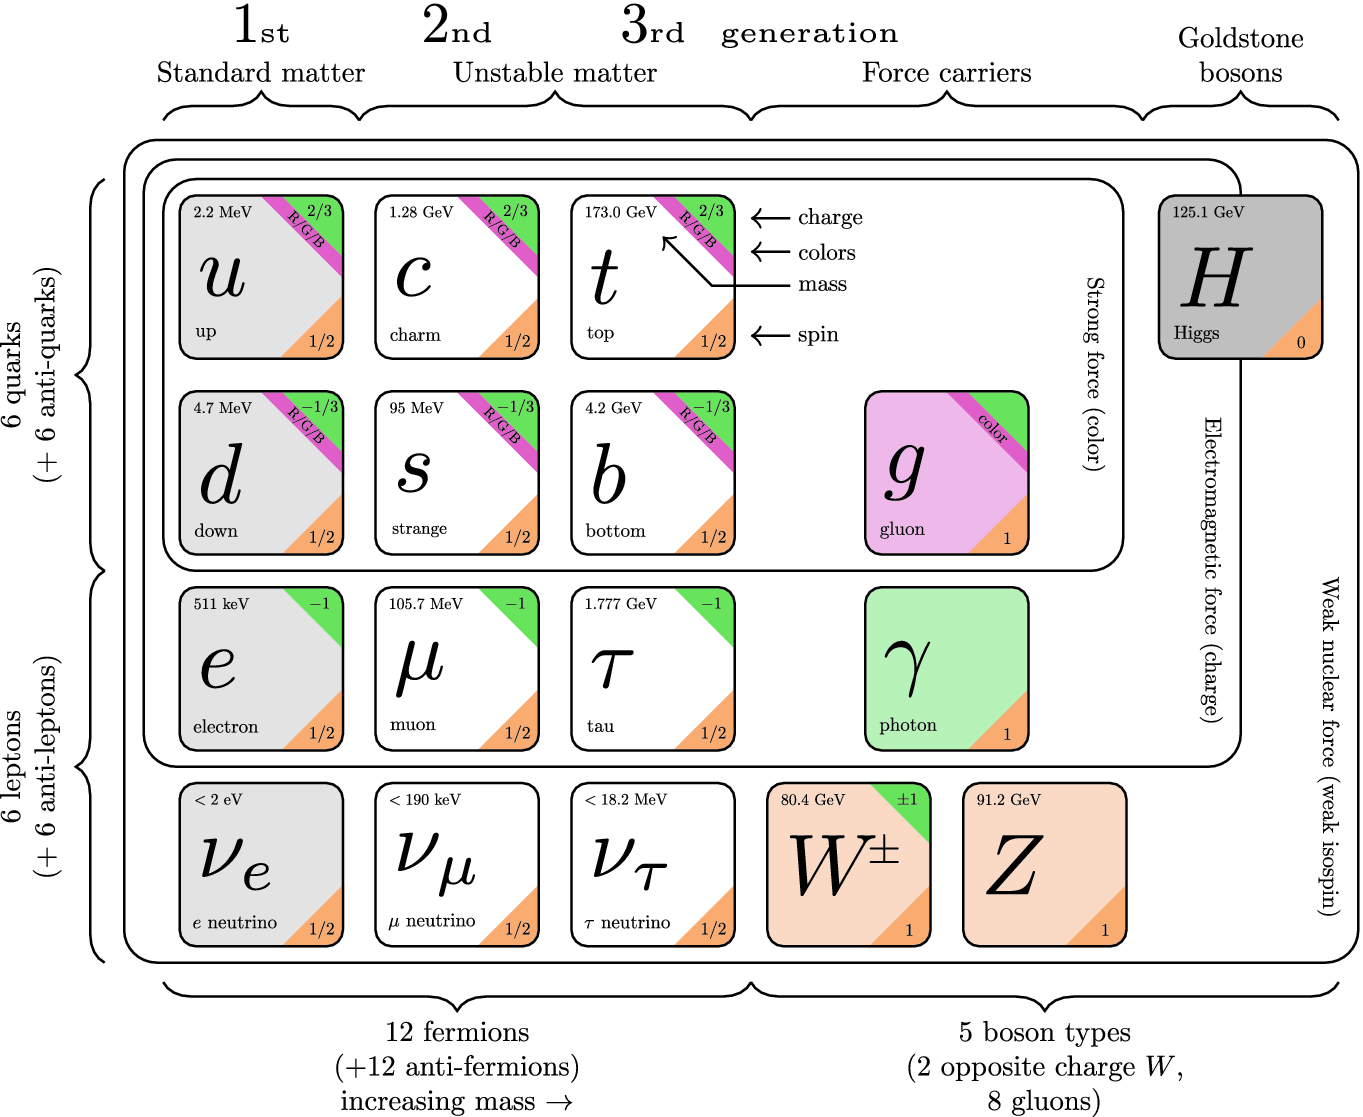
\includegraphics[width=8cm, height=6cm]{figs/SMFermions.png}
\caption{Representation of the 12 fermions of the \ac{SM} \cite{SMFermions}.}
\label{figure:SMFermions}
\end{center}
\end{figure}

The \ac{SM} Lagrangian density in a differential volume element $\mathcal{L} = \int L \text{ } d^3x$, accounting for the kinetic and potential energy of a system, takes the (very) simplified form given by Equation~\ref{eq:SMLag}, where the $F_{\mu \nu}$ is the field strength tensor accounting for the different interactions, $\psi$ is the interacting field describing quarks and leptons and $\phi$ is the Brout-Englert-Higgs field while $y_{ij}$ are the Yuwaka couplings to this field, which depend on the mass of the particle considered and which will be described later on in Section~\ref{subsection:ColliderProduction}.

\begin{equation}
\mathcal{L} = - \frac{1}{4} F_{\mu \nu} F^{\mu \nu} + i \bar{\psi} \cancel{D} \psi + \bar{\psi}_i y_{ij} \psi_j \phi + |D_\mu \phi|^2 - V(\phi)
\label{eq:SMLag}
\end{equation}

A complete description of this model is unfortunately out of the scope of this work but it is important to note that the \ac{SM}, although mostly experimental, is still working extremely well today. Indeed, it managed to make a lot of predictions over the years, which is the best you can obtain from a mathematical model, and most of its predictions revealed themselves to be true (we can quote for example that it successfully predicted the existence of the gluons, the top quarks, along with the W, Z and Higgs bosons \cite{SMPredictions}).

However, even though it now appears to be complete since all its predictions have been discovered, we know that the \ac{SM} is not the final theory of particle physics since it is not able to explain all the observations which have been made. There are still today some open questions and many \acf{BSM} theories trying to explain such observations which do not fit inside the \ac{SM}, such as an eventual inclusion of the gravitational interaction within this model. We can quote for example as successful \ac{BSM} theories the possible existence of the supersymmetry, telling us that each particle should have a superpartner whose spin differs by 1/2 or the possible existence of \acf{DM} particles, the main subject of the discussion of the following sections.

\section{At the origins of dark matter} \label{section:DMOrigins}

The origin of the concept of dark matter can be traced back to the 17 and 18th centuries, shortly after Newton's works on gravitation, even though this concept changed quite a lot over the years. Back then, \ac{DM} was more considered to be ordinary matter which simply did not emit any kind of electromagnetic radiation, being therefore invisible and dark, but which does have a strong impact in the gravitational point of view because of its mass. It was for example considered in the 20th century to be found in massive astronomical objects able to absorb the light or other objects located behind them, such as black holes (and even some actual theories still believe this is true!).

\subsection{Zwicky and the virial theorem}

In the 20th century, the first experimental evidences for the existence of dark matter were shown. In 1933, Fritz Zwicky managed to determine the mass of the Coma Cluster using the virial theorem \cite{Zwicky}, which states that in a cluster in equilibrium under its own gravitation the kinetic energy must be comparable to its gravitational binding energy. 

Mathematically, the virial theorem can be written in Equation~\ref{equation:Virial}, where the brackets represent the mean value of the quantity obtained over time or position, the universal constants of gravitation is $G = 6.67 \cdot 10^{-11}$ m$^3$ kg$^{-1}$ s$^{-2}$ and where the gravitation potential energy expression can be simplified assuming a spherical distribution of the masses and the same average density everywhere in the cluster considered.

\begin{equation} \label{equation:Virial}
2 \langle T \rangle + \langle V \rangle = 0 \text{, where}
\begin{dcases}
T = \frac{1}{2} \sum_i M_i v_i^2 = \frac{1}{2} M \langle v^2 \rangle\\
V = -4 \pi G \int_0^R M \rho \text{ } r \text{ } dr \propto \frac{G M^2}{R}
\end{dcases}
\end{equation}

Solving these simple equations gives us an approximate value of the mass of the cluster in Equation~\ref{equation:ClusterMass}, where R is the radius of the cluster and $\langle \langle v^2 \rangle \rangle$ is the squared velocity of all the galaxies averaged over position and time.

\begin{equation} \label{equation:ClusterMass}
M \propto \frac{\langle \langle v^2 \rangle \rangle R}{G}
\end{equation} 

From this simple expression and astronomical observations, Zwicky then managed to compute the average mass to light ratio of its galaxies and concluded that the value obtained was around 400-500 times larger than the mass previously estimated by Edwin Hubble, who simply considered the number of visible galaxies within this cluster for his calculations. One plausible explanation for this discrepancy is to introduce the concept of \ac{DM}, which contributes to the mass of the cluster without increasing the galactic luminosity.

Zwicky's results were actually quite controversial since they were based on statistical calculations relying on different hypotheses not always justified, such as the fact that the galaxies in the cluster must be gravitationally bound with each other and they were actually proven to be overestimated later on \cite{ZwickyWrong}, but additional observations came to enforce to validity of his conclusions anyway.

\subsection{Spiral galaxies rotation curves}

Despite being controversial and slightly off, Zwicky's results were soon followed by a series of additional astronomical observations leading to the same conclusion, the possible existence of non-luminous matter in all the galaxies, called dark matter. The most famous of these results is the study of the observed and expected rotation curves of the stars within spiral galaxies such as the Milky Way in the 1970s \cite{RotationCurves}. 

According to this study, if we assume that we can apply Newton's universal laws of gravitation at the galactic scale, then the stars within this kind of galaxies should rotate with a velocity depending on the radius to the galactic center obtained by the usual equation for centripetal acceleration in a gravitational field and represented in Equation~\ref{equation:RotationVelocity}, where $M(r)$ accounts for the total mass encountered in a radius $r$.

\begin{equation} \label{equation:RotationVelocity}
v_{\text{rotation}}(r) = \sqrt{\frac{G M(r)}{r}}
\end{equation}

At first approximation, one can assume that most of the mass within this kind of galaxies comes from the inner core, which means that, at large radius, the velocity of individual stars is expected to decrease proportionally to $r^{-1/2}$. Any deviation to this rule suggest that either our understanding of gravity at large scales or our basic understanding of galaxies as a celestial body made of stars, dust and gas, has to be revised.

Actually, observations made by Vera Rubin and her team in the early 1970s with a new spectrograph designed to study the velocity curves of spiral galaxies with a degree of accuracy never reached before, did not confirm these expectations \cite{VeraRubin}. Indeed, according to these results, from a given value of the radius, the velocity curve appears to be flat instead of decreasing, as illustrated in Figure~\ref{figure:RotationCurves}. This is another hint that can motivate the introduction of the concept of \ac{DM}.

\begin{figure}[htbp]
\begin{center}
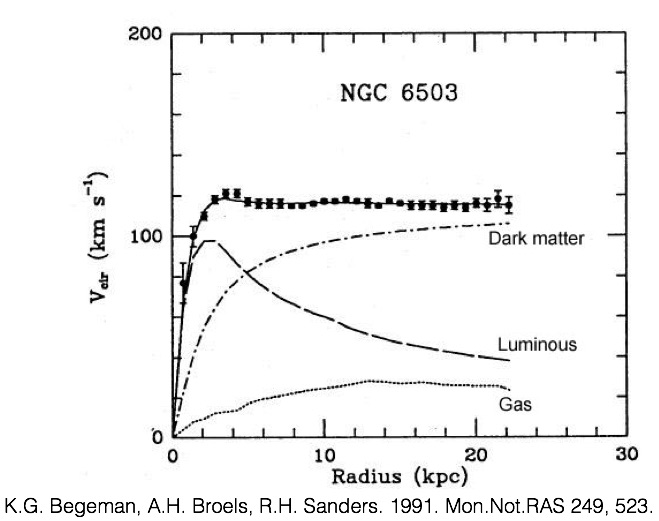
\includegraphics[width=8cm, height=6cm]{figs/RotationCurve.jpeg}
\caption{Expected and observed rotation curves of the galaxy NGC 6503 \cite{RotationCurves}. The black dots correspond to the data and the \textit{luminous} line corresponds to the expected rotation curve decreasing as $r^{-1/2}$, as expected from Newtonian dynamics.}
\label{figure:RotationCurves}
\end{center}
\end{figure}

\vspace{-10pt}
\subsection{\acf{CMB} anisotropies} \label{subsection:CMB}

The \ac{CMB} is a mostly uniform background of primary radio waves emitted when the Universe became transparent around 380.000 years after the Big Bang and was discovered accidentally in the 1940s \cite{CMBDiscovery}. Studying it is extremely important, as it is actually made of the oldest and cleanest electromagnetic radiation we can find in the Universe. Precise measurements of this radiation are actually critical in many different fields of physics, since any proposed model of the Universe must be able to explain this radiation, its temperature and anisotropies. 

Recent measurements determined that the \ac{CMB} can be considered as emitting a thermal black body spectrum at a temperature of $(2.72548\pm 0.00057)$K \cite{CMBTemperature}. However, we now know that this temperature is actually not constant as some small anisotropies (at the $10^{-5}$ level) depending on the value of the angular angle of observation can be observed, as represented on Figure~\ref{figure:PlanckTemperature}.

\begin{figure}[htbp]
\begin{center}
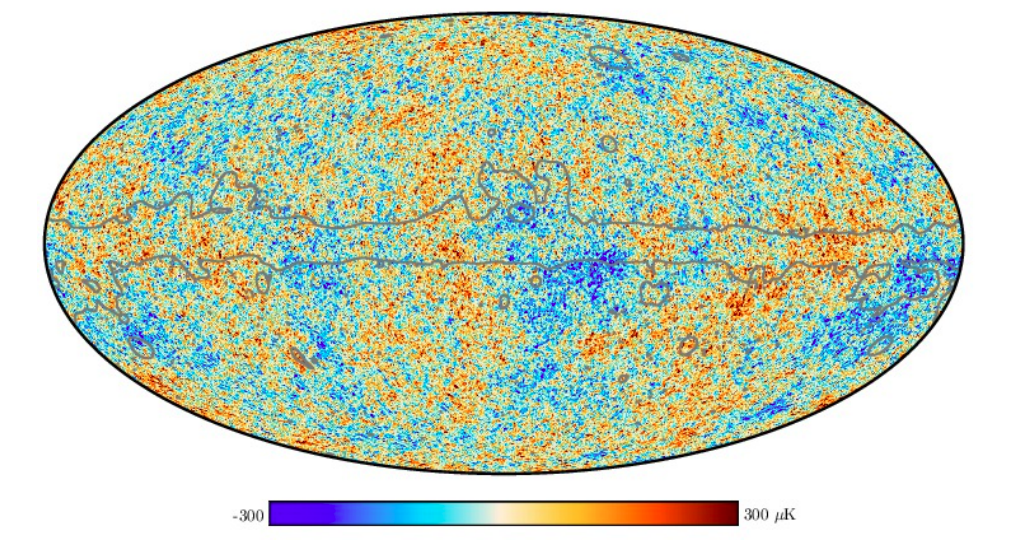
\includegraphics[width=14cm, height=6cm]{figs/PlanckTemperature.png}
\caption{Anisotropies at the $10^{-5}$ level in the temperature of the \ac{CMB}, as observed by the Planck satellite in 2018 \cite{PlanckTemperature}.}
\label{figure:PlanckTemperature}
\end{center}
\end{figure}


We see these fluctuations projected over a 2D sphere, and it is therefore natural to introduce at this point Laplace's spherical harmonics, $Y_{lm} (\theta, \phi)$, a complete set of orthogonal functions obtained by solving Laplace's equation $\nabla \psi = 0$ on a sphere and defined by a few parameters such as $l$, the multipole, representing a given angular angle in the sky (l=100 corresponds to $\sim 1\degree$) and $m$, the number of poles, such as $-l \leq m \leq l$ \cite{PowerSpectrum}. 

It is possible to show that these spherical harmonics form a complete orthonormal basis on this space and therefore that any function can be defined on the sphere may be expanded into these harmonics using coefficients called $a_{lm}$. The temperature fluctuations, whose value depend on the two usual spherical angles $\theta$ and $\phi$ can therefore be expanded using these generic functions, according to Equation~\ref{equation:SphericalHarmonics}.

\begin{equation} \label{equation:SphericalHarmonics}
\frac{\Delta T}{T}(\theta, \phi) = \sum_{l=0}^{\infty} \sum_{m=-l}^{m=l} a_{lm} Y_{lm} (\theta, \phi)
\end{equation}

The information about the anisotropies can actually be extracted from the variance of these harmonic coefficients $a_{lm}$ of the expansion since the \ac{CMB} is assumed to be a gaussian random field. The power spectrum of the \ac{CMB} can therefore be extracted according to Equation~\ref{equation:PowerSpectrum}, and from which most of the cosmological information of the \ac{CMB} is derived.

\begin{equation} \label{equation:PowerSpectrum}
D_l = \frac{l(l-1) C_l} {2\pi} = \sum_m |a_{lm}^2|
\end{equation}

Interestingly enough, this spectrum is directly affected by the value of the density of the dark matter in the Universe, and this is something that will be often discussed in the remaining of this chapter. Doing a multi-parameters fit on the observed data represented in the power spectrum (cf. Figure~\ref{figure:CMBSpectrum}) is then able to give us directly the energy density of baryonic $\Omega_b$ and dark $\Omega_\chi$ matter, along with other important parameters of the $\Lambda CDM$ cosmological model. Today's most precise measurements have been obtained in 2018 using the Plank satellite, and lead to the determination of these two quantities: $\Omega_b h^2 = 0.02220 \pm 0.00020$ and $\Omega_\chi h^2 = 0.1185 \pm 0.0015$ \cite{Planck}. This is one of the strongest constraint we have on \ac{DM} so far, since any \ac{DM} candidate will need to comply with this measurement.

By dividing these results with the value of the scaling factor for Hubble expansion rate $h = 0.674$ \cite{Constants}, we can obtain from these numbers a proportion of 4.9\% of ordinary baryonic matter and 26.1\% of dark matter in the Universe, as announced in the introduction.

\begin{figure}[htbp]
\begin{center}
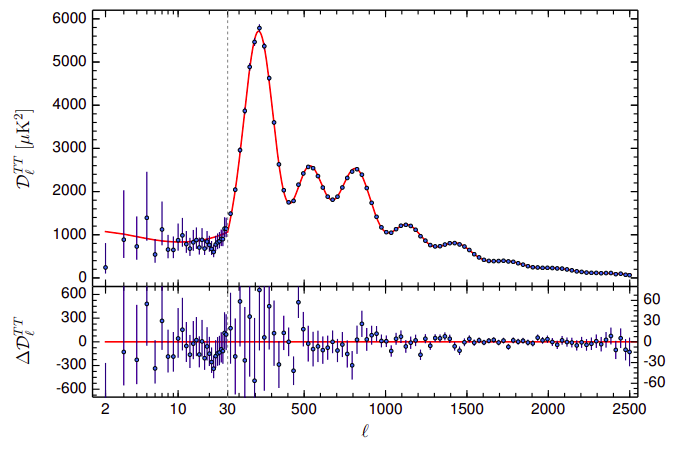
\includegraphics[width=10cm, height=6cm]{figs/PlanckSpectrum.png}
\caption{Power spectrum of the \ac{CMB} obtained by Planck, representing the fluctuations of the temperature of the radiation with respect to the angular angle of observation \cite{Planck}.}
\label{figure:CMBSpectrum}
\end{center}
\end{figure}

\subsection{Gravitational lensing}

The last evidence supporting the existence of dark matter has been obtained by observing several clusters of galaxies in the Universe, such as the Bullet Cluster, and by studying their mass distribution through gravitational lensing.

The gravitational lensing effect is a consequence of the general relativity, a theory developed by Einstein as a way to represent gravity using the geometry of spacetime, stating that massive objects lying between distant sources and an observer should act as a lens and bend the light emitted by the source. This deviation of the light is actually proportional to the mass of the object in between the source and the observer, meaning that the gravitational lensing can give us a way to measure the mass distribution of massive objects, such as galaxy clusters. This mass distribution can then be compared to the luminous distribution of the cluster, to see if we can observe a discrepancy between the two measurements, which could be another hint of the existence of \ac{DM}.

The bullet Cluster is particularly interesting in this context since it actually provides an evidence for the eventual existence of \ac{DM} which does not rely on any mathematical assumption (other than the general relativity principle) and cannot at principle be explained by alternate laws of gravitation. In this case, some observations clearly showed that the spatial deviations between the center of the total mass and the center of the baryonic luminous mass cannot be explained with an alteration of the gravitational force law alone, with a statistical significance of $8 \sigma$ \cite{BulletClusterSigma}.

\begin{figure}[htbp]
\begin{center}
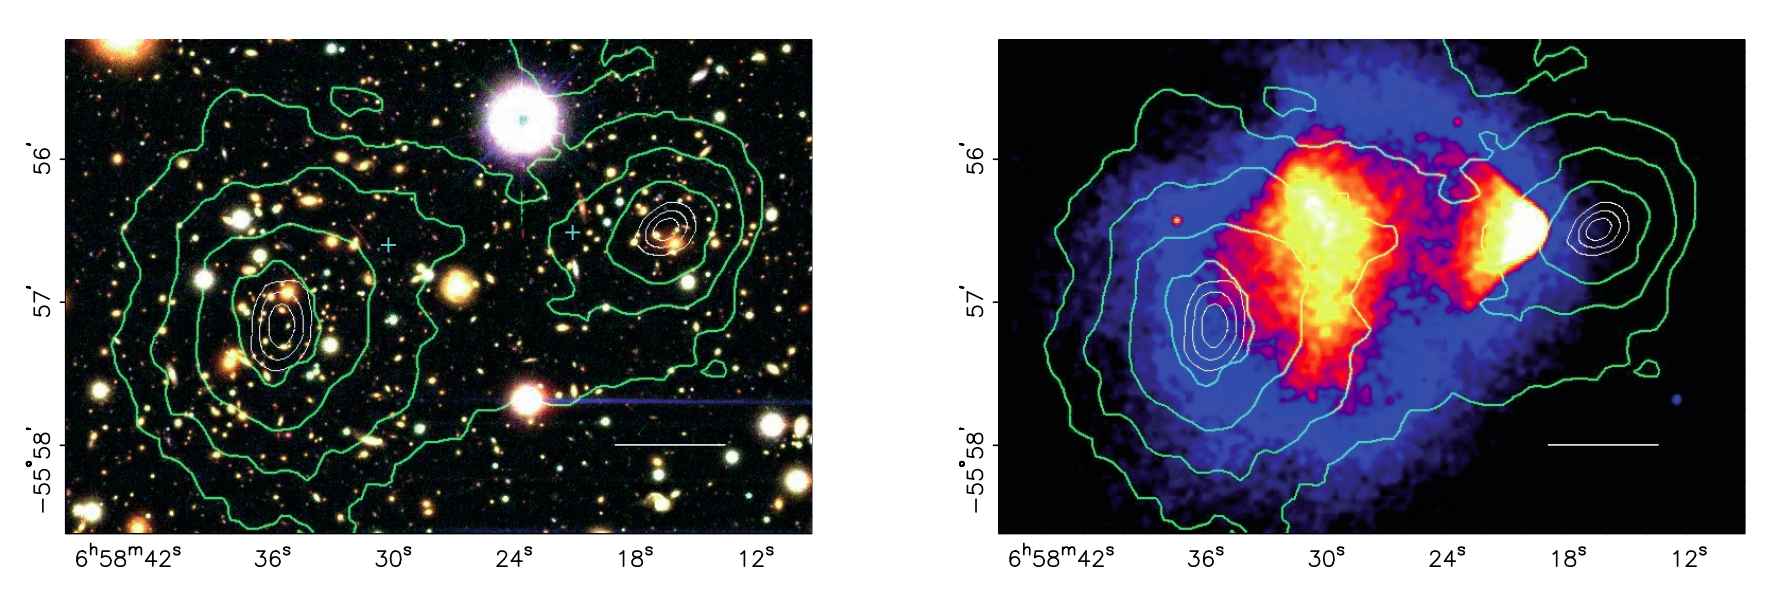
\includegraphics[width=14cm, height=6cm]{figs/BulletCluster.png}
\caption{Mass distributions obtained by the Magellan in the visible (on the left) and Chandra on the X-rays spectrum (on the right) telescopes of the Bullet Cluser. Being shifted compared to each other, this is yet another clear evidence for the existence of \ac{DM} \cite{BulletClusterSigma}.}
\label{figure:BulletCluster}
\end{center}
\end{figure}

As seen in Figure~\ref{figure:BulletCluster}, the image taken by Chandra clearly shows an offset between the visible plasma of the cluster and the actual mass distribution measured through gravitational lensing (green contours). The center of the luminous mass of the cluster does not seem to match the one obtained considering its non-luminous counterpart as well, which is another evidence of the possible existence of \ac{DM} within galaxy clusters.

\section{Dark matter properties} \label{section:DMProperties}

All the previous observations allow us to list some of the most important properties that the perfect dark matter candidate should have. Even though several theories exist, each giving slightly different properties to the \ac{DM}, we will consider in this work the following mostly accepted properties for such particles:
\begin{itemize}
\item First of all, we will assume that \ac{DM} is a \textbf{particle}. As far as we know, the Universe is simply composed of particles so there is no objective reason to think that \ac{DM}, being matter with a certain mass, might not be made of some kind of indivisible particles at some level.
\item Then, the perfect \ac{DM} candidate should of course be \textbf{dark}. This means that it should not interact at all in with electromagnetic radiation such as light, and that it should therefore be \textbf{electrically neutral}. However, it has to interact at least gravitationally because of the evidences for the evidence of such a particle explained before, mostly relying on gravitational effects, and we have to assume in this work that it interacts weakly as well to have a chance to discover it within particle accelerators.
\item It has to be \textbf{non-baryonic}, mainly because the energy density for the baryonic matter obtained by observing the power spectrum of the \ac{CMB} is too low to account for \ac{DM} as well, as explained in Section~\ref{subsection:CMB}. Indeed, according to these results, baryonic matter account for around 5\% while dark matter accounts for more than 25\% of the energy density of the Universe. 
\item We will also only consider \textbf{cold} dark matter, since the widely accepted $\Lambda CDM$ cosmological model is actually based on this assumption. By cold, we do not refer to the temperature of these particles but actually to their size, and therefore to the velocity by which they can travel in the Universe. Large scale structures of the Universe such as we can observe them today cannot actually not be explained if \ac{DM} is made of hot/relativistic particles, as represented in Figure~\ref{figure:ColdWarmDM}. However, although not really as popular, it is important to note that alternative models with warm \ac{DM} have also been developed and still exist today.
\item It is interesting to report as well that \ac{DM} particles are expected to be found near the electroweak symmetry breaking scale, between \textbf{10 GeV and 1 TeV}. This is a consequence of the expected production mechanism of such particles, the so-called thermal freeze-out. 

This principle tells us that at some point in the history, \ac{DM} was supposed to be in thermal equilibrium with other primordial \ac{SM} particles, meaning that its production and annihilation rates were equal, as shown in Equation~\ref{equation:equilibrium}.

\begin{equation}
\label{equation:equilibrium}
\chi \bar \chi \leftrightarrow e^+ e^-, \mu^+ \mu^-, q \bar q, W^+ W^-, ZZ
\end{equation}

However, because of the expansion of the Universe, at some point \ac{DM} particles were simply too far apart from each other and these reactions maintaining this equilibrium were not efficient enough any more. At this stage, the abundance of \ac{DM} became fixed: this is the freeze-out, as represented in Figure~\ref{figure:FreezeOut}.

This principle is interesting because, as a rule of thumb, we can say that if a particle interacts heavily, it will stay longer in equilibrium and its freeze-out abundance will therefore be smaller, so there is a mathematical relation between the strength of the \ac{SM}/\ac{DM} interaction $g$, the mass of the \ac{DM} particle $m_\chi$ and its relic abundance $\Omega_\chi$ that has been precisely measured, as expressed in Equation~\ref{equation:FreezeOut} \cite{FreezeOut}.

\begin{equation}
\label{equation:FreezeOut}
\Omega_\chi \propto \frac{m_\chi^2}{g^4}
\end{equation}

By using a typical value for $g$ of the order of the Fermi coupling constant $G_0^F \simeq 4.54 \cdot 10^14$ J$^{-2}$ we can see that, in order to observe a freeze-out abundance comparable to the one observed recently by the Planck satellite, the \ac{DM} candidate should have a mass between 10 GeV and 1 TeV as previously stated. The measurement of the \ac{CMS} power spectrum is therefore able to put constraints on the \ac{DM} cross-section with the baryonic sector, and all the \ac{DM} candidates quoted in Section~\ref{section:DMCandidates} will have to respect this criteria.

In any case, \ac{DM} is not expected to have a mass lower than 300 eV since at this scale, the phase space density that would be needed to explain this relic abundance of \ac{DM} would simply violate the Pauli-exclusion principle \cite{keVSterile}.

\item Finally, the \ac{DM} particles should be \textbf{long-lived}. Indeed, we expect that they were produced 13.8 billion years ago during the Big Bang, but it seems they are still present in the Universe since we still see their effect today. They should then be stable particles, or their lifetime should at least be larger than the age of the Universe itself.
\end{itemize}

\begin{figure}[htbp]
\begin{center}
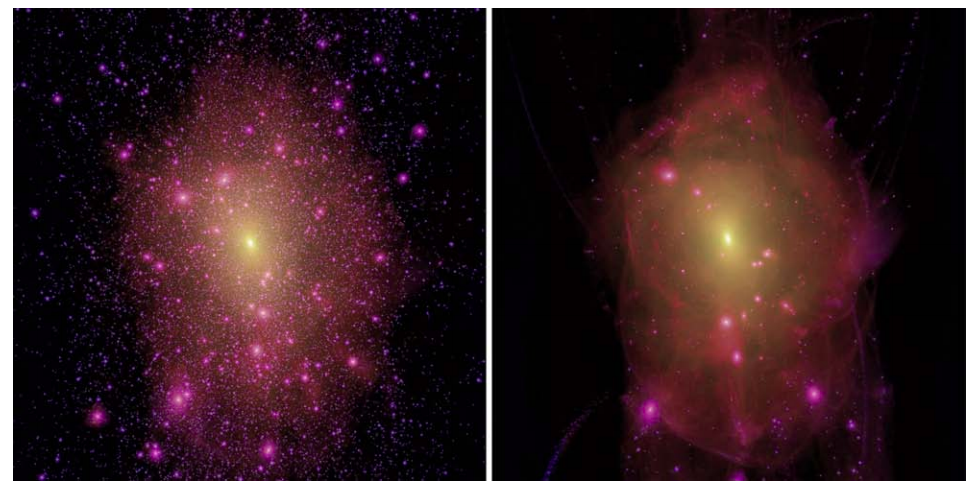
\includegraphics[width=14cm, height=6cm]{figs/ColdWarmDM.png}
\caption{Computer simulations for cold (on the left) and warm (on the right) \ac{DM} scenarios and their impact on a galactic halo at 0 redshift \cite{ColdWarmDM}.}
\label{figure:ColdWarmDM}
\end{center}
\end{figure}

\begin{figure}[htbp]
\begin{center}
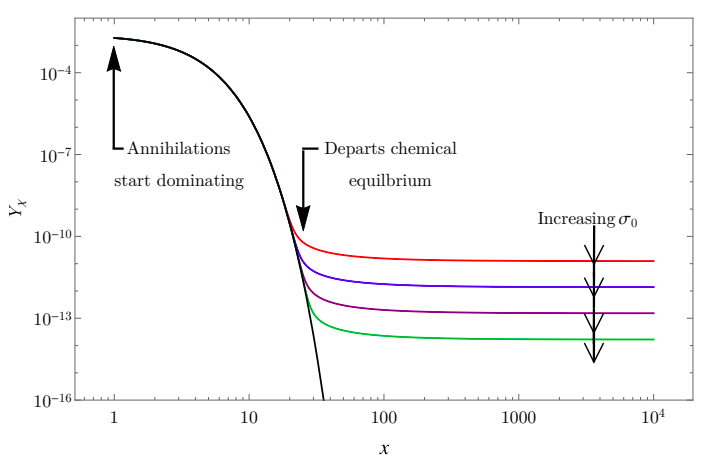
\includegraphics[width=10cm, height=6cm]{figs/FreezeOut.png}
\caption{Schematic representation of the freeze-out process, representing the abundance of a 500 GeV \ac{DM} as $Y_\chi$ with respect to the time and the impact of increasing cross-section annihilation values on this freeze-out abundance \cite{FreezeOut2}.}
\label{figure:FreezeOut}
\end{center}
\end{figure}

All these properties narrow quite a lot the number of possible \ac{DM} candidates, as we will now see in the following section.

\section{Dark matter candidates} \label{section:DMCandidates}

Several different categories of particles could pretend to be good candidates for dark matter but only the most interesting ones will be quoted here, since an extensive list of all the different possible candidates is out of the scope of this work. Two \ac{SM} particles will first of all be investigating, before introducing some \ac{BSM} theories giving us additional \ac{DM} candidates with the expected properties.

\subsubsection*{\acfp{MACHO}}
The first obvious \ac{DM} candidate are the so-called \acp{MACHO}. These objects are massive astronomical non-luminous bodies (such as black holes) made of baryonic matter and very hard to detect, that could be responsible of the gravitational lensing observed and that could explain the apparent missing mass in the Universe. However, as we saw in Section~\ref{section:DMProperties}, \ac{DM} is not expected to be made of such ordinary matter, mainly because observational data of the \ac{CMB} and the deduced baryonic density of energy in the Universe is able to rule out this possibility.

Several different experiments did try to search for such \ac{DM} anyway, and managed to constrain the properties of this kind of objects. The main way to search for such massive objects is through their gravitational lensing effect (actually, we talk about microlensing in this case since this effect is small) since, according to the general relativity principle, they should bend the light of luminous objects located behind them, such as stars, and this bending actually depends on the mass of the eventual \ac{MACHO}. Experiments like the \ac{MACHO} project and EROS observed in this context $\Theta (10^7)$ stars for several years, looking for microlensing events in order to constrain this particular \ac{DM} model. Results published in 2000 from the MACHO project, after studying almost 12 million stars, actually observed between 13 and 17 such events, lower than expected if \ac{DM} was only made of \acp{MACHO}. 

The collaboration actually managed to exclude at the 95\% \ac{CL} the possibility of the dark halo to be entirely made of such baryonic particles \cite{MACHOProject}. On the other hand, the EROS collaboration only observed 1 microlensing after studying more than 30 millions of bright stars during 6.7 years, while $\sim39$ events were expected \cite{EROS}. Both results have also been combined in order to obtain the exclusion plot represented in Figure~\ref{figure:ExclusionMACHO}. From this study, \acp{MACHO} with low masses ($10^{-7}M_\odot < m < 10^{-3}M_\odot$) should make up less than 25\% of the dark matter halo for most models considered at the 95\% \ac{CL} \cite{ExclusionMACHO}.

\begin{figure}[htbp]
\begin{center}
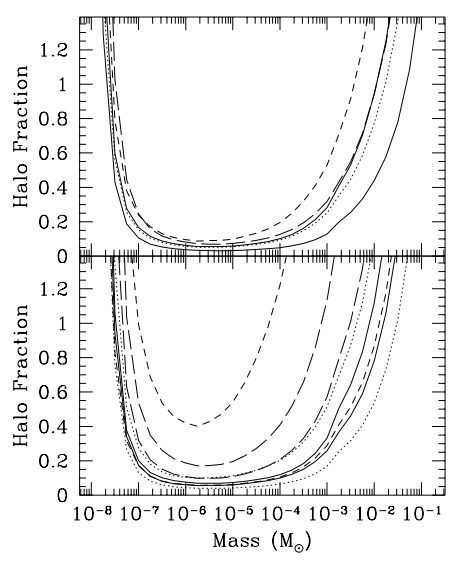
\includegraphics[width=6cm, height=8cm]{figs/MACHOExclusion.png}
\caption{Halo fraction upper limit at the 95\% \ac{CL} compared to the mass of the lensing object for different \ac{MACHO} models considered by the EROS (on the top) and the MACHO (on the bottom) collaborations \cite{ExclusionMACHO}.}
\label{figure:ExclusionMACHO}
\end{center}
\end{figure}

\subsubsection*{Active neutrinos}
\ac{SM} \textit{active} neutrinos $\nu$ (as opposed to \textit{sterile} neutrinos, that will be the subject of the discussion in the next section) have been considered as good \ac{DM} candidates for a long time as well, since they are electrically neutral and long-lived \ac{SM} particles, two important properties of any \ac{DM} candidate. They have a few particular properties that might be interesting in this context.

\begin{itemize}
\item First of all, even though it has still not been measured precisely, the sum of their mass has recently been measured to be lower than 0.17 eV at the 95\% \ac{CL} from cosmological studies \cite{NeutrinoMass}. Even though this is not quite understood, this is incredibly low compared to other \ac{SM} particles, this particularity usually being referred to as the \textit{mass puzzle} of the neutrinos. 

\item Their low mass has a consequence in the sense that it means that the gravitational interaction between two neutrinos is usually considered to be negligible and that we can consider that they only interact weakly, making it hard to study their properties. Their actually cross-section of interaction, as represented in Figure~\ref{fig:NeutrinoXS} and which of course depends on their energies and on the channel of interaction (neutral or charged current considered), is therefore usually extremely low, making it hard to detect neutrinos.

\begin{figure}[htbp]
\begin{center}
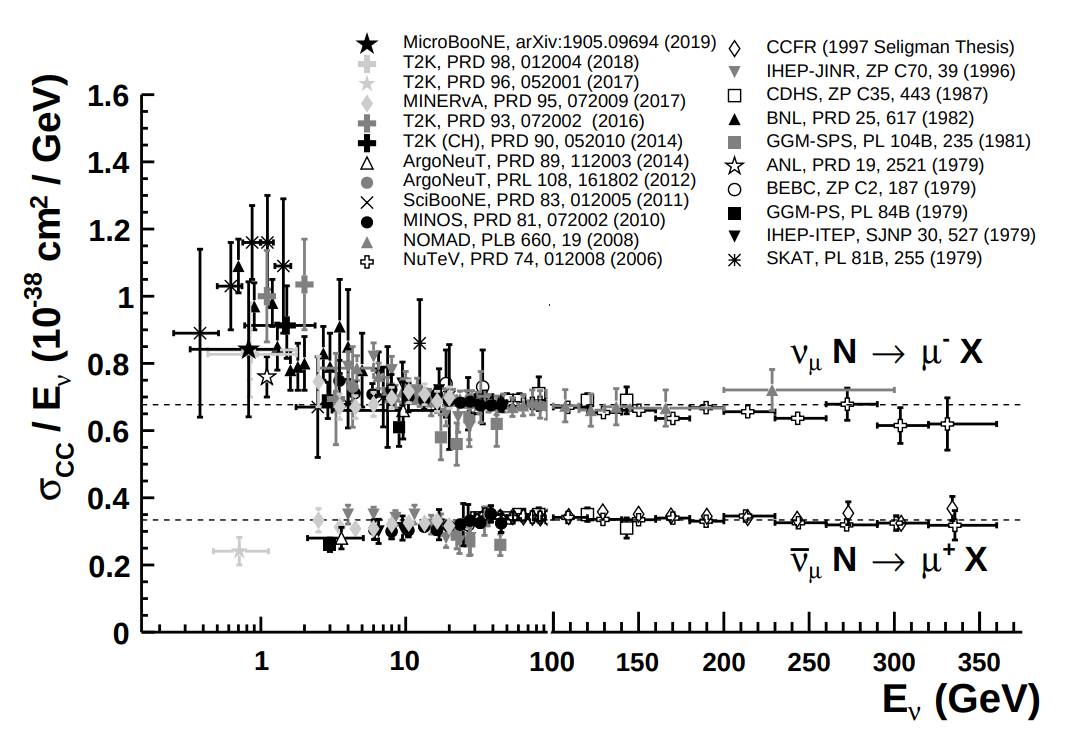
\includegraphics[width=12cm, height=8cm]{figs/NeutrinoXS.png}
\caption{Neutrino cross section of interaction from the charged current as measured by different experiments over a large range of energies, for both neutrinos $\nu$ and antineutrinos $\bar \nu$ \cite{PDGNeutrino}.}
\label{fig:NeutrinoXS}
\end{center}
\end{figure}

This figure clearly shows that an approximate value of the cross section for such neutrinos is of the order of magnitude of $10^{-38}$ cm$^2$ GeV$^{-1}$, which is typically tens of orders of magnitude lower than the interaction cross section of a photon ($\sigma_\gamma \sim 10^{-25}$ cm$^2$ \cite{GammaXS}). This means that the typical neutrinos of a few MeV produced by nuclear reactors have a mean free path of approximately 10 light years in steel.  

\item Neutrinos are also the only \ac{SM} particle only observed in their left-handed chirality state, while anti-neutrinos can only be observed in their right-hand state. This could mean two things: either right-handed neutrinos do not exist in nature for some reason, or we have just not been able to detect them because their interaction with baryonic matter is too weak. Right-handed neutrinos, also referred to as \textit{sterile} neutrinos, do not fit in the current \ac{SM} but could actually also be a strong \ac{BSM} \ac{DM} candidate, as we will discuss in the next subsection.
\item Finally, neutrinos can oscillate, a quantum phenomena according to which the flavor of a neutrino can spontaneously change with time. This means that the three interacting states $\nu_\alpha$ observed are actually composed of several mass eigenstates $\nu_i$, as related in Equation~\ref{eq:Neutrinos}, where these states can be related using the Pontecorvo-Maki-Nakagawa-Sakata matrix $(V_\nu)_{\alpha i}$.

\begin{equation}
\label{eq:Neutrinos}
\nu_\alpha = (V_\nu)_{\alpha i} \nu_i
\end{equation}

This effect does not however at principle have anything to do with the fact that neutrinos can be considered \ac{DM} candidates, so this subject will not be discussed further in this work.
\end{itemize}

However, two physical reasons can explain why we do not really believe that \ac{DM} could be made of neutrinos any more. First of all, their relative abundance does not match the expected one for \ac{DM} from the freeze-out mechanism explained in Section~\ref{section:DMProperties}. Indeed, their freeze-out abundance can be computed quite easily from Equation~\ref{equation:neutrinoRelic} \cite{WIMPBook}, where the sum of the masses of the three neutrino flavors has been calculated to be lower than 0.17 eV \cite{NeutrinoMass} instead of the 11.5 eV expected to obtain the correct \ac{DM} relic abundance as observed today from the power spectrum of the \ac{CMB}. 

\begin{equation}
\label{equation:neutrinoRelic}
\Omega_\nu h^2 = \sum_{i=1}^3 \frac{m_{\nu_i}}{93 \text{ eV}}
\end{equation}

Additionally, for several reasons explained in Section~\ref{section:DMProperties}, a good \ac{DM} candidate is expect to be cold, i.e. non-relativistic. However, being extremely light, neutrinos are expected to be ultra-relativistic and could therefore not be responsible of the emergence of large scale structures as observed today. We can therefore most probably rule out the possibility of \ac{DM} being made of \ac{SM} neutrinos.

\subsubsection*{Sterile neutrinos}
The most obvious \ac{SM} particles being rules out as \ac{DM} candidates, it is now time to introduce some of the most famous \ac{BSM} theories introducing additional particles that could have the properties searched for. The first one of these theories introduce the so-called sterile neutrinos, usually referring to right-handed \ac{SM} neutrinos, as discussed in the previous subsection. 

If they exist, sterile neutrinos are expected to interact in an even weaker way than \ac{SM} active neutrinos, they could be very long-lived as well and in principle, nothing prevents us from considering that they could have a mass superior to 0.4 keV, giving therefore the correct \ac{DM} relic abundance \cite{keVSterile}. A superior bound of 50 keV on such particles can also be obtained considering limits on the observation of the monochromatic decay $\gamma$ line originating from the one loop radiative decay $N \rightarrow \nu + \gamma$ of such particles.

Several experiments are already searching for such particles at this level of energy. Most of these experiments focus on the analysis of $\gamma$-rays and are actually searching for this particular monochromatic line resulting of the decay of sterile neutrinos. Two independent groups actually announced in 2014 the observation of an unidentified emission line at 3.57 keV (Figure~\ref{fig:DMDetection}) which did not match any known atomic emission line and which is actually consistent with an eventual \ac{DM} signal \cite{DMDetection1, DMDetection2}, since most of the possible instrumental contamination effects have been ruled out over the course of the last few years.

\begin{figure}[htbp]
\begin{center}
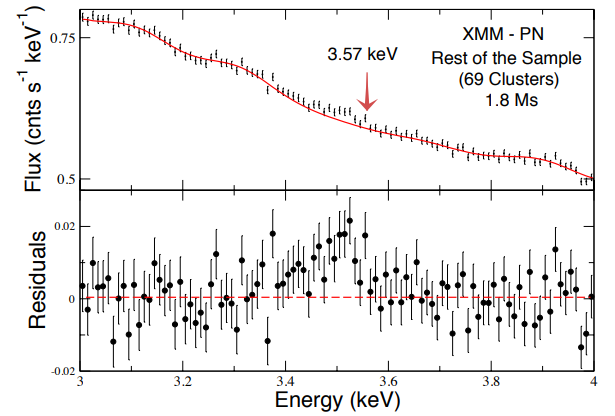
\includegraphics[width=8cm, height=6cm]{figs/DMDetection.png}
\caption{3.57 keV emission line detected with a $4.5 \sigma$ \ac{CL} by the XMM-Newton telescope in 2014, which could be a hint of the presence of \ac{DM} \cite{DMDetection1}.}
\label{fig:DMDetection}
\end{center}
\end{figure}

However, some additional studies of the galactic center pointed out the fact that this observation might actually come from the observation of a potassium K XVIII transition line \cite{NoDetection}. Recent observations actually ruled out at the 99\% \ac{CL} an eventual \ac{DM} origin for this particular line \cite{Nope}, but further studies are still ongoing.

\subsubsection*{Axions}
Axions could also explain the particle nature of \ac{DM}, since their existence could explain 100\% of the \ac{DM} in the Universe, unlike most of the other candidates presented so far. Axions are hypothetical stable neutral particles, with masses of the order of the meV, introduced as a consequence of the strong-CP violation issue of \ac{QCD}. This issue is the following: the usual $\Theta$ term of the \ac{QCD} Lagrangian shown in Equation~\ref{equation:Lag} \cite{QCDLag} should be responsible of breaking the CP symmetry, but this effect has actually never been observed so far: this is the so-called the strong CP problem. 

Two ways to explain that we never observed this phenomena exist: the first is to assume that one of the quarks of the \ac{SM} is massless but this does not match the current observations and measurements. The second consists in assuming that the parameter $\Theta$, the \ac{QCD} vacuum angle, is small enough so that this term becomes negligible. However, by definition, the $\Theta$ angle should be between 0 and $2\pi$, so there is no physical reason for this parameter to be small, unless some new physics can be introduced, as the one developed in 1977 by Peccei and Quinn \cite{Peccei} by relaxing $\Theta$ from a parameter to  a dynamic variable and absorbing it through the introduction of a new pseudoscalar particle that was called the axion.

\begin{equation}
\label{equation:Lag}
\mathcal{L}_\Theta = \frac{\Theta}{32 \pi^2} \epsilon_{\mu \nu \rho \sigma} G_a^{\mu \mu} G_a^{\rho \sigma}
\end{equation}

By definition, it is possible to show that axions satisfy two of the previous criteria for a good \ac{DM} candidate, since they are non-relativistic and their abundance might be enough to account for the dark matter energy density observed, since their actual abundance can easily be computed from Equation~\ref{equation:AxionDensity} \cite{AxionSearches}, from which we could conclude that an axion having a mass of $\sim$20 $\mu$eV could account for the \ac{DM} relic density of the Universe, as observed today. 

\begin{equation}
\label{equation:AxionDensity}
\Omega_a \simeq \left ( \frac{6 \mu \text{eV}}{m_a} \right )^{7/6}
\end{equation}

Several axions searches experiments have therefore been set up, such as the \ac{ADMX}, a resonant microwave cavity installed at the University of Washington, \ac{CAST}, a CERN experiment observing the Sun which came online in 2002 and which managed in 2014 to turned up definitely the existence of solar axions \cite{CASTLimit}, or the \ac{IAXO}, whose aim would be to search for axions with a much better signal to ratio noise than \ac{CAST}. All the results obtained by these experiments along with their future projections are represented in Figure~\ref{figure:AxionSummary}.

\begin{figure}[htbp]
\begin{center}
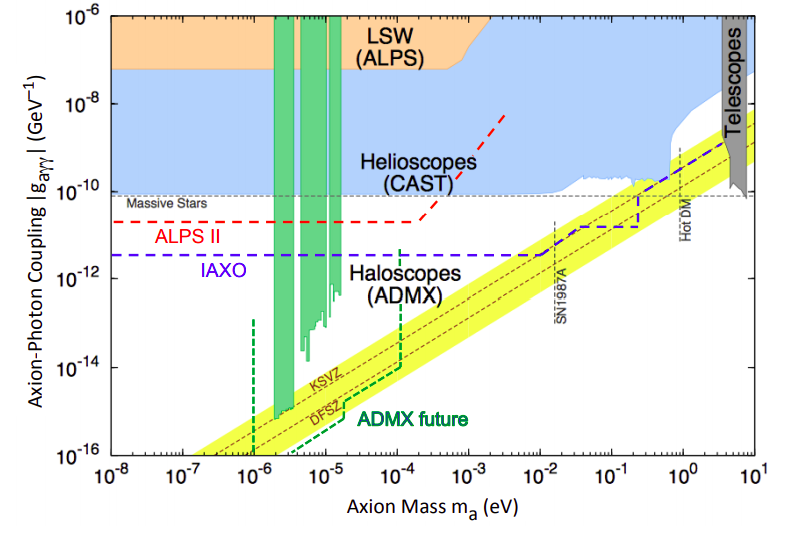
\includegraphics[width=12cm, height=8cm]{figs/AxionSummary.png}
\caption{Axions exclusion plot summary and projected coverage of axion searches experiments, such as \ac{ADMX}, \ac{CAST} and \ac{IAXO} \cite{AxionSearches}.}
\label{figure:AxionSummary}
\end{center}
\end{figure}

\subsubsection*{\acfp{WIMP}} 
The actual \ac{DM} candidate that will be mostly considered throughout this work are the so-called \acfp{WIMP}, which are expected to interact, even though very weakly, with ordinary baryonic matter and which have an expected mass in the range of 100 GeV to 1 TeV for reasonable electroweak production cross-section values, right where we expect \ac{DM} to be found from its relic density: this is the so-called "WIMP miracle", an important concept that can be translated mathematically as well. Indeed, because of the freeze-out scenario explained in Section~\ref{section:DMProperties}, we can find an expression relating the relic abundance of \ac{DM} $\Omega_\chi$ with its annihilation cross section $\langle \sigma_A v \rangle$ through Equation~\ref{eq:Annihilation} \cite{IndirectSearches}.

\begin{equation}
\label{eq:Annihilation}
\Omega_\chi h^2 \sim \frac{3 \cdot 10^{-27} \text{ cm}^3 \text{ s}^{-1}}{\langle \sigma_A v \rangle}
\end{equation}

This equation implies that, since we do know the current abundance of \ac{DM} in the Universe, the total annihilation cross section of \ac{DM} should be equal to $\sim 3 \cdot 10^{-26} $ cm$^3 $ s$^{-1}$, which corresponds to the typical value given by \acp{WIMP} for a range of dark matter masses matching the expected one.

Several strategies can be used to detect such particles, as we will now see in the Section~\ref{section:DMSearches}. This kind of particle basically arises in various \ac{BSM} theories, such as the lightest supersymmetric particle in SUSY. According to this theory, each \ac{SM} particle should have a superpartner whose quantum numbers would be identical except for their spins, which would differ by one half. All of these superpartners would then be potentially new and undiscovered particles, giving us a perfect \ac{DM} candidate in most of the \ac{MSSM} theories, the neutralino $\chi$.

The \acp{WIMP} are also interesting in the sense that introducing them in the terms of this supersymmetric theory would not only give us a strong \ac{DM} candidate, but would also solve the hierarchy problem, the apparent large discrepancy between multiple aspects of the weak and gravitational forces ($10^{24}$ less times stronger).

\section{Dark matter searches} \label{section:DMSearches}

As previously stated, several cosmological evidences allow us to introduce the concept of dark matter, but its properties such as its mass, coupling and interaction cross-section are difficult to study in this context. Several different ways can then be used in order to try and detect \ac{DM} particles in order to study them, as represented in Figure~\ref{fig:ThreeWays}, strategies which can usually be divided into three categories: the direct and indirect searches, mostly relying on the production of baryonic matter from the interaction between two \ac{DM} particles or on the observation on the interaction between the dark and baryonic sectors, and the production in colliders, usually able to probe lower \ac{DM} candidates masses and which will actually be the main focus of this work. 

A discussion about these different detection strategies along with the main results obtained by different experiments in each case will now be presented.

\begin{figure}[htbp]
\begin{center}
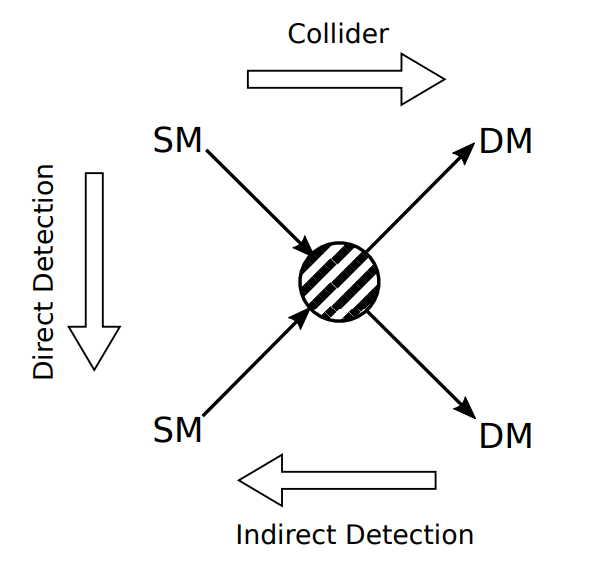
\includegraphics[width=5.5cm, height=5cm]{figs/ThreeWays.png}
\caption{Schematic view of the three main \ac{DM} detection strategies: direct, indirect and collider production searches \cite{ColliderSearches}.}
\label{fig:ThreeWays}
\end{center}
\end{figure}

\subsection{Direct searches} \label{subsection:DirectSearches}

From cosmological observations, we know that we live in a halo of dark matter. In this case, \ac{WIMP}s should cross the Earth every day and, even if they interact only weakly, we should be able to directly detect them through their interaction with ordinary baryonic matter, for example because of their scattering with the nuclei of these particles. Indeed, the transfer of momentum between these two particles in this case might be detectable with the correct experimental device, typically placed deep underground to have the lowest possible background, which is the main source of perturbations of such experiments. 

To study this particular category of searches, let's first of all introduce the rate of expected WIMP scattering off a target nucleus of mass $m_N$ with Equation~\ref{equation:WIMPRate}, rate which ends up being described by a simple steeply
falling exponential function as shown in Figure~\ref{fig:DirectFalling} \cite{DirectSearches}, where $E_{nr}$ is the nuclear recoil energy measured, $m_\chi$ is the \ac{WIMP} mass, $\sigma$ its cross section, $\rho_0 = 0.3$ GeV cm$^{-3}$ is the local dark matter density and $f(v)$ the normalized \ac{WIMP} velocity distribution.

\begin{equation}
\label{equation:WIMPRate}
\frac{dR}{dE_{nr}} = \frac{\rho_0 M}{m_N m_\chi} \int_{v_{\text{min}}}^{v_{\text{esc}}} v f(v) \frac{d \sigma}{dE_{nr}}dv \propto exp \left (- \frac{E_{nr}}{E_0} \frac{4 m_\chi m_N}{(m_\chi + m_N)^2} \right )
\end{equation}

\begin{figure}[htbp]
\begin{center}
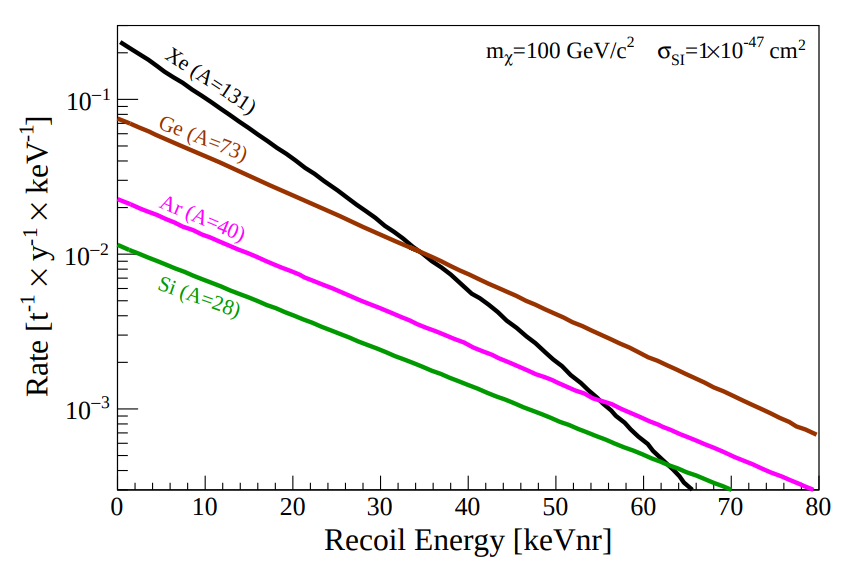
\includegraphics[width=10cm, height=7cm]{figs/DirectFalling.png}
\caption{ Nuclear recoil spectra induced in different materials for a given \ac{DM} \ac{WIMP} of 100 GeV, assuming a WIMP-nucleon \ac{SI} cross section \cite{DirectSearches}.}
\label{fig:DirectFalling}
\end{center}
\end{figure}

From this relation, the Equation~\ref{eq:Number} can be easily derived, representing this time the number of expected \ac{DM} events in an experiment running during a time $T$, where $\epsilon(E_{nr})$ is the efficiency of the detector for a given recoil energy.

\begin{equation}
\label{eq:Number}
N = T \int_{E_{\text{min}}}^{E_{\text{max}}} \epsilon(E_{nr}) \frac{dR}{dE_{nr}} \text{ } dE_{nr}
\end{equation}

The maximal velocity $V_{\text{esc}}$ used as superior bound of the integral in Equation~\ref{equation:WIMPRate} has actually been measured to be in the range $[498-608]$ km/s at the 90\% \ac{CL} \cite{EscapeVelocity}, since any particle having a velocity higher than this would not be bound any more to the gravitational potential of a galaxy. This has an important consequence: all the direct and indirect detection experiments actually need to take into account is the annual modulation of the observed count rate, due to the movement of the Earth around the Sun, as shown in Figure~\ref{fig:AnnualModulation} \cite{AnnualModulation}, since this velocity is not negligible compared to the escape velocity $v_{\text{esc}}$. 

\begin{figure}[htbp]
\begin{center}
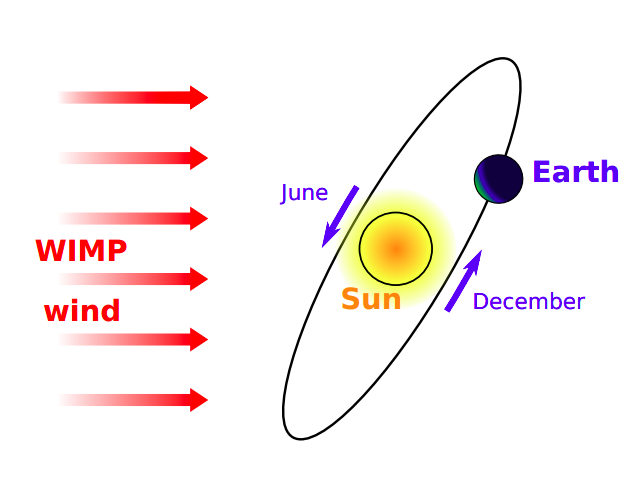
\includegraphics[width=8cm, height=6cm]{figs/AnnualModulation.png}
\caption{Schematic representation of the annual modulation of the WIMP wind introduced by the motion of rotation of the Earth around the Sun \cite{AnnualModulation}.}
\label{fig:AnnualModulation}
\end{center}
\end{figure}

From our perspective, it seems indeed that the velocity of the speed of \ac{WIMP} particles arriving is changing depending on the month of the year, since the Earth is sometimes moving in the direction of the \ac{WIMP} source, and is sometimes moving away: the maximal velocity is reached around June. This is extremely important to take into account this effect since, as we saw on the previous equations such as Equation~\ref{eq:Annihilation}, the count rate of incoming particles $N(t)$ actually depends on this velocity, and this modulation then introduces a periodical modulation that we need to take into account, as shown in Equation~\ref{eq:Modulation}, where the periodical part usually introduces a $\sim5$\% deviation \cite{DirectSearches}.

\begin{equation}
\label{eq:Modulation}
N(t) = B + N_0 + N_m cos(\omega (t-t_0))
\end{equation}

This effect is also important because an experiment performed during a long period of time can actually help us finding an eventual hint of \ac{DM} particles, since our signal is expect to follow this periodical deviation while the background is expected to be constant. Moreover, this \ac{WIMP} wind is expected to come from a particular region of the sky while the backgrounds are expected to be distributed uniformly, so this gives a clear way to isolate the signal.

Finally, it is also important to note that two different kinds of direct searches can be defined, depending on the category of the scattering between the \ac{DM} and the nucleus: the \acf{SI} (proceeding through the scalar term) and \acf{SD} (proceeding through the axial term of the Lagrangian) searches, since the interaction cross section $\sigma$ of Equation~\ref{equation:WIMPRate} is expected to be different for \ac{DM} particles having a spin 0 or not, as shown in Equation~\ref{eq:SISD}, where $F$ is a factor accounting for the dependence of the scattering on the energy. This means that results obtained by either hypothesis can usually not be compared with each other.

\begin{equation}
\label{eq:SISD}
\frac{d\sigma}{dE_{nr}} \propto \sigma_{SI} F_{SI}^2(E_{nr}) + \sigma_{SD} F_{SD}^2(E_{nr})
\end{equation}

As previously stated, many experiments are dedicated to the direct search of \ac{DM} particles, but in order to isolate an eventual \ac{DM} signal, an environment with an ultra-low background is usually required, which can usually be reduced either by placing the detector underground (to reduce the contamination due to the cosmic rays), by increasing the statistics or by choosing carefully the active material of the detector (to reduce the internal background coming from the detector itself). The impact these kind of parameters have on the final limits can be seen in Figure~\ref{fig:ImpactLimit}.

\begin{figure}[htbp]
\begin{center}
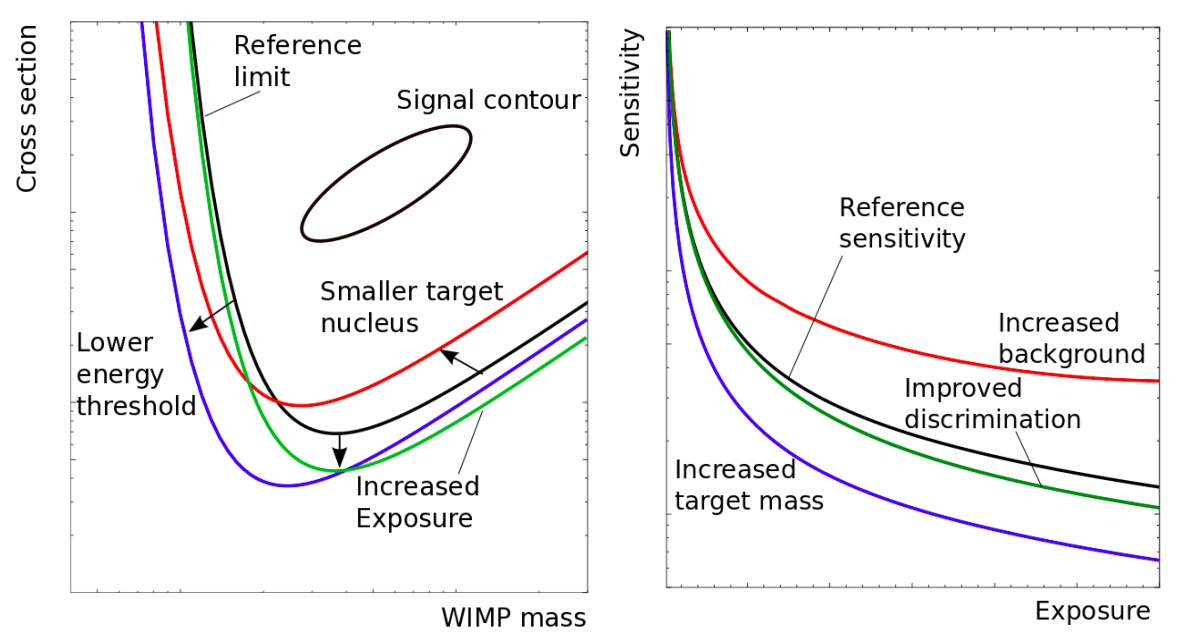
\includegraphics[width=14cm, height=7cm]{figs/ImpactLimits.png}
\caption{Impact of different experimental parameters on the final limits depending on the cross section and \ac{WIMP} mass (on the left) or sensitivity and exposure (on the right), with respect to the expected limits (black curve) \cite{DirectWays}.}
\label{fig:ImpactLimit}
\end{center}
\end{figure}

These detectors try to detect the scattering of an unknown exotic particle with an ordinary nucleus, which typically can give rise to different categories of signals. Some detectors try for example to detect the direct ionization of the target atom, while others focus on the emission of light coming from the desexcitation of the scattered nucleus, and some even search for the heat produced by these collisions under the form of phonons in a crystal. All these different search strategies have been summarized schematically in Figure~\ref{figure:DirectWays}.

\begin{figure}[htbp]
\begin{center}
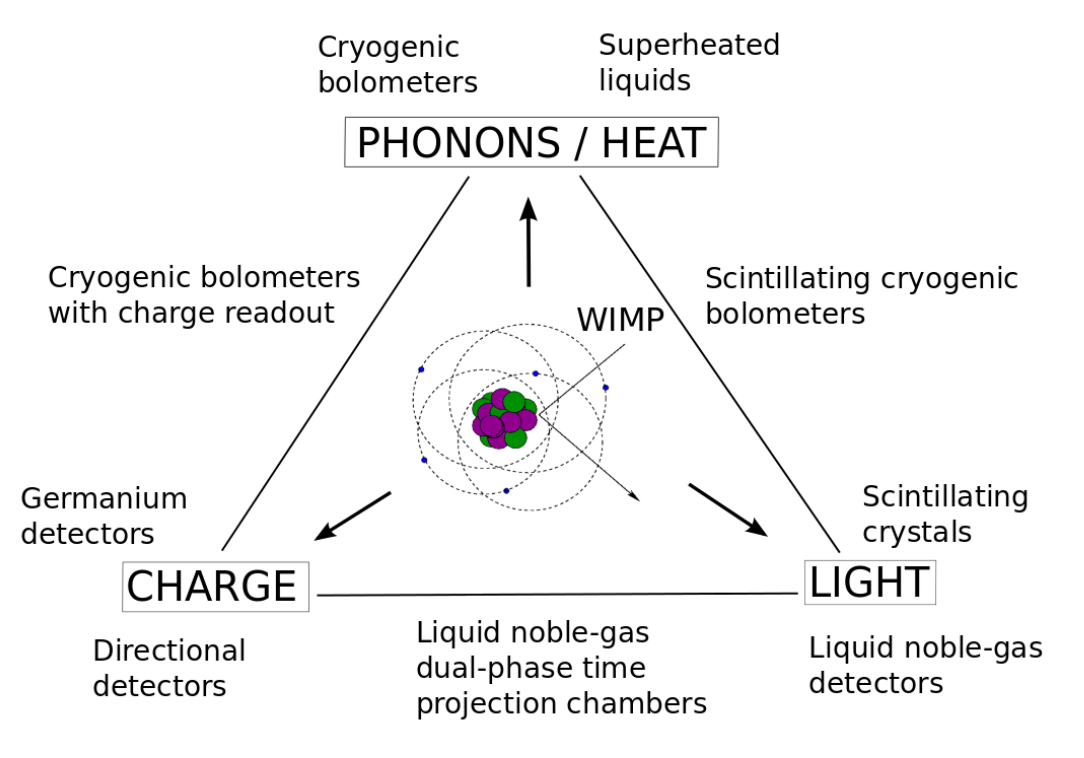
\includegraphics[width=12cm, height=8cm]{figs/DirectWays.png}
\caption{Schematic representation of the three main strategies to detect directly the interaction between \ac{DM} particles and an ordinary nucleus \cite{DirectWays}.}
\label{figure:DirectWays}
\end{center}
\end{figure}

As of today, no direct experiment has been able to detect serious hints for the existence of \ac{DM}, and they have only been able to set limit on the scattering cross section depending on the models parameters, as seen on Figure~\ref{fig:DirectLimits} for multiple experiments at once.

\begin{figure}[htbp]
\begin{center}
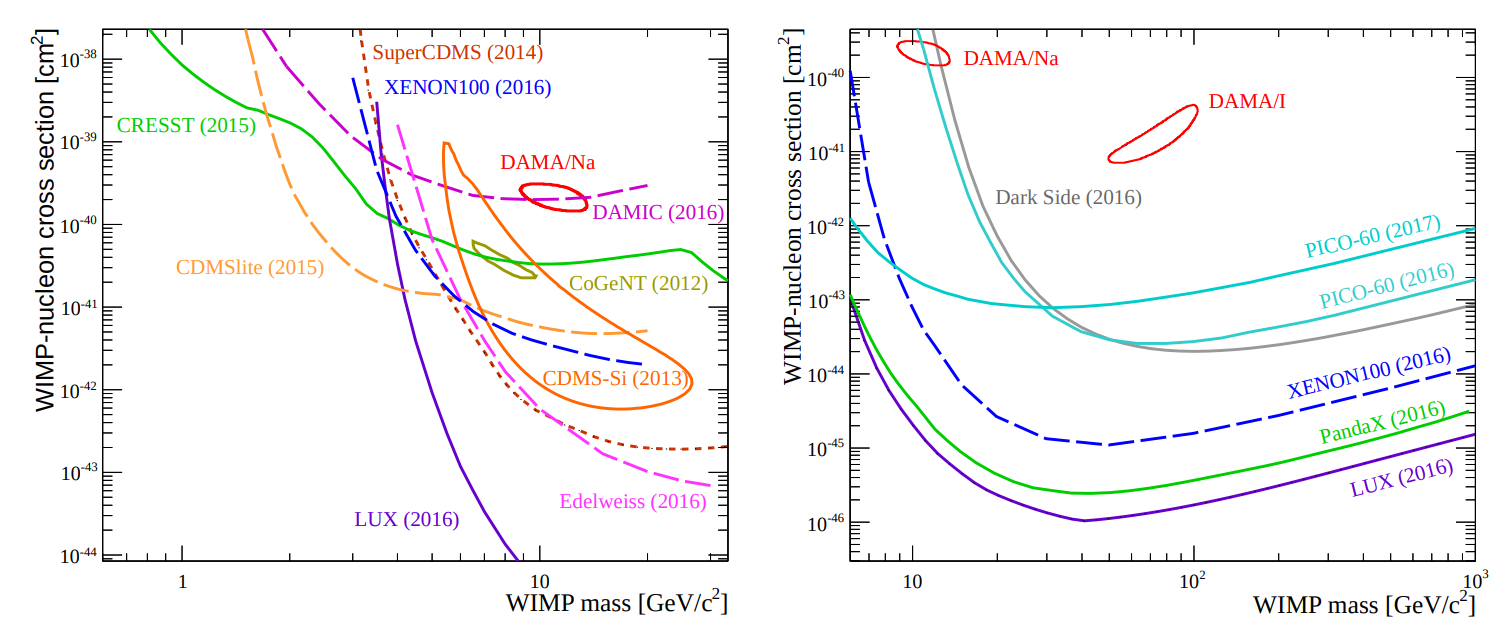
\includegraphics[width=14cm, height=6cm]{figs/DirectLimits.png}
\caption{Exclusion limits obtained by various direct detection experiments considering a \ac{SI} interaction cross section for low \ac{WIMP} (on the left) or high \ac{WIMP} masses (on the right) \cite{DirectWays}.}
\label{fig:DirectLimits}
\end{center}
\end{figure}

However, the DAMA experiment at the \ac{LNGS} did find an interesting result by showing the hints of an annual modulation signal compatible to the expected one due to the \ac{WIMP} wind in the 2-6 keV energy range, as seen on Figure~\ref{fig:DAMA} \cite{DAMA}. Further investigations about this modulation are still ongoing today, since no systematic effect able to account for the observed modulation amplitude and to simultaneously satisfy all the requirements of the signature has been found so far.

\begin{figure}[htbp]
\begin{center}
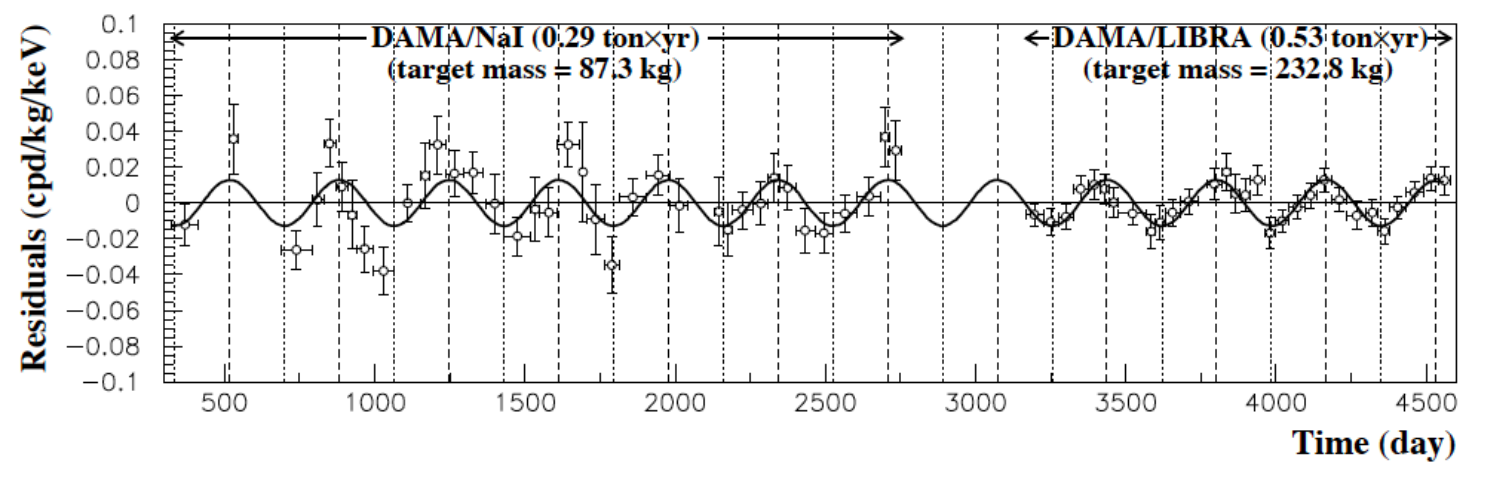
\includegraphics[width=14cm, height=5cm]{figs/DAMA.png}
\caption{Observed and expected annual modulation in single hits events in the 2-6 keV energy range by the DAMA experiment \cite{DAMA}.}
\label{fig:DAMA}
\end{center}
\end{figure}

\subsection{Indirect searches}

The indirect detection of \ac{DM} particles consists basically in searching for \ac{SM} products coming from the annihilation of two \ac{DM} particles or from its eventual direct decay, usually under the form of a flux of $\gamma$-rays, neutrinos, cosmic-rays or anti-matter appearing as an excess over the expected background. Indeed, many extensions to the \ac{SM}, such as the supersymmetry SUSY or \ac{UED} do provide solid \ac{DM} candidates (the lightest supersymmetric particle and the lightest Kaluza-Klein state, respectively) expected to interact with each other, resulting in the immediate production of \ac{SM} (un)stable particles that can be detected by telescopes either placed on the ground or directly in space. Another point to make is that indirect searches are also usually affected by the annual fluctuation induced by the movement of the Earth around the Sun, as explained in the previous Section~\ref{subsection:DirectSearches}.

Indirect searches are actually extremely useful since they are sensitive to the \ac{DM} annihilation cross section, mass and the density profile of \ac{DM} halos $\rho(\overrightarrow{r}(s, \Omega))$, usually represented by a \ac{NFW} profile, as shown in Equation~\ref{eq:NFW} \cite{FluxIndirect}, where $r_s = 20$ kpc is the scale radius of the \ac{DM} halo for the Milky Way and $r$ is the distance to the center of the cluster considered, assumed to be spherical in this case.

\begin{equation}
\label{eq:NFW}
\rho(r) \propto \frac{r_s}{r \cdot \left (1+\frac{r}{r_s})^2 \right )}
\end{equation} 

The flux coming from the annihilation of two \ac{DM} particles is then expected to be proportional to its annihilation cross section $\sigma v$, the solid angle of observation $\Omega$ and the number of particles emitted by this annihilation $\frac{dN}{dE}$, according to Equation~\ref{eq:FluxIndirect}, where the integration is done over the line of sight $l$ and the solid angle of observation $\Omega$.

\begin{equation}
\label{eq:FluxIndirect}
\frac{d \Phi}{d\Omega dE} = \frac{\sigma v}{8 \pi m_\chi^2} \cdot \frac{dN}{dE} \iint_{l, \Omega} \rho^2(\overrightarrow{r}(s, \Omega)) \text{ } dl \text{ } d\Omega \equiv P \cdot J(\Delta \Omega)
\end{equation} 

This equation is extremely important for two reasons. First of all, it shows that, if a signal is found in direct detection, we could use this detection to determine the new object mass and scattering cross section and then use this information in order to obtain the \ac{DM} density profile this way: the data obtained by the different strategies of detection are actually complementary. The second reason is that as we can see, the flux of incoming particles can actually be divided into two factors: $P$, entirely dependent on the physics of the \ac{DM} particle, and the J-factor $J(\Delta \Omega)$, depending only on the distribution of \ac{DM} within the system considered. This J-factor is in this sense actually a measurement of the quality of an astronomical object for an indirect measurement, since the higher the flux received, the better the measurement will be in general (even though this is not the only factor which matters, since for example the galactic center has a higher J-factor than the best dwarf galaxy observable, but also has a lot of backgrounds affecting the measurement).

As different channels of observations are available for us to analyze the eventual annihilation of \ac{DM}, several strategies can be used in order to detect \ac{DM} indirectly, as we will now see, by searching different kind of \ac{SM} particles. Anyway, all these strategies have one goal in common: try to reduce the background, since the signal searched for is usually quite low while the uncertainties associated to the background in astrophysics are usually quite high.

\subsubsection*{Through $\gamma$-rays detection}
The golden channel for such searches are through the production of $\gamma$-rays by \ac{DM} annihilation $\chi \chi \rightarrow \gamma + X$ or decay $\chi \rightarrow \gamma + X$, mainly because the energy scale of the \acp{WIMP} implies that most of the annihilation and decay radiation will be emitted in this range of energies and because $\gamma$-rays are usually not deflected when traveling to the observer (this means that the exact source of this kind of radiation can be quite easily and precisely pin-pointed). However, they do have one drawback as well: the Earth's atmosphere is usually opaque to this kind of radiation at this level of energy. This means that most of experiments searching for them simply cannot be performed from the ground and have to be sent to space. 

One of the most famous detectors of this category is the \ac{LAT}, a pair production detector launched in June 2008 and mostly sensitive to $\gamma$-rays between 20 MeV and 300 GeV \cite{LATExperiment}. This experiment has managed to exclude a large portion of the phase space, as seen in Figure~\ref{figure:LATExclusion}. The GAMMA-400 experiment, whose launch is scheduled in 2020, will pick up the work of \ac{LAT}, by studying a similar range but with a much improved angular and energy resolutions \cite{GAMMA400}. 

\begin{figure}[htbp]
\begin{center}
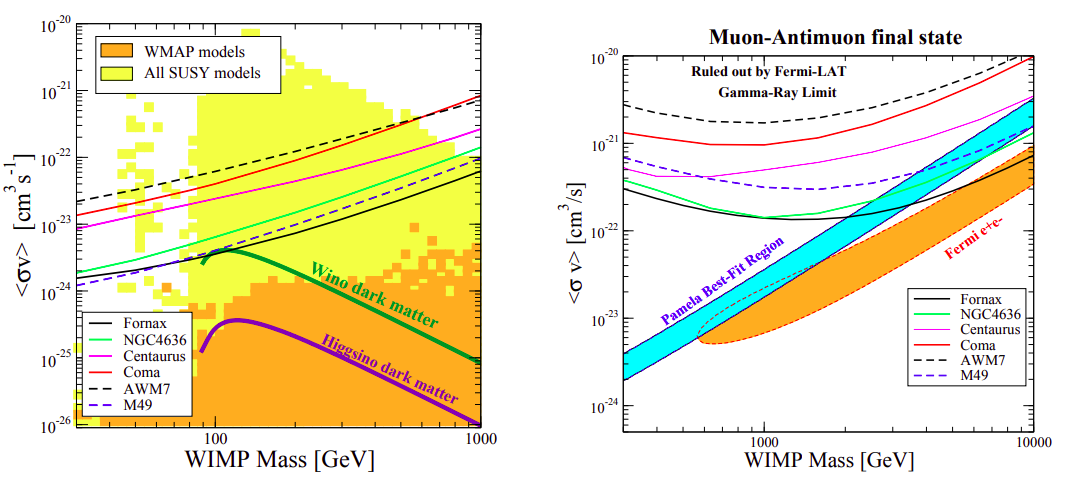
\includegraphics[width=12cm, height=6cm]{figs/LATExclusion.png}
\caption{Upper limits on the \ac{DM} annihilation cross section considering $b \bar b$ (on the left) and $\mu^+ \mu^-$ (on the right) final states as a function of the \ac{WIMP} mass, for different clusters studied \cite{LATExperiment}.}
\label{figure:LATExclusion}
\end{center}
\end{figure}

It is much harder for \ac{DM} to produce high energy $\gamma$-rays and therefore, the flux of such particles decreases quite quickly with energy, making it harder to study since telescopes then need a much larger effective area to pick up the same quantity of signal, and have therefore to be put on the ground. Such telescopes do exist, are called \ac{IACT} and have to take into account the atmospheric perturbations to work in an optimal way. They are usually sensitive to a range of energies going from $\sim 10$ GeV up to $\sim 100$ TeV, but can usually only study a small portion of the sky (up to a few degrees), forcing these experiments to choose carefully the objects to be studied. The \ac{CTA} is a brand new telescope of this kind whose construction is supposed to start this year, that should improve greatly the sensitivity of high masses indirect \ac{DM} searches.

\subsubsection*{Through neutrinos detection}
Interacting only weakly, neutrinos are another reliable source of data in the Universe since they are not supposed to be altered when traveling large distances as well, even though detecting neutrinos is usually much harder than detecting $\gamma$-rays and usually involves huge thanks of water in which neutrinos can produce a Cherenkov effect that will eventually be detected.

The most famous detector of this kind, the IceCube neutrino observatory, actually uses the ice of the South Pole instead of water to detect these particles with photo-detectors, mainly because of the low interaction cross section of the neutrinos which then require the installation of a huge volume of material to increase the probability of interaction. Super-Kamiokande (Super-K), in Japan, is another large Cherenkov experiment dedicated to the detection of cosmic neutrinos. Both detectors are also largely involved as direct searches experiments, since they are also sensitive to the eventual recoil between \ac{DM} and ordinary matter nuclei.

The problem with this kind of experiment is the difficulty of actually detecting some neutrinos, along with the background levels from atmospheric neutrinos, as represented in Figure~\ref{fig:BkgNeutrino}, typically several orders of magnitude larger than the signal. Several strategies therefore need to be put in place in order to reduce the background level in such experiments, such as the study of the directionnality of the source and an appropriate choice of angle of observation, since most of the contamination is coming from tau neutrinos, themselves originating from muon neutrinos oscillation, strongly suppressed around the zenith.

\begin{figure}[htbp]
\begin{center}
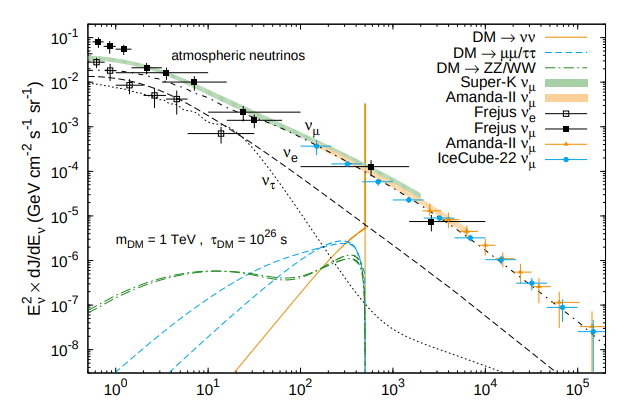
\includegraphics[width=12cm, height=8cm]{figs/BkgNeutrino.png}
\caption{Neutrino spectra for a scalar \ac{DM} candidate of 1 TeV for different indirect detection experiments and the corresponding background level expected \cite{BkgNeutrino}.}
\label{fig:BkgNeutrino}
\end{center}
\end{figure}

\subsubsection*{Through cosmic rays detection}

Searching for anti-matter in the cosmic rays presents the advantage of being highly sensitive, because of the low levels of backgrounds this kind of searches implies. However, cosmic rays are affected when traveling through the Universe, and determining the exact location of their emission can be quite challenging.

Among the most famous detectors of this kind, we can quote PAMELA, a spatial telescope dedicated to the study of such cosmic rays since 2006. \ac{CERN}'s \ac{AMS}, installed in the International Space Station has also studied such radiation from a range of a few hundred MeV up to 1 TeV. The data collected by this detector is compared to the exclusion limits obtained by the IceCube detector in Figure~\ref{fig:AMSData}.

\begin{figure}[htbp]
\begin{center}
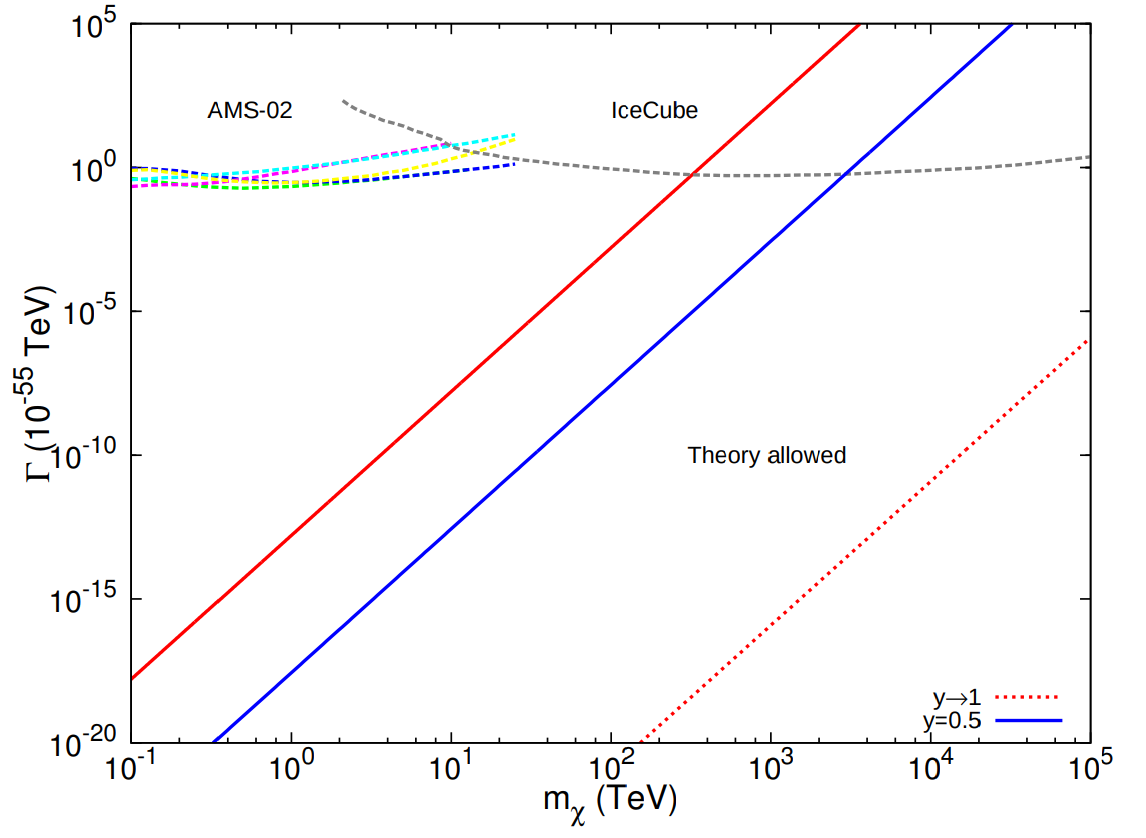
\includegraphics[width=10cm, height=7cm]{figs/AMSData.png}
\caption{Limits of the decay width of the interaction with respect to the \ac{DM} mass obtained by both IceCube and \ac{AMS} \cite{AMSData}.}
\label{fig:AMSData}
\end{center}
\end{figure}

%In summary, indirect searches are extremely important searches towards an eventual detection of \ac{DM} particles. In this case, the annihilation and the decay of the \ac{DM} can be studied, while several decay modes are possible and several strategies can be employed. The most effective search strategy is through the study of $\gamma$-rays, even though this has the 

\subsection{Collider production} \label{subsection:ColliderProduction}

In this particular kind of searches, we are particularly interested in the eventual direct production of \ac{DM} candidates following the collision between two highly energetic \ac{SM} particles, a perfectly viable scenario if we keep assuming that \ac{DM} should at least interact weakly with ordinary matter if we want to be able to produce or detect it in a laboratory.

In this case, two main models for the interaction between \ac{SM} and \ac{DM} particles can be considered, each with a different level of complexity and different possible applications:

\begin{itemize}
\item The \ac{EFT} approach is usually considered to be the easiest and most simplified one, even though it can still give us plenty of information about this kind of interaction. It relies on a strong assumption, assuming that the energy scale of the new exotic physics is much larger than the actual energy accessible with our experiment, since the momentum transfer of this interaction needs to be much smaller than the mediator mass for this simplified approach to be valid.

According to this approach, represented in Figure~\ref{fig:EFT}, the interaction can be described using simplified operators (the most simple ones being either scalar $\bar \chi \chi \bar q q$, pseudoscalar $\bar \chi \gamma^5 \chi \bar q \gamma^5 q$, vector $\bar \chi \gamma^{\mu} \chi \bar q \gamma_\mu q$ or axial-vector $\bar \chi \gamma^\mu \gamma^5 \chi \bar q \gamma_\mu \gamma^5 q$) since, according to the assumption made, its mediator can usually be integrated out \cite{ColliderSearches}. 

Despite of this strong assumption, this approach is actually quite useful anyway in the sense that it is able to provide us bounds on the new physics scale $\Lambda$, which can be related to the different couplings of the interaction as in Equation~\ref{eq:EnergyScale}, where $g_q$ and $g_\chi$ are the coupling between the mediator and the \ac{SM} or \ac{DM} particle, and $m_{\text{med}}$ is the mass of the mediator. 

\begin{equation}
\label{eq:EnergyScale}
\frac{1}{\Lambda^2} = \frac{g_q g_\chi}{m_{\text{med}}}
\end{equation}

Additionally, direct searches experiments typically also introduce this kind of assumptions to extract constraints from their measurements, making it straightforward to compare the results obtained in both approaches. However, the transfer of momentum in the direct searches experiments is usually of the order of a few keV as seen in Equation~\ref{eq:MomentumTransfer}, while in collider experiments such as the \ac{LHC}, this is of the order of $\Theta$(GeV-TeV).

\begin{equation}
\label{eq:MomentumTransfer}
E = \frac{m_\chi v_\chi^2}{2} \simeq 100 \text{ GeV} \cdot 10^{-6} \simeq 50 \text{ keV}
\end{equation}

This means that, especially due to the increasing center of mass energy given by the \ac{LHC} over the last few years, the basic \ac{EFT} assumption is usually not respected and gives information about an out of reach phase space region anyway, making its usefulness quite relative in most cases. This is why more complex models need to be developed as well.

\item The simplified models attempt to solve the issue related to the approximation made by the \ac{EFT} approach, by increasing the level of details regarding the interaction between the dark and baryonic sectors. This is usually done by explicitly taking into account the mediator of the interaction, which can be considered of two different types in the context of this work: either scalar $\phi$ or pseudoscalar $a$ (both having a spin 0), described by the Lagrangians in Equation~\ref{eq:MedLag}, considering the \ac{DM} candidate to be a Dirac fermion coupling to the \ac{SM} through the mediator considered and under the assumption of \acf{MFV}. In this equation, the sum runs over the three \ac{SM} families and the parameters $y_i^f = \sqrt{2} \frac{m_i^f}{v}$ are the Yukawa couplings, much larger for the top quarks because of their mass, which will allow us to simplify the following equations \cite{SimplifiedModels}.

\begin{equation}
\label{eq:MedLag}
\begin{dcases}
\mathcal{L}_{\text{fermion}, \phi} \propto - g_\chi \phi \bar \chi \chi - \frac{\phi}{\sqrt{2}} \sum_i \left (g_u y_i^u \bar u_i u_i + g_d y_i^d \bar d_i d_i + g_l y_i^l \bar l_i l_i \right ) \\
\mathcal{L}_{\text{fermion}, a} \propto - i g_\chi a \bar \chi \gamma^5 \chi - \frac{i a}{\sqrt{2}} \sum_i \left (g_u y_i^u \bar u_i \gamma^5 u_i + g_d y_i^d \bar d_i \gamma^5 d_i + g_l y_i^l \bar l_i \gamma^5 l_i \right )
\end{dcases}
\end{equation}

An important parameter in this case is the decay width of this mediator $\Gamma_{\text{med}}$, given by Equation~\ref{eq:WidthMed} for either a scalar mediator $\phi$ or Equation~\ref{eq:WidthMedPseudo} for a pseudoscalar mediator $a$, where the first term corresponds to the mediator decay to \ac{SM} particles, the second to its decay to \ac{DM} particles and the last term its possible decay to gluons. 

\begin{equation}
\label{eq:WidthMed}
\begin{dcases}
\Gamma_{\phi} = \sum_f N_C \frac{y_f^2 g_\nu^2 m_\phi}{16 \pi} \left (1- \frac{4 m_f^2}{m_\phi^2} \right )^{3/2} + \frac{g_\chi^2 m_\phi}{8 \pi} \left (1- \frac{4 m_f^2}{m_\phi^2} \right )^{3/2} + \frac{\alpha_S^2 g_\nu^2 m_\phi^3}{32 \pi^3 \nu^2} \left \lvert f_\phi \left (\frac{4m_t^2}{m_\phi^2} \right ) \right \rvert^2 \\
f_\phi(\tau) = \tau \left (1 + (1 - \tau) \text{ arctan}^2 \left ( \frac{1}{\sqrt{\tau -1}} \right ) \right )
\end{dcases}
\end{equation}

\begin{equation}
\label{eq:WidthMedPseudo}
\begin{dcases}
\Gamma_{a} = \sum_f N_C \frac{y_f^2 g_\nu^2 m_a}{16 \pi} \left (1- \frac{4 m_f^2}{m_a^2} \right )^{1/2} + \frac{g_\chi^2 m_a}{8 \pi} \left (1- \frac{4 m_f^2}{m_a^2} \right )^{1/2} + \frac{\alpha_S^2 g_\nu^2 m_a^3}{32 \pi^3 \nu^2} \left \lvert f_a \left (\frac{4m_t^2}{m_a^2} \right ) \right \rvert^2 \\
f_a(\tau)= \tau \text{ arctan}^2 \left (\frac{1}{\sqrt{\tau -1}} \right )
\end{dcases}
\end{equation}

In the case of the simplified models, the minimal set of parameters describing the interaction is therefore $\{m_\chi, \text{ } m_{\text{med}}, \text{ } g_\chi, \text{ } g_q \}$.

\begin{figure}[htbp]
\begin{center}
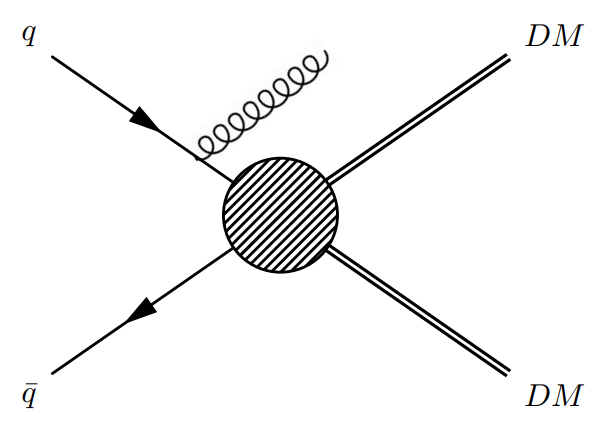
\includegraphics[width=5.5cm, height=4cm]{figs/EFT.png}
\caption{Schematic representation of a typical \ac{EFT} modelization of an \ac{LHC} event with an \ac{ISR} object used to trigger the event \cite{ColliderSearches}.}
\label{fig:EFT}
\end{center}
\end{figure}

\end{itemize}

An additional categorization of the \ac{DM} production models can be done, by separating the so-called s-channel and t-channel models, as shown in Figure~\ref{fig:STChannels}. In the first case, the most common one in collider searches, the mediator between the \ac{SM} and \ac{DM} is assumed to be a boson, and usually decays directly into a pair of \ac{DM} particles. On the other hand, in the t-channel models, the mediator couples to one quark and one \ac{DM} particle, with a colored exchange particle required.

\begin{figure}[htbp]
\begin{center}
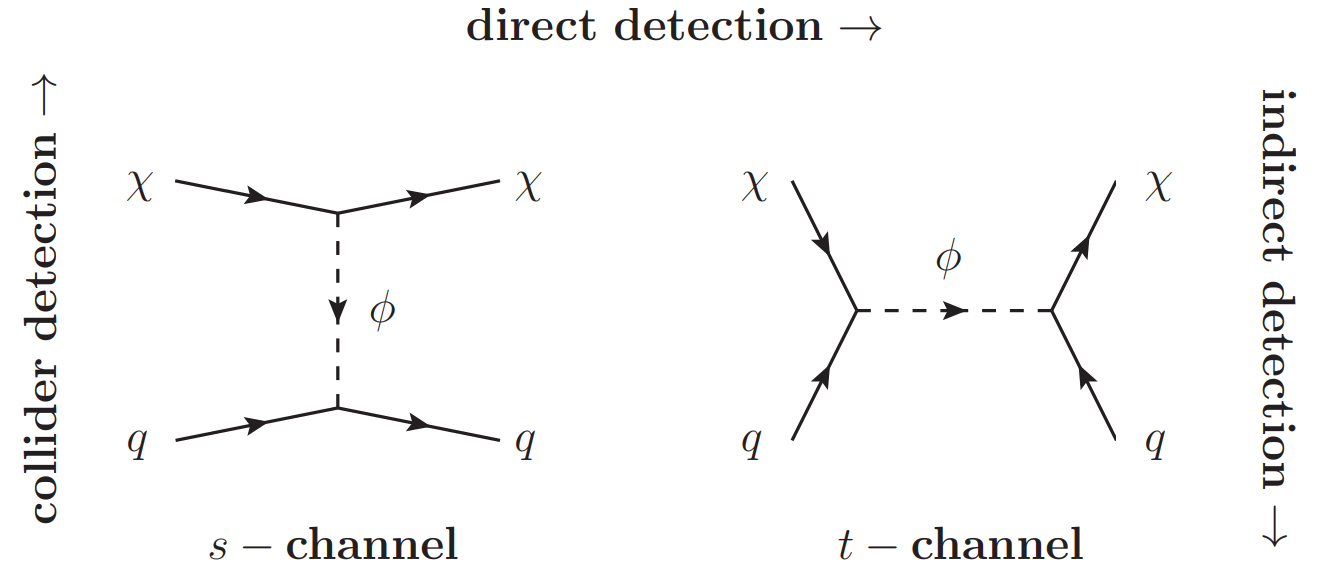
\includegraphics[width=9cm, height=4cm]{figs/STChannels.png}
\caption{Schematic representation of a typical collider \ac{DM} production through s-channel and t-channel processes \cite{STChannels}.}
\label{fig:STChannels}
\end{center}
\end{figure}

In this work, simplified models with either scalar or pseudoscalar mediators will always be considered because of their relative simplicity and the lack of strong assumptions behind them. We will now study in particular the production and the search for \ac{DM} within the \ac{LHC}.

\section{\ac{DM} production at the \ac{LHC}} \label{section:ourChannel}

The \acf{LHC}, colliding protons at a center of mass energy of 13 TeV, is actually a perfect machine to study such processes, because of the expected range of masses (100 GeV to 1 TeV) for the best \ac{DM} candidates, as discussed in Section~\ref{section:DMProperties}. However, because of the weak interactions of such particles, they are not expected to interact at all with the detector, which will then basically search for missing transverse energy along with a \ac{SM} particle triggering the event.

Several major categories of \ac{DM} searches exist at the \ac{LHC}, performed mainly by the \ac{CMS} and \ac{ATLAS} collaborations, depending on the strategy applied for such searches:

\begin{itemize}
\item First of all are the so-called \textbf{mono-X searches}, where X stands for a detectable \ac{SM} particle used to trigger the event while the \ac{DM} mediator usually decays into a pair of particles escaping the detector, leaving behind some \ac{MET}, a key variable to all these searches, as shown in Figure~\ref{fig:MonoX}. Depending on the nature of the X particle, several searches can be performed: we can for example mention the mono-$\gamma$ \cite{MonoGammaAtlas, MonoGammaCMS} or mono-jet \cite{MonoJetCMS, MonoJetCMS2} 13 TeV searches performed by the \ac{ATLAS} and \ac{CMS} collaborations.

\begin{figure}[htbp]
\begin{center}
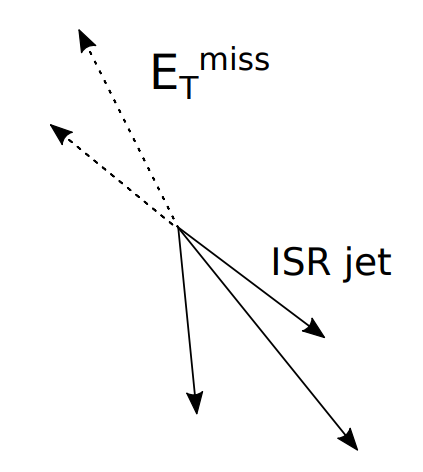
\includegraphics[width=4.5cm, height=4cm]{figs/MonoX.png}
\caption{Schematic representation of a typical mono-X event, with an \ac{ISR} jet in this case going back-to-back with some \ac{MET} \cite{ColliderSearches}.}
\label{fig:MonoX}
\end{center}
\end{figure}

Additionally, if the \ac{DM} mass is high enough, a coupling to the Higgs boson is also possible, or an eventual decay of the Higgs itself to a couple of \ac{DM} particles $H \rightarrow \chi \bar \chi$ is kinematically not impossible. This channel, known as the mono-Higgs searches is sensitive to all the decays of the Higgs, even though the searches excluding most of the phase spaces are performed using the $H \rightarrow b \bar b$ and $H \rightarrow \gamma \gamma$ decays, mainly because of their branching ratios \cite{MonoHiggsAtlas, MonoHiggsCMS}. 

\item Then. we can find the searches for \ac{DM} production in \textbf{association with heavy quark(s)}. This particular search for \ac{DM} produced in association with one or two quark pairs can be typically quoted within this category and will be detailed in the next section, but other analyses such as the one probing the $b \bar b$ + DM to its different final states depending on the decay of the bottom quark also belongs to this group, at 8 or 13 TeV \cite{PreviousDoubleTopAllLep8ATLAS, PreviousDoubleTopBottomAllLep13ATLAS}. 

These searches have to combine the discriminant power of several variables to separate the signal from the backgrounds, since the \ac{MET} distribution on its own is usually not enough, but they present the advantage of being favored by the higher Yukawa coupling to more massive particles implied by the \ac{MFV} assumption.

\item \textbf{Dijet searches} are also an important part of the work being performed using the \ac{LHC} data, and actually provide the best exclusion limits for most the spin-1 mediated models considered (up to a few TeV for typical coupling choices!) \cite{DijetAtlas, DijetCMS}. In this case, the sensitivity is obtained by searching for either narrow or large resonances on the exponentially falling QCD background, while the other searches were mostly dedicated in searching for bumps in the \ac{MET} spectrum.
\item \textbf{Supersymmetric searches}, such as SUSY searches, can also be performed to search for \ac{DM} which would solve the hierarchy problem while giving us perfect \ac{DM} candidates such as the neutralino $\chi$, the lightest stable supersymmetric particle, obtained in many of the \ac{MSSM} theories, having an hypothetical mass below the TeV scale \cite{SUSYDM}.
\item The \textbf{Higgs portal} to the dark sector is another interesting strategy. In some specific cases, when considering spin-0 mediated interactions between the dark and baryonic sectors, the Higgs could be considered as the mediator of the interaction as well, which only require a minimal modification of the \ac{SM} Lagrangian. It is then necessary to study the different Higgs production modes, such as the gluon fusion and \ac{VBF} mechanisms, to search for an eventual invisible decay of the Higgs into a couple of \ac{DM} particles, assuming that its mass is lower than $\sim 62.5$ GeV, $m_H/2$ \cite{InvisibleHiggs}.
\item Finally, and this is quite new, \textbf{long-lived searches} can also be performed. These are interested because they can extend the current searches performed to also consider the eventual creation of long-lived particles which would decay a few centimeters further than the primary vertex of the proton-proton collision \cite{LLSearches}. Typical \ac{SM} signatures do not usually include such events, making this channel relatively background-free, even though the reconstruction of the different objects is much harder in this case.
\end{itemize}

All the results obtained the different searches performed by the \ac{CMS} collaboration using the full 2016 dataset can be summarized in Figure~\ref{fig:SummarySpin0} for spin-0 mediators and in Figure~\ref{fig:SummarySpin1} when considering spin-1 mediators.

\begin{figure}[htbp]
\centering
\begin{minipage}[b]{.47\textwidth}
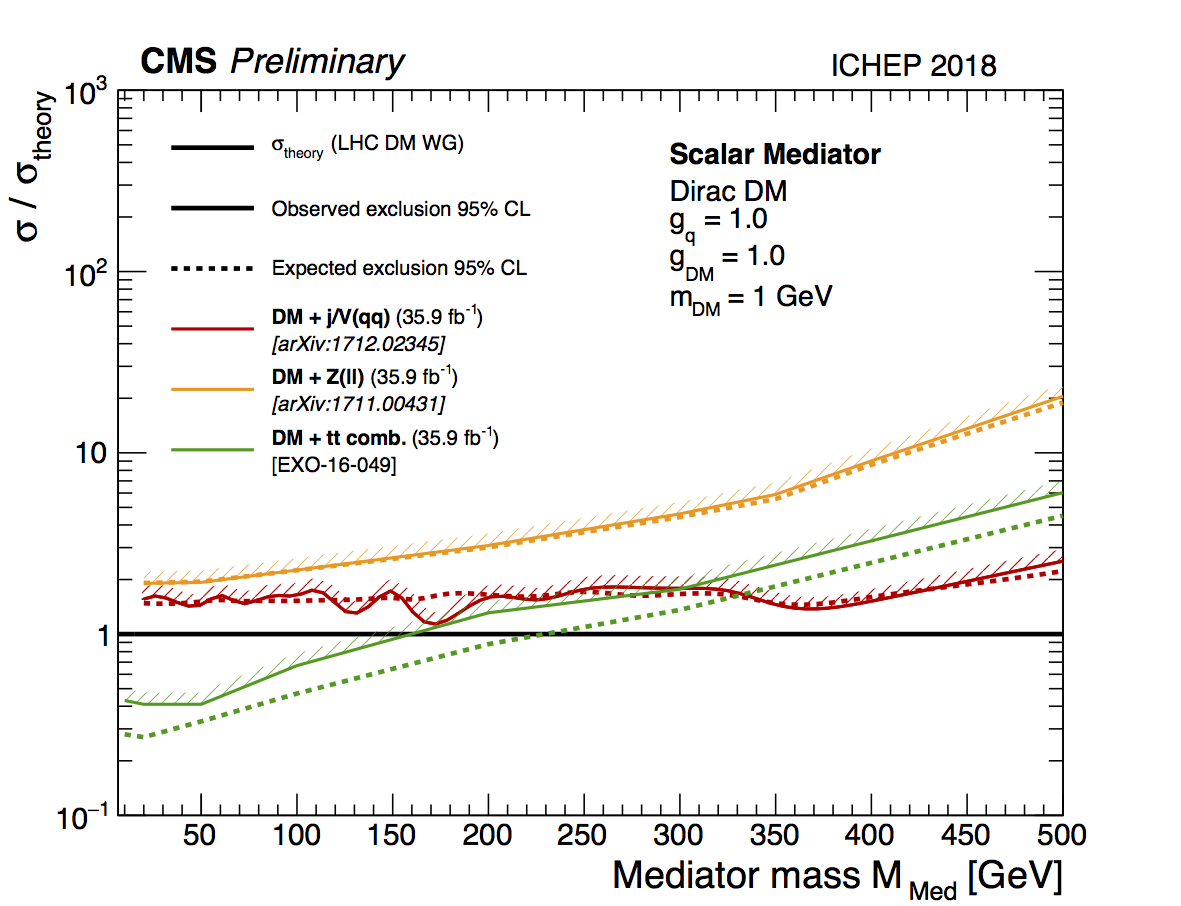
\includegraphics[width=8cm, height=7cm]{figs/SummaryScalar.png}
\end{minipage}\hfill
\begin{minipage}[b]{.47\textwidth}
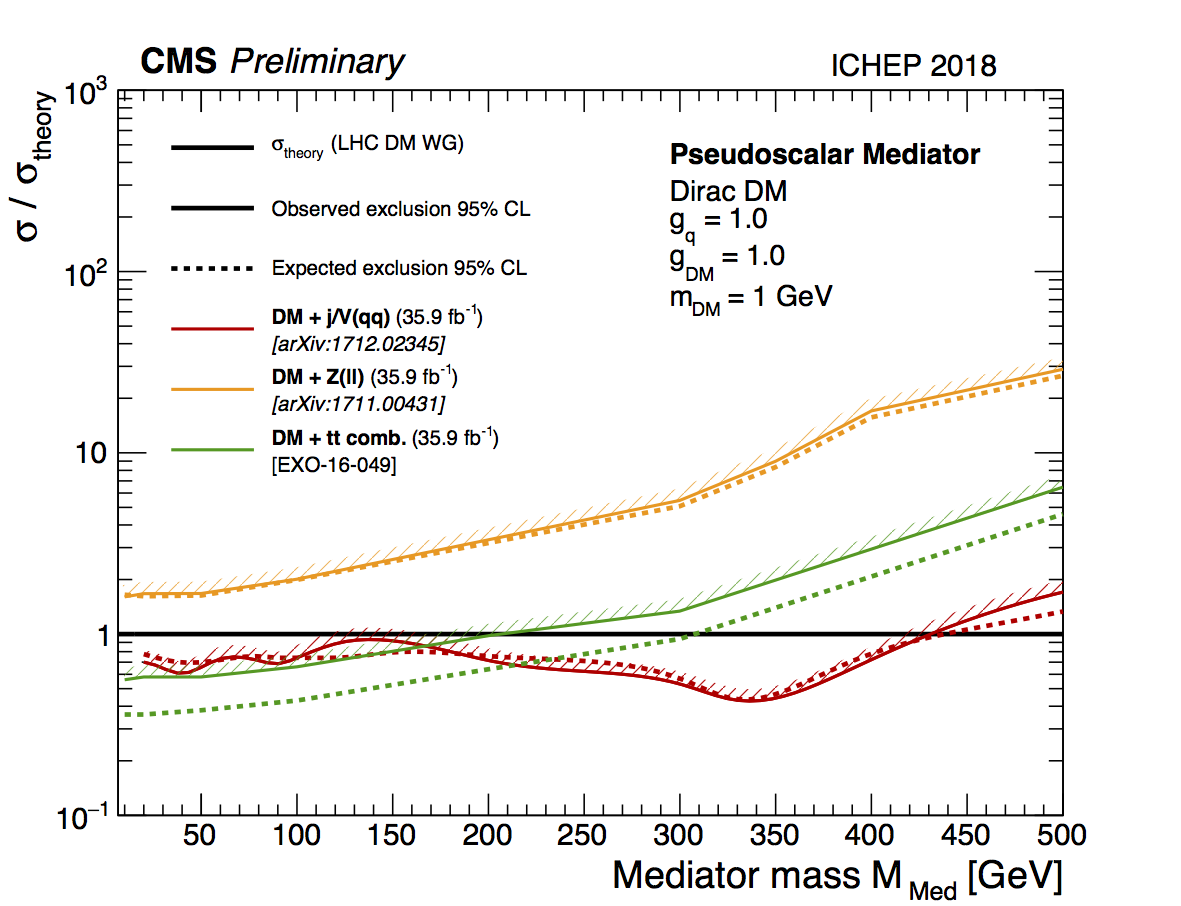
\includegraphics[width=8cm, height=7cm]{figs/SummaryPseudoScalar.png}
\end{minipage} \hfill
\caption{Observed and expected 95\% exclusion limits obtained by different searches of the \ac{CMS} collaboration as a function the spin-0 scalar (on the left) or pseudoscalar (on the right) mediator.}
\label{fig:SummarySpin0}
\end{figure}

\begin{figure}[htbp]
\centering
\begin{minipage}[b]{.47\textwidth}
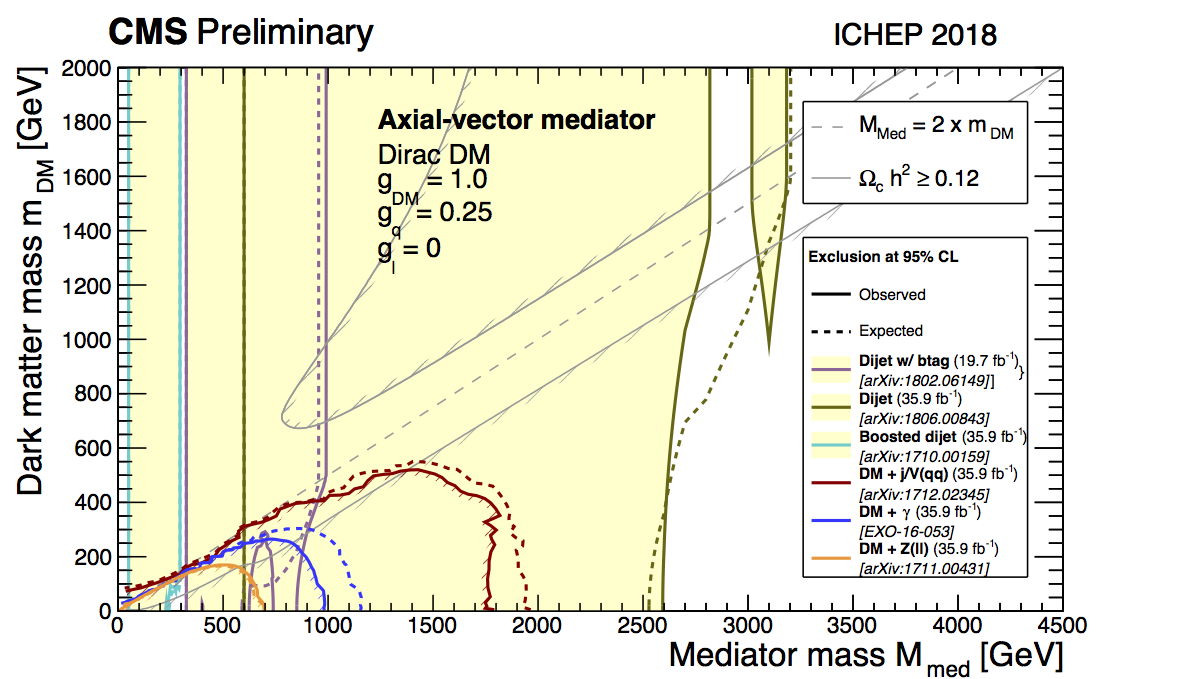
\includegraphics[width=8.5cm, height=5.5cm]{figs/SummaryAxialVector.png}
\end{minipage}\hfill
\begin{minipage}[b]{.47\textwidth}
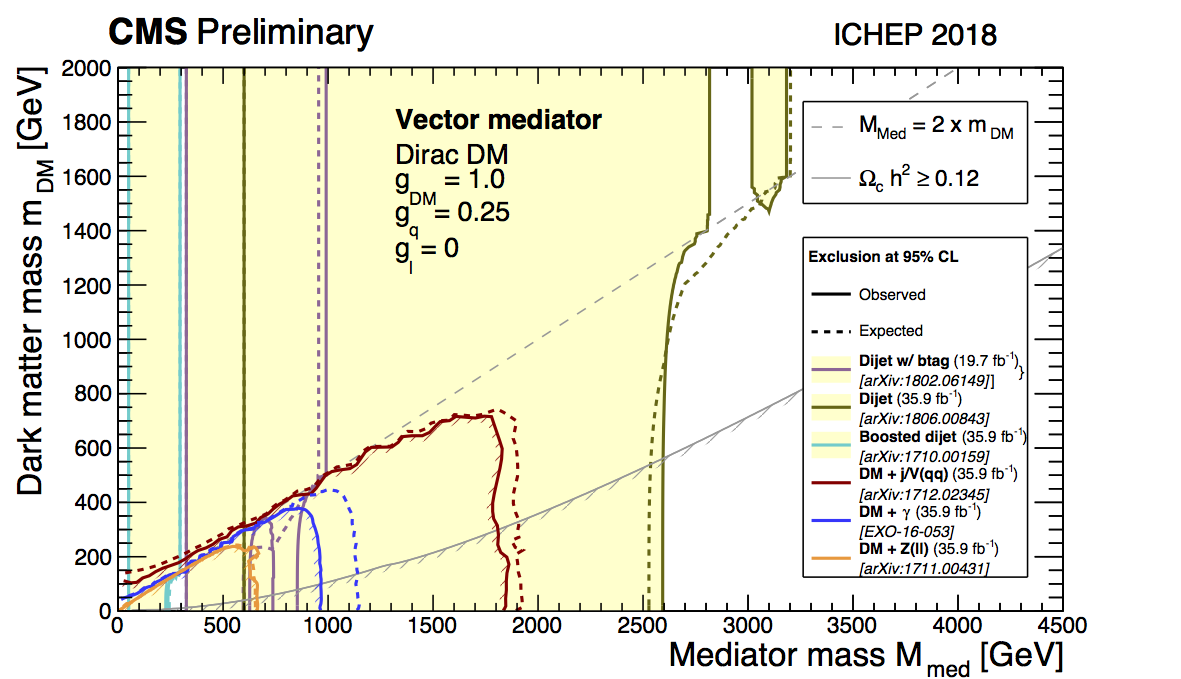
\includegraphics[width=8.5cm, height=5.5cm]{figs/SummaryVector.png}
\end{minipage} \hfill
\caption{Observed and expected 95\% exclusion limits obtained by different searches of the \ac{CMS} collaboration as a function the spin-1 mediator, considering an axial-vector (on the left) and axial (on the right) interaction.}
\label{fig:SummarySpin1}
\end{figure}

These results have also been compared to the results obtained by several direct detection experiments in Figure~\ref{fig:DDComparison}, considering both the \acf{SD} and \acf{SI} cases, as explained in Section~\ref{subsection:DirectSearches}.

\begin{figure}[htbp]
\centering
\begin{minipage}[b]{.47\textwidth}
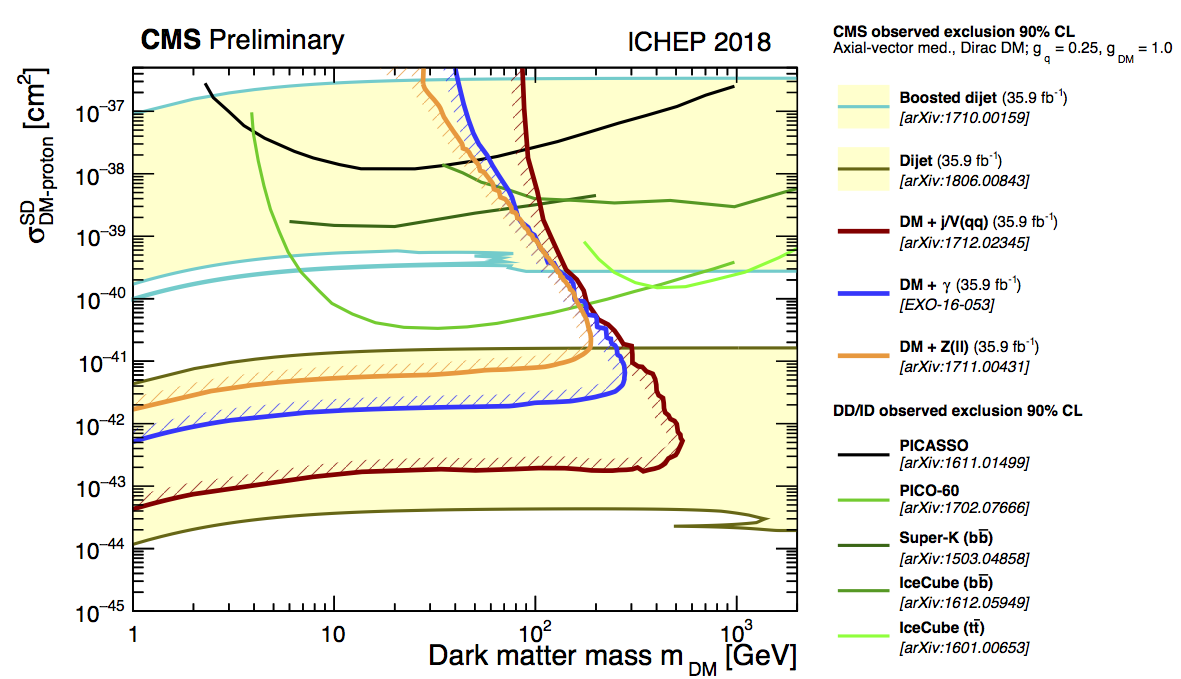
\includegraphics[width=8.5cm, height=5.4cm]{figs/SDDD.png}
\end{minipage}\hfill
\begin{minipage}[b]{.47\textwidth}
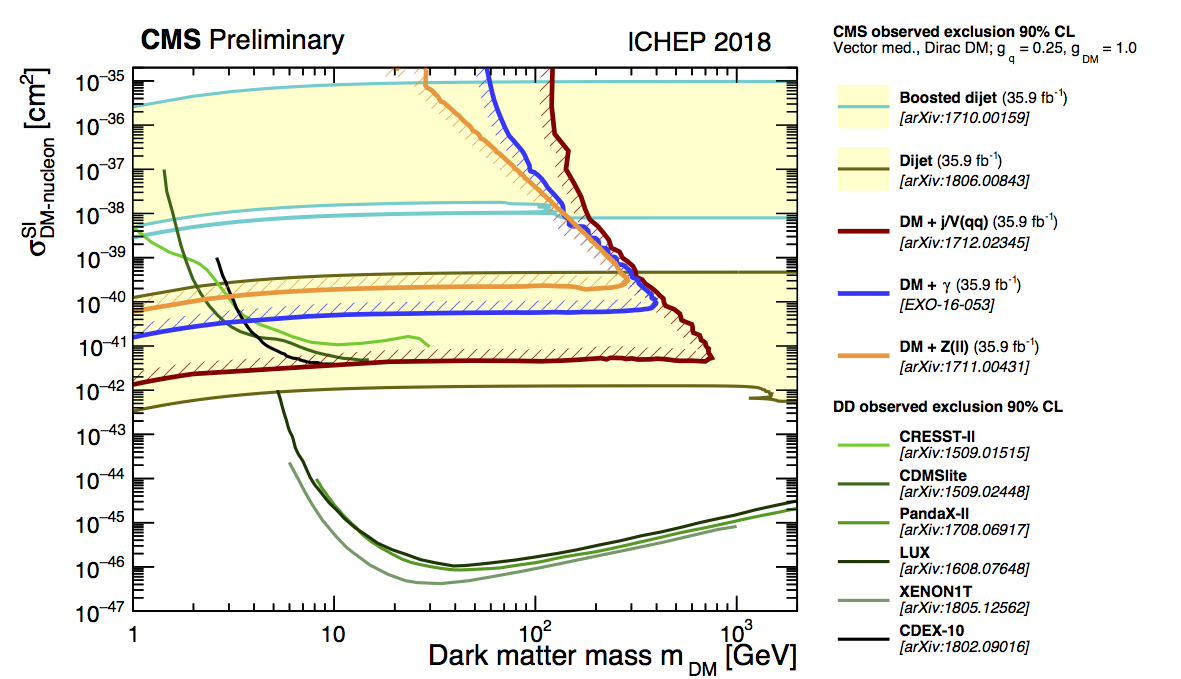
\includegraphics[width=8.5cm, height=5.4cm]{figs/SIDD.png}
\end{minipage} \hfill
\caption{\ac{CMS} 90\% exclusion limits compared to the most famous direct detection experiments for the \ac{SD} (on the left) and \ac{SI} (on the right) scenarios, obtained using similar couplings.}
\label{fig:DDComparison}
\end{figure}

This particular analysis and our signal of interest, the search for \ac{DM} production in addition with a single or a pair of top quarks falls into the second category and will now be detailed. It is already important to note that this analysis has been performed considering the \ac{DM} candidate to be a 1 GeV Dirac fermion with all the couplings equal and set to 1, as recommended by the \ac{DMWG} \cite{DMWG}.

\subsection{The single top production channel} \label{subsection:singleTopChannel}

The first kind of signal considered in this analysis is the production of \ac{DM} in association with a single top quark, known as $t/\bar t$+DM analysis. This process is expected to be mediated by a spin-0 mediator, either scalar or pseudoscalar, and is associated with a light quark and a W boson (the mono-top analysis is dealing with the case where a single top is created without any additional particle). 

Three different Feynman diagrams can be associated to this particular analysis depending on the model considered, as shown in Figure~\ref{fig:singleTopFeynman}.

\begin{figure}[htbp]
\centering
\begin{minipage}[b]{.3\textwidth}
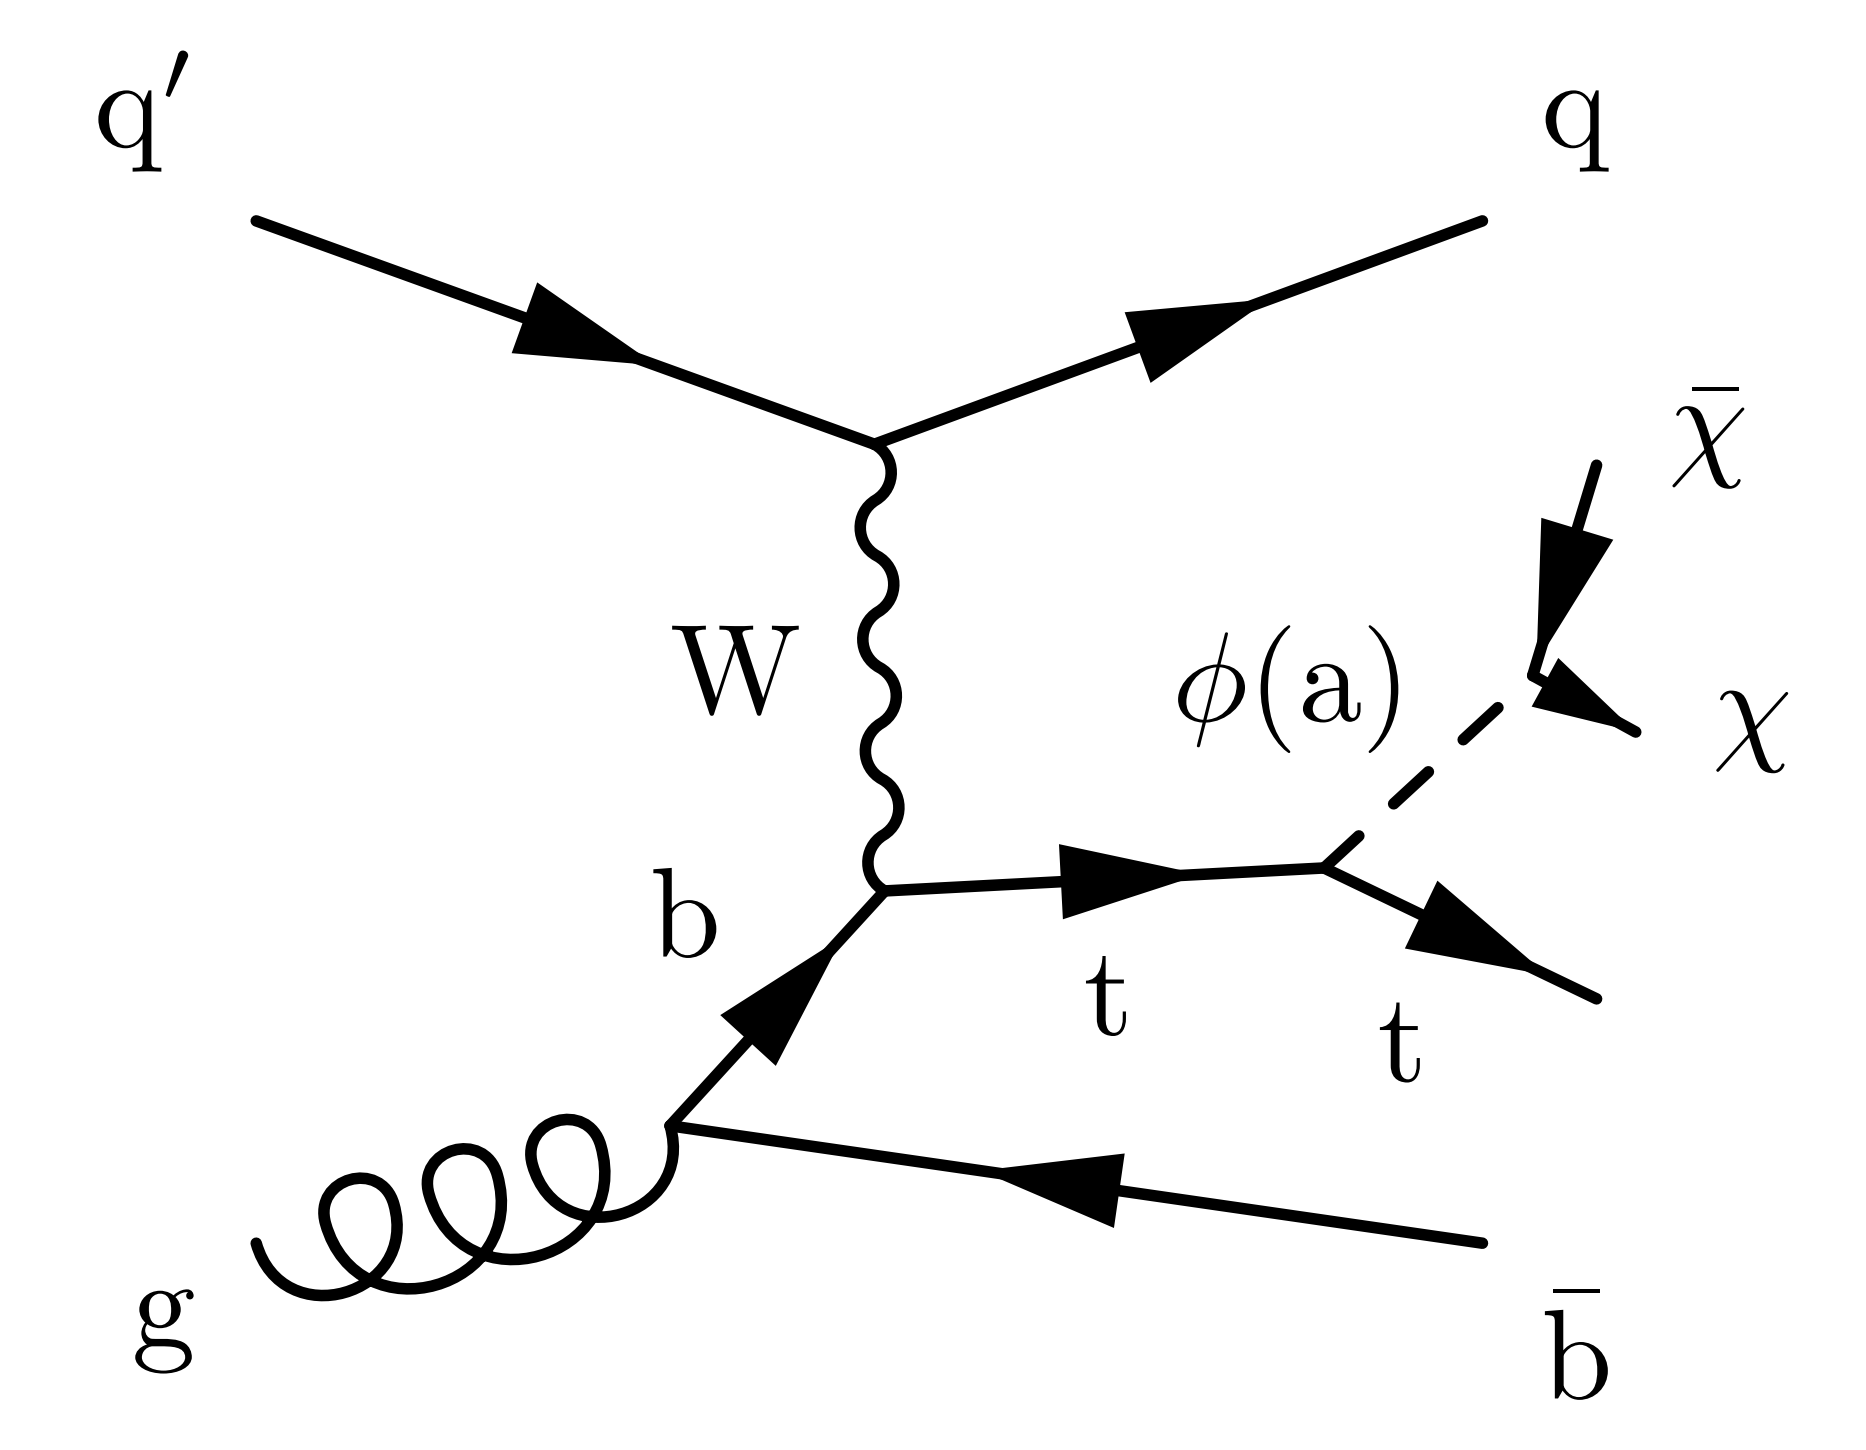
\includegraphics[width=4.8cm, height=3.5cm]{figs/tDMa.png}
\end{minipage}\qquad
\begin{minipage}[b]{.3\textwidth}
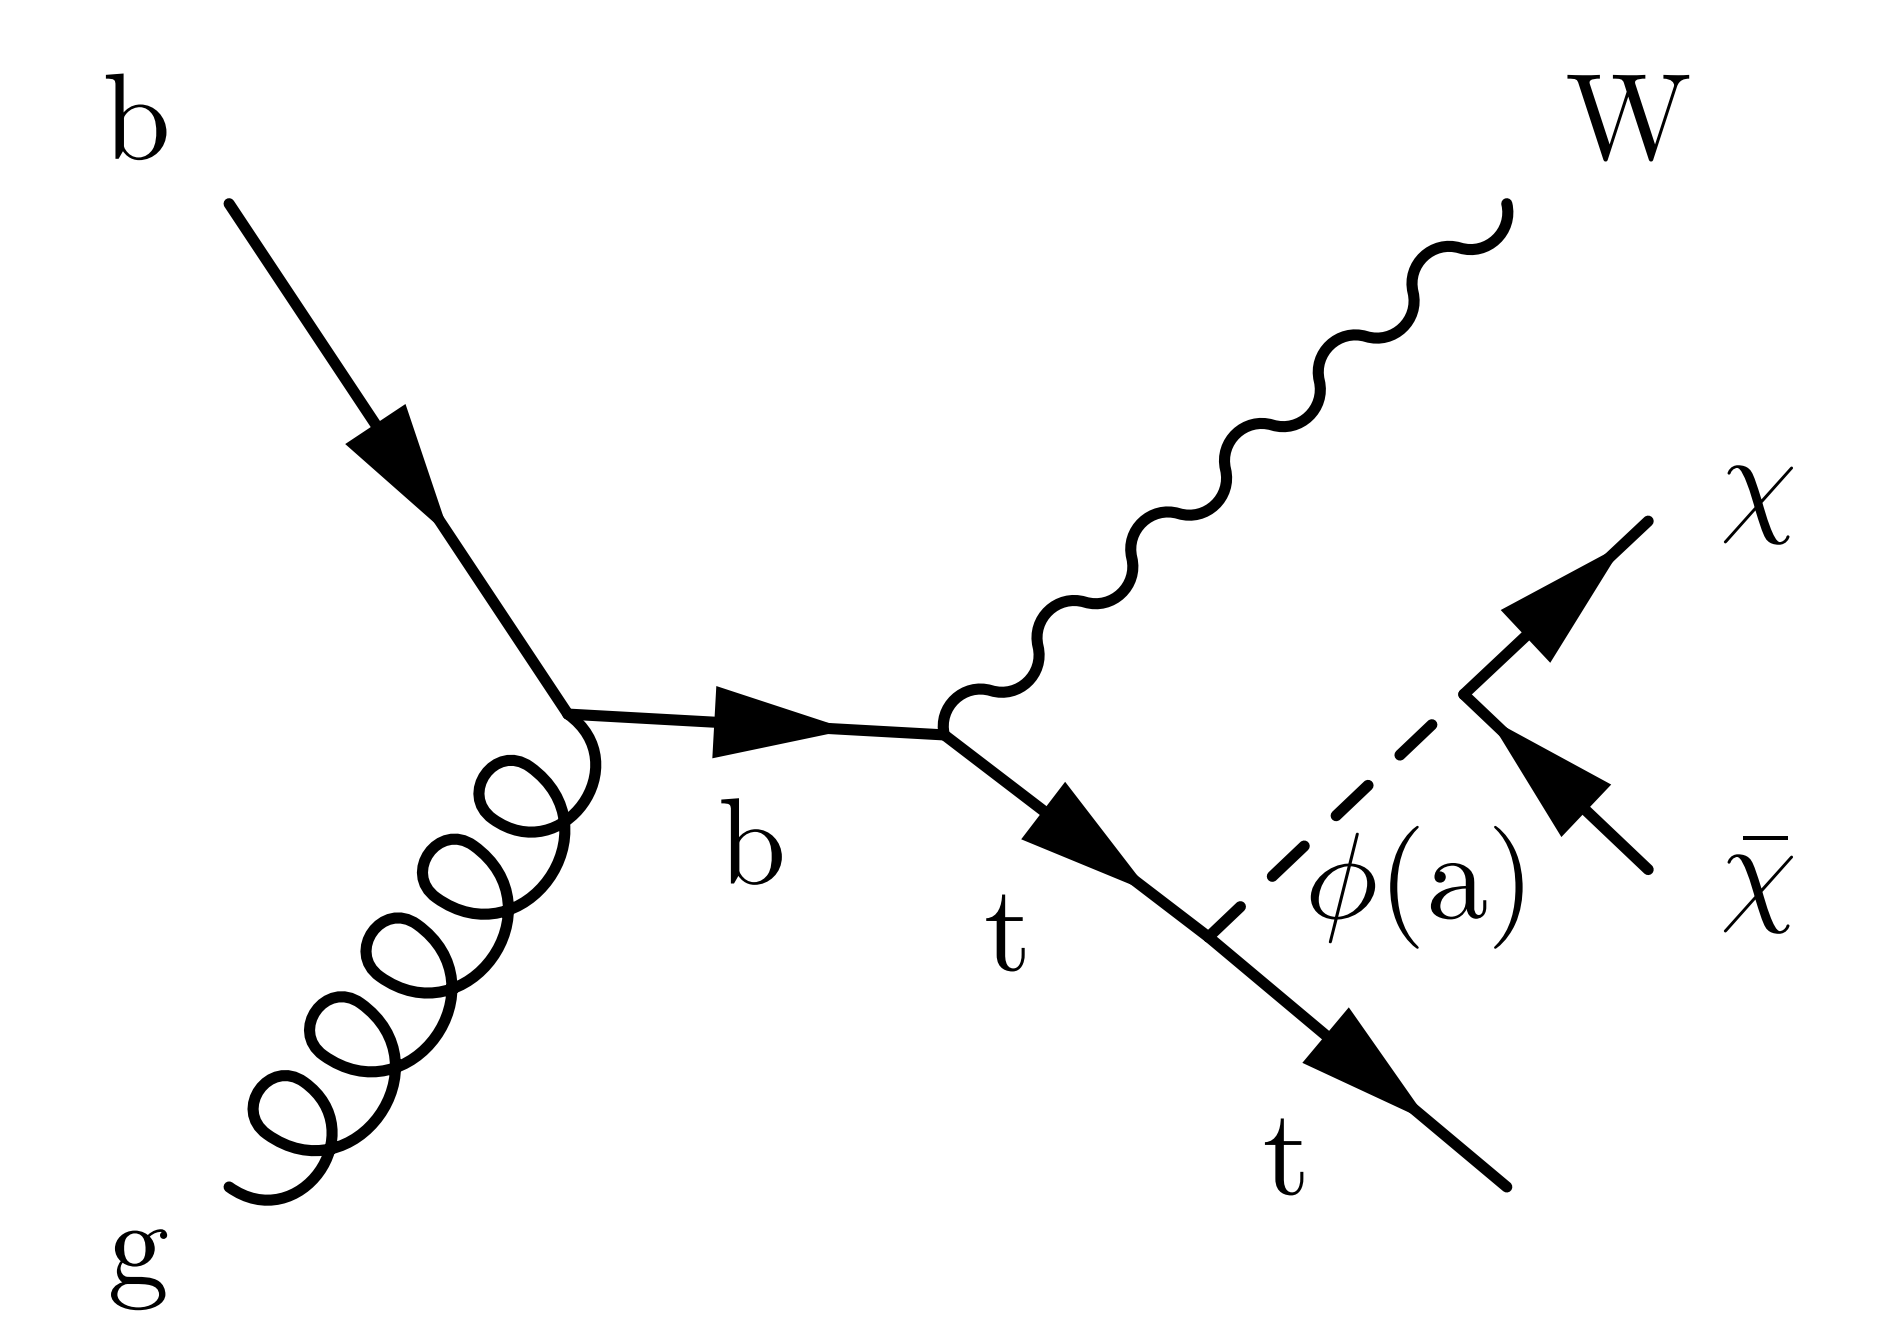
\includegraphics[width=4.8cm, height=3.5cm]{figs/tDMb.png}
\end{minipage}
\begin{minipage}[b]{.28\textwidth}
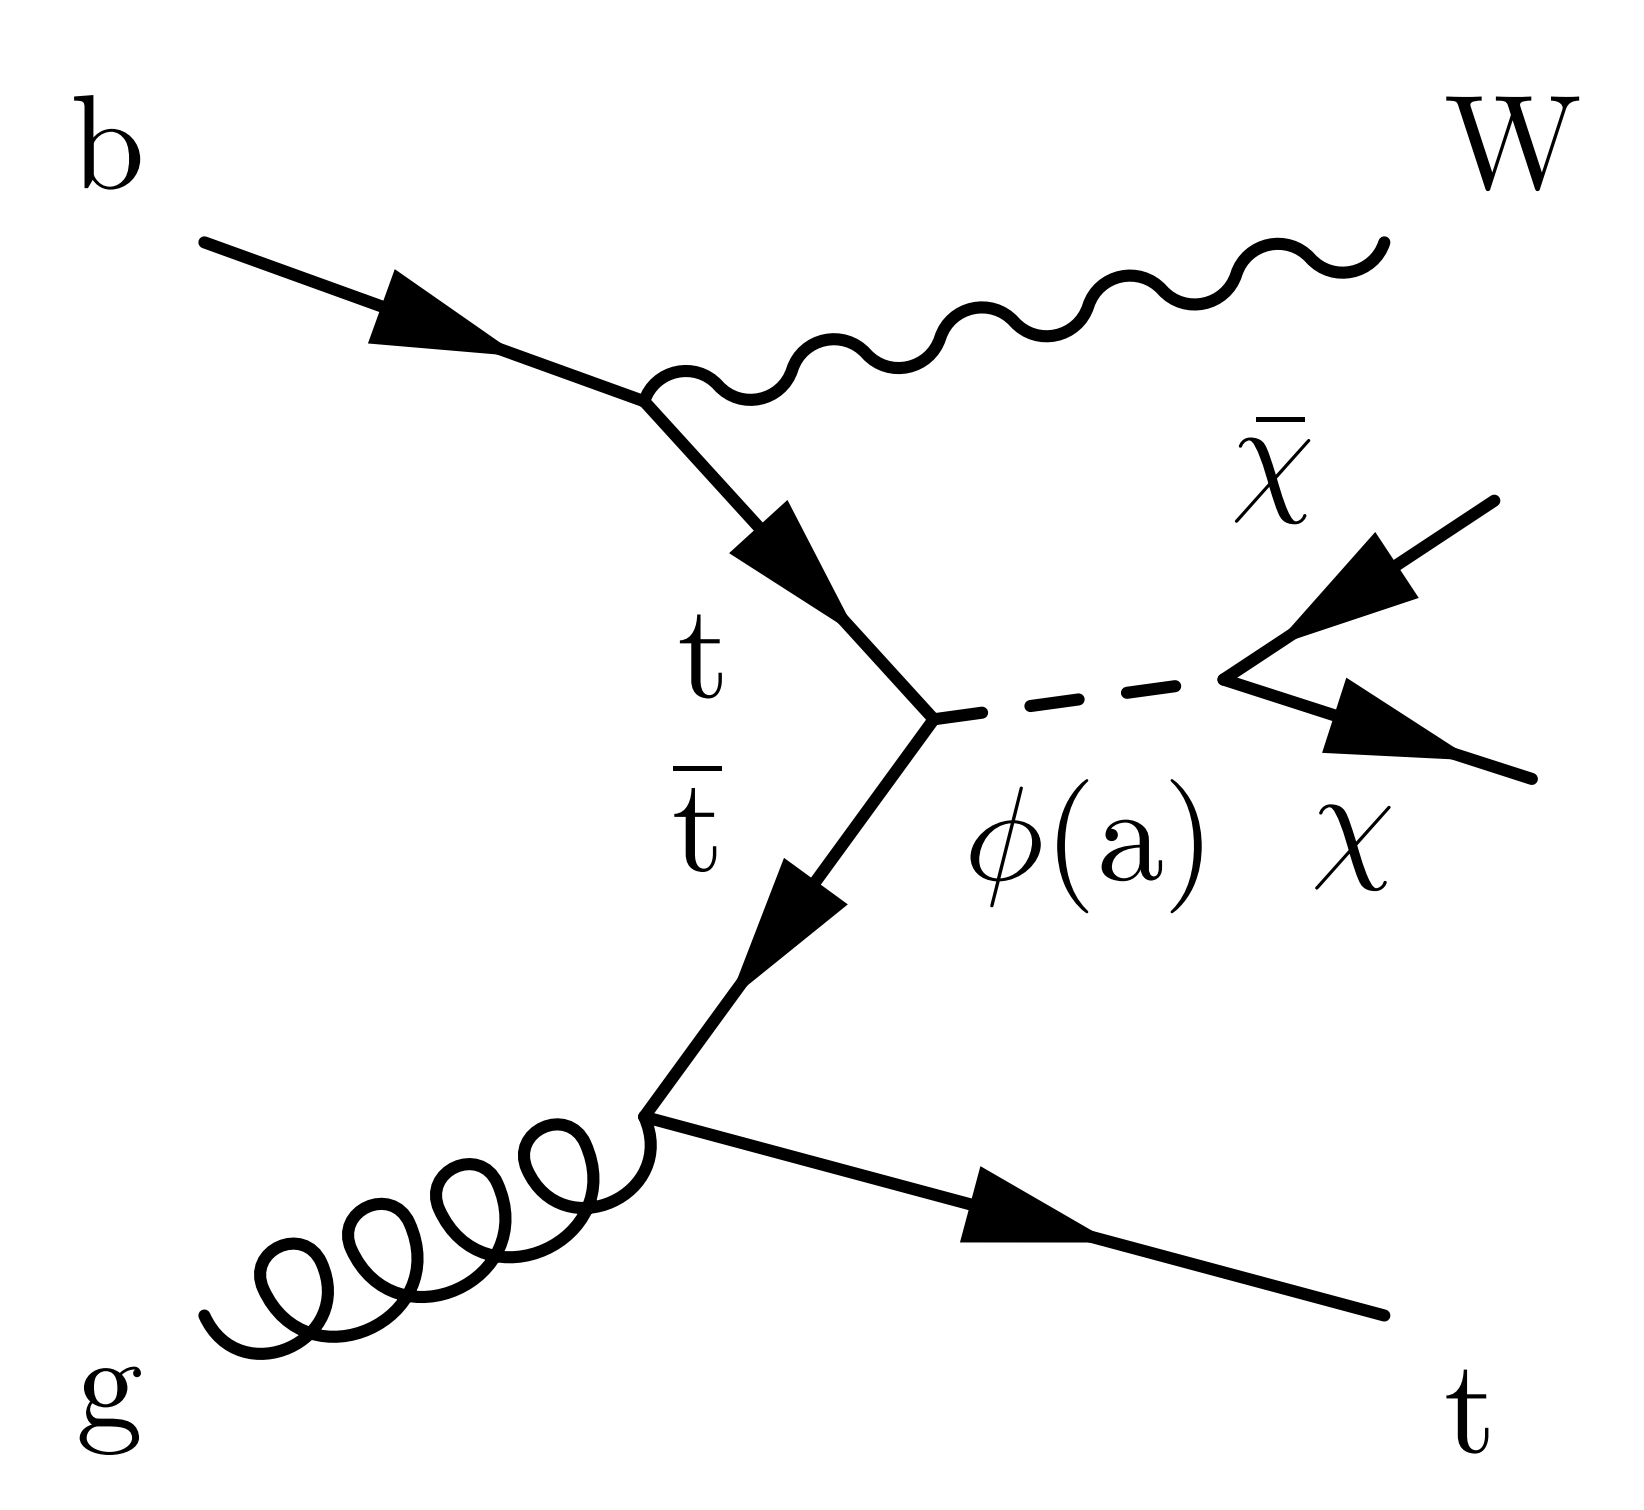
\includegraphics[width=4.8cm, height=3.5cm]{figs/tDMc.png}
\end{minipage}
\caption{Feynman diagrams involving the production of \ac{DM} with a single top quark with its associated t-channel W boson (on the left), or tW (on the center and on the right) production.}
\label{fig:singleTopFeynman}
\end{figure}

As discussed previously, the top quark will be dynamically favored due to its high mass and therefore high Yukawa coupling, but however this has a negative effect as well, since the lifetime of this quark is extremely low, of the order of $10^{-15}$ s \cite{PDG}. This means that this particle usually decays before being able to form hadrons and before reaching the \ac{CMS} detector, so we can only detect the products of its decay, not he top quark itself. In almost 100\% of the cases, the top actually decays into a bottom quark and a W boson, which decays itself before being detected into quarks and/or leptons. Even though this will de detailed in Chapter~\ref{chapter:Selection}, we can already conclude that the typical final state of such signature is therefore made out of \ac{MET} coming from the \ac{DM}, one b-tagged jet along with one or two W bosons, seen as a combination of jets and leptons, depending on the channel considered.

\subsection{The $t \bar t$ production channel} \label{subsection:ttChannel}

The $t \bar t$+DM analysis is really similar, except that in this case, we have two top quarks in the final state, as represented in Figure~\ref{fig:ttDMFeynman}.

\begin{figure}[htbp]
\begin{center}
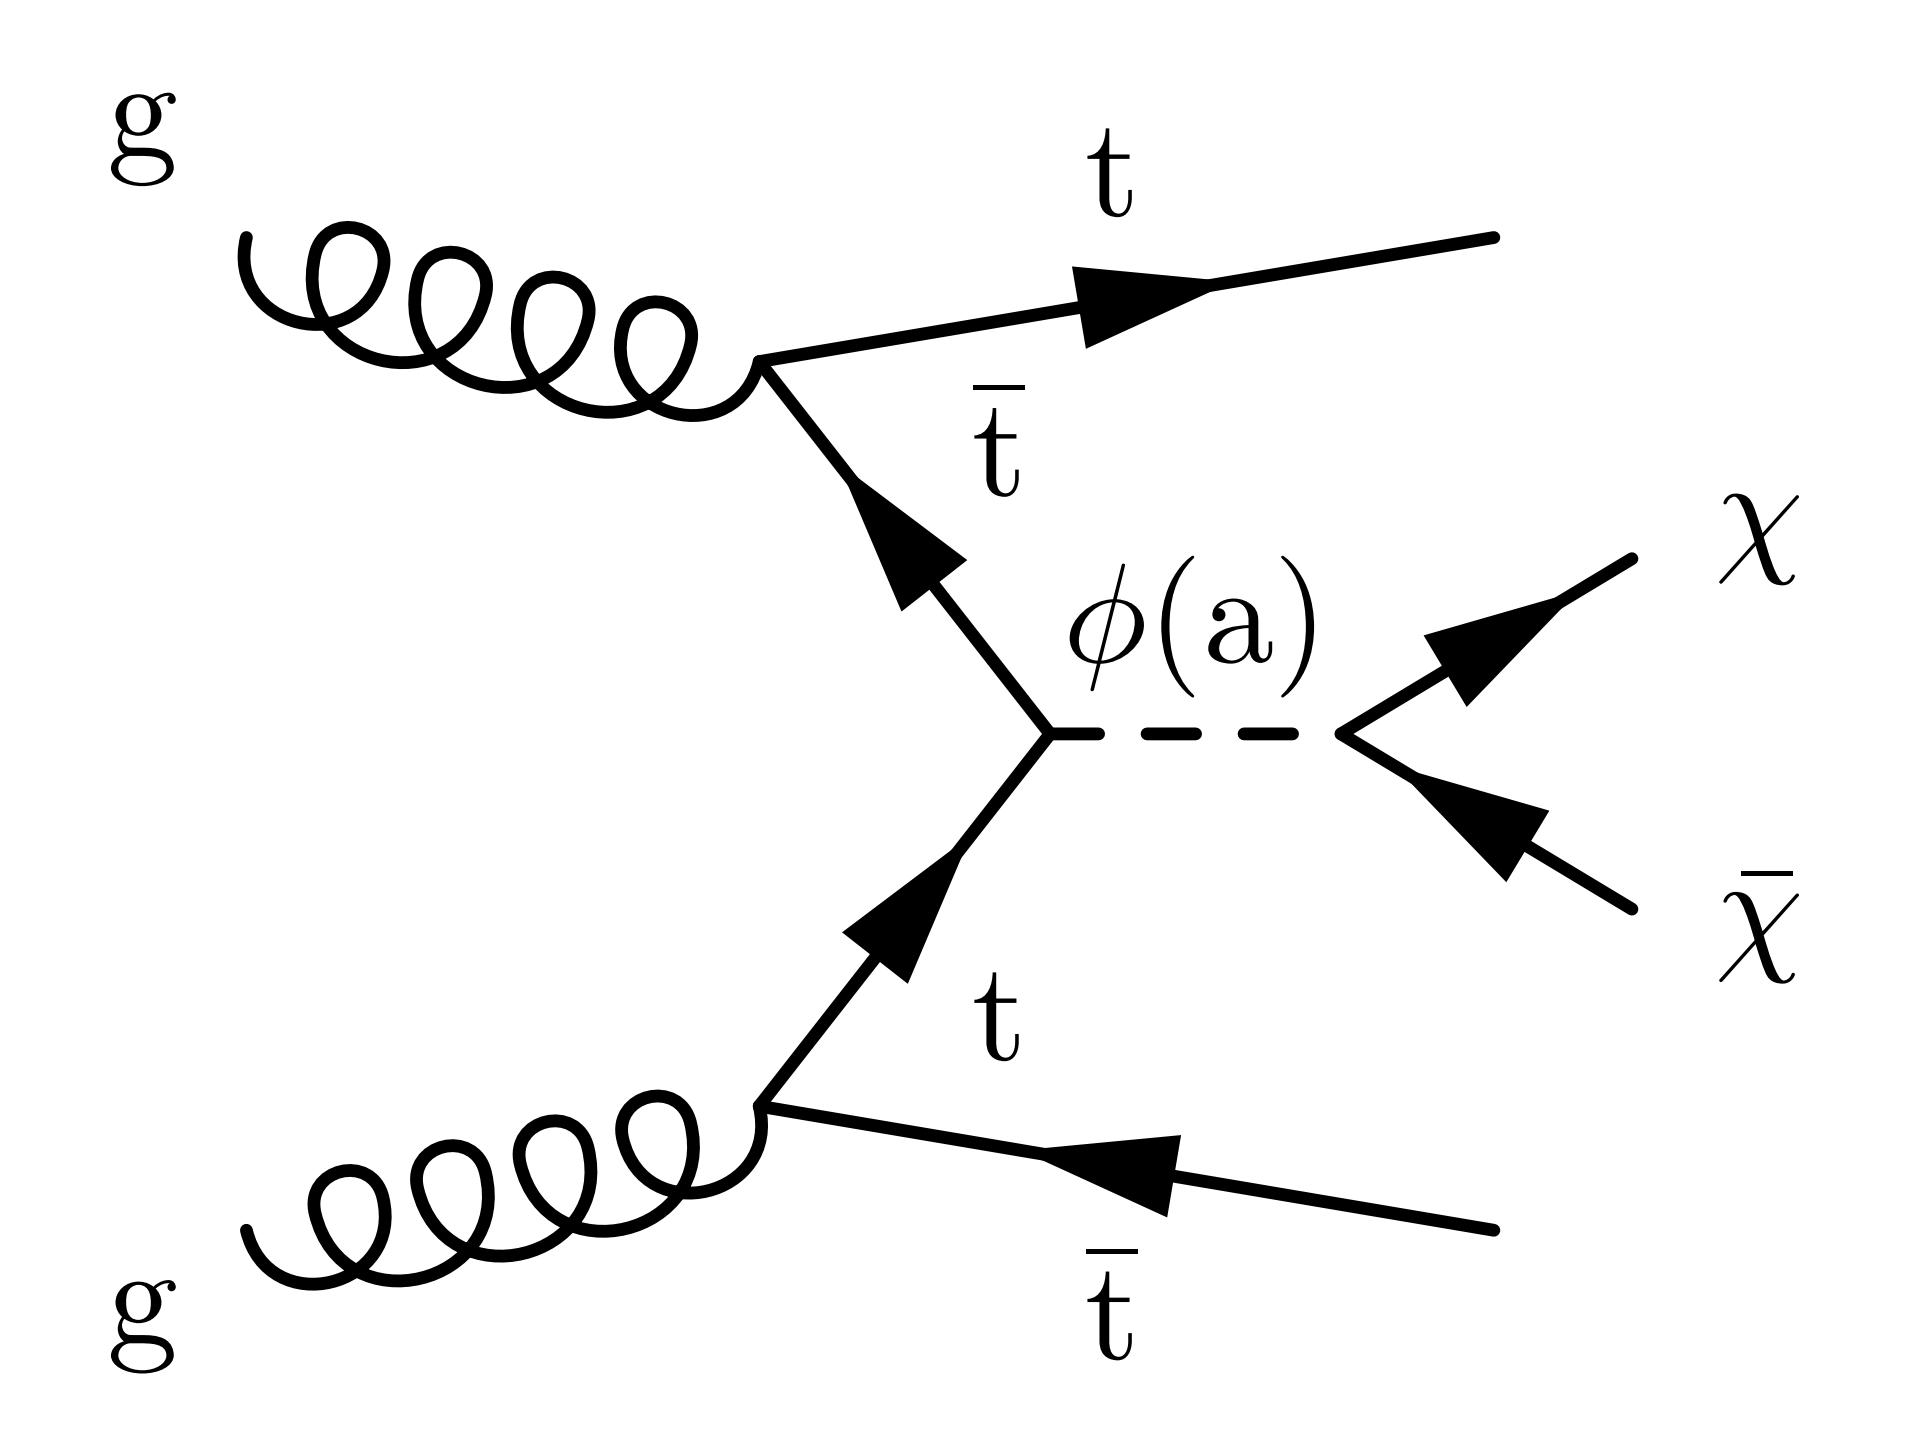
\includegraphics[width=4.5cm, height=3.5cm]{figs/ttDM.png}
\caption{Schematic representation of a typical $t \bar t$+DM event.}
\label{fig:ttDMFeynman}
\end{center}
\end{figure}

The final state expected by such an event is therefore made of two b-tagged jets, along with two W bosons and some \ac{MET} coming from the pair of \ac{DM} particles as well. In this case as well, both scalar $\phi$ and pseudoscalar $a$ mediators will be considered as well, with a mass range from 10 to 500 GeV.

\subsection{The dilepton final state} \label{subsection:diLeptonFS}

As previously explained, most of the models considered will produce exactly two W bosons, which are not stable long enough and therefore decay before reaching the detector, meaning that we cannot directly detect such bosons. However, we can detect the results of the decays of these W, since they can decay either to hadrons ($67.6 \pm 0.27 \%$ branching ratio) or to a lepton and a neutrino, giving us an additional contribution of \ac{MET} ($10.8 \pm 0.09 \%$) \cite{PDG}.

This means that this kind of analyses featuring two W bosons in the final state can focus on different channels: either completely hadronic (if both the W decay into quarks), semileptonic or dileptonic (when both the W decay into two neutrinos and two leptons of opposite charge). 

Given the \ac{BR} of the W decay, it is easy to see that the dileptonic channel, which will be the focus of this work, is clearly not favored statistically. However, it is interesting anyway to study this kind of decay because this channel typically features less backgrounds than other channels, resulting in a better signal isolation, and because leptons can usually be reconstructed in a better way than jets (cf. Chapter~\ref{chapter:Reco}), resulting in lower uncertainties and in improved limits.

\section{Previous relevant results} \label{section:PreviousResults}

This analysis being performed at a center of mass energy $\sqrt{s} = 13$ TeV, only the most relevant results to this particular energy and previously obtained by both the \ac{CMS} and \ac{ATLAS} collaborations of \ac{CERN} will be quoted here. 

First of all, the \textbf{\ac{ATLAS} collaboration} published interesting results at this center of mass energy, considering an integrated luminosity of 13.3 fb${-1}$, and obtained the corresponding exclusion limits at the 95\% \ac{CL}, considering the $t \bar t$+DM model and both scalar and pseudoscalar spin-0 mediators for the interaction, as shown in Figure~\ref{fig:ATLAS13}. In this case, and for the couplings considered, an exclusion up to $\sim 375$ GeV has been achieved.

\begin{figure}[htbp]
\begin{center}
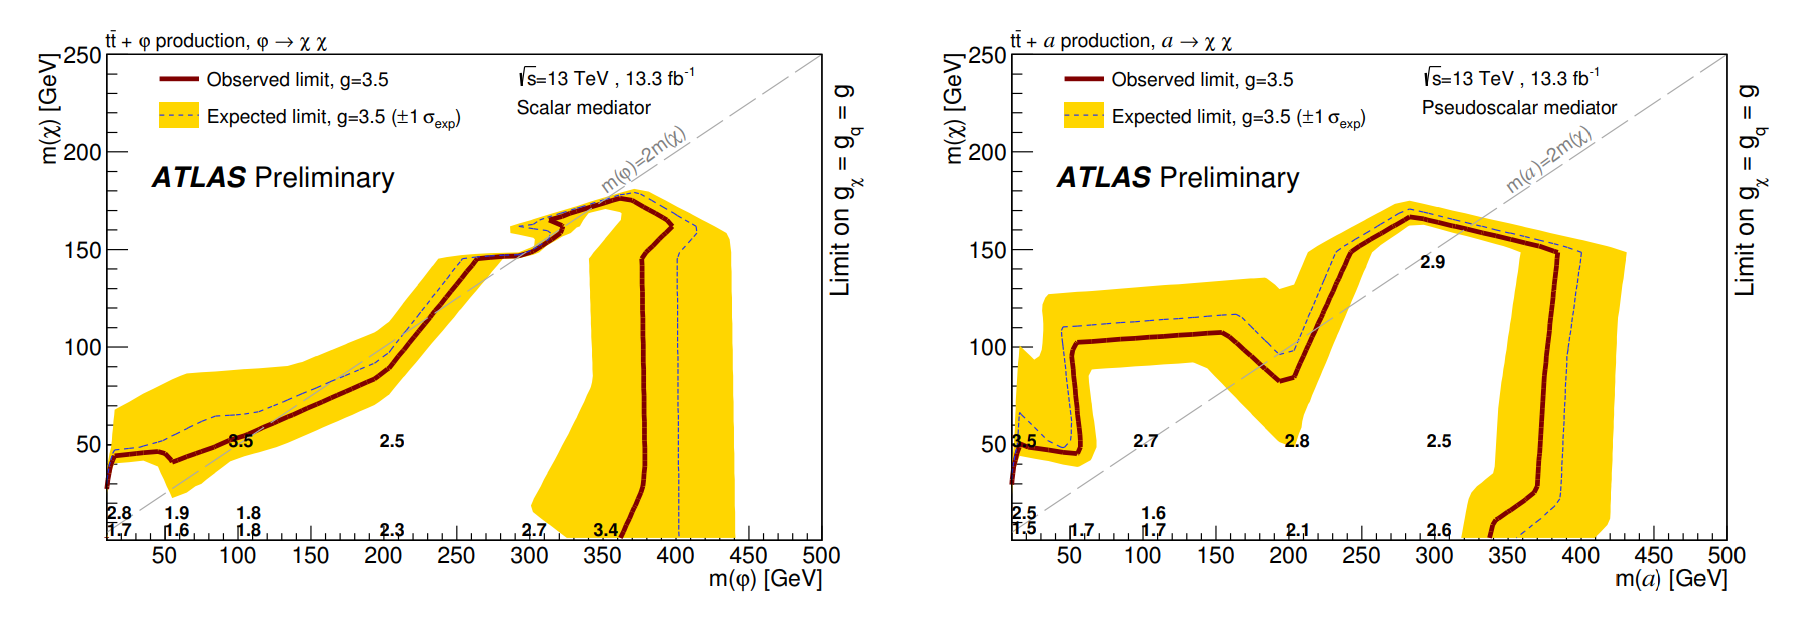
\includegraphics[width=14cm, height=6cm]{figs/Atlasttbar13fb.png}
\caption{Limits on the mass on the \ac{DM} and mediator masses obtained by \ac{ATLAS} using 13.3 fb$^{-1}$ of 13 TeV data, considering scalar (on the left) and pseudoscalar (on the right) mediators \cite{PreviousDoubleTopNoLep13ATLAS}.}
\label{fig:ATLAS13}
\end{center}
\end{figure}

Considering the full 2016 dataset of $36.1$ fb$^{-1}$, similar results have been obtained, as shown in Figure~\ref{fig:atlas36}. In this case, and for lower coupling values, an exclusion up to around 100 GeV has been obtained considering scalar and pseudoscalar mediators.

\begin{figure}[htbp]
\centering
\begin{minipage}[b]{.4\textwidth}
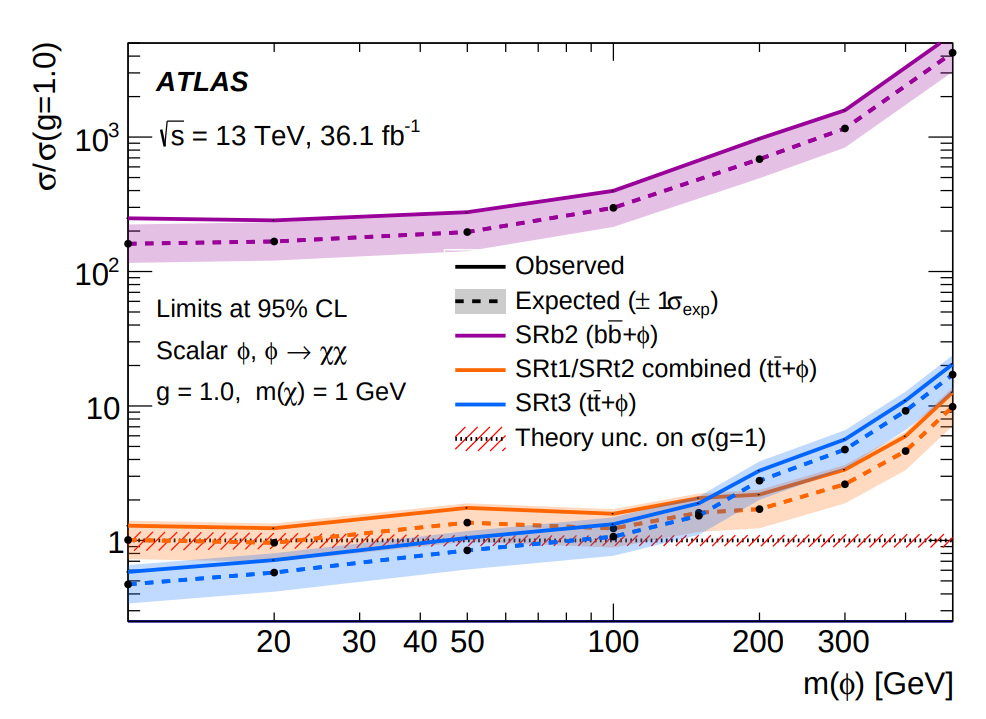
\includegraphics[width=7cm, height=6cm]{figs/Atlas36a.png}
\end{minipage}\hfill
\begin{minipage}[b]{.48\textwidth}
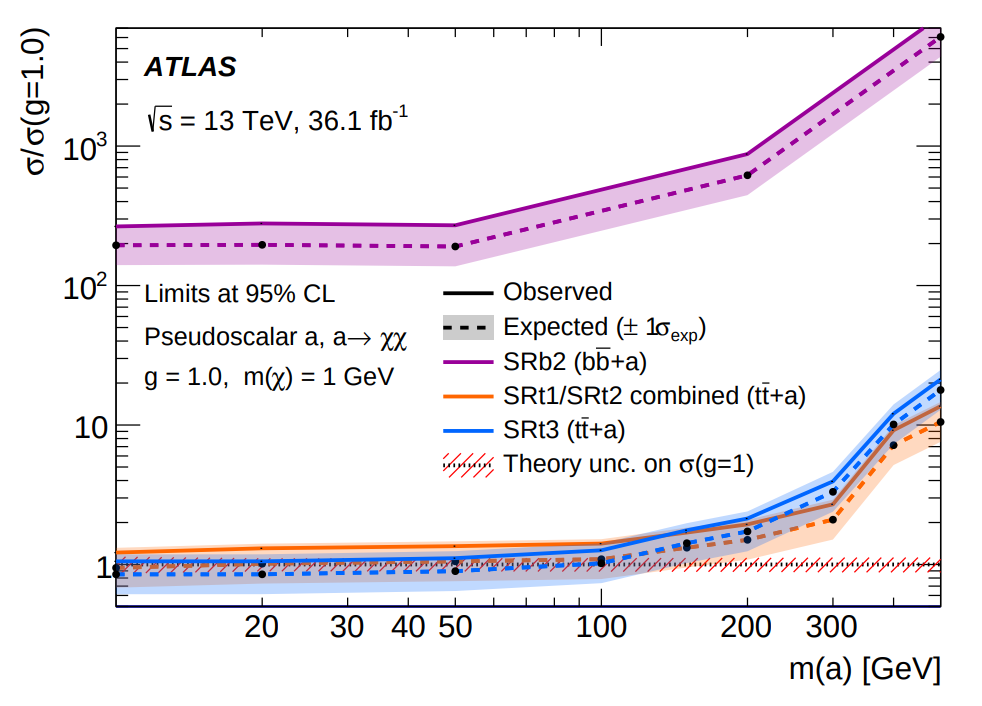
\includegraphics[width=7cm, height=5.88cm]{figs/Atlas36b.png}
\end{minipage}\hfill
\caption{Exclusion limits at the 95\% \ac{CL} obtained by \ac{ATLAS} considering  scalar (on the left) and pseudoscalar (on the right) mediators, for a \ac{DM} mass of 1 GeV \cite{PreviousDoubleTopBottomAllLep13ATLAS}}\label{fig:atlas36}
\end{figure}


The \textbf{\ac{CMS} collaboration} published in 2018 a similar analysis, but using only the $35.9$ fb$^{-1}$ of data collected during the year 2016. This analysis combined the three different final states possible (hadronic, semileptonic and dileptonic) and computed the limits on the signal strength for different mediator and dark matter masses, considering both scalar and pseudoscalar mediators \cite{PreviousDoubleTopAllLep13CMS}. The results obtained can be found in Figure~\ref{figure:CMSttbarExclusion}. 

\begin{figure}[htbp]
\begin{center}
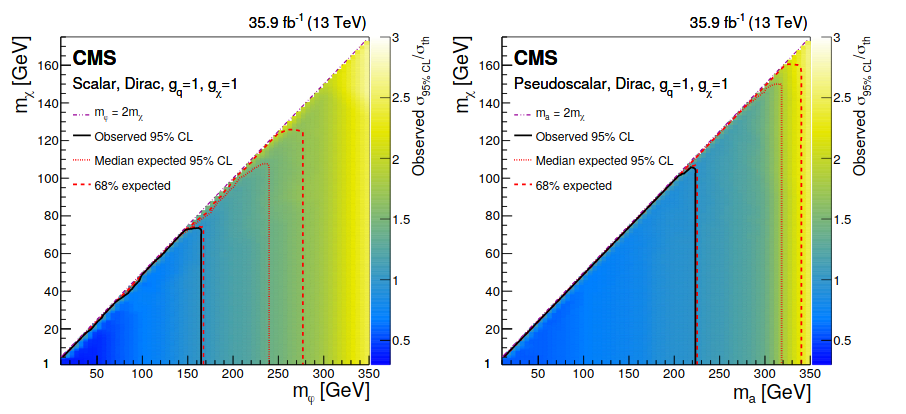
\includegraphics[width=14cm, height=6cm]{figs/CMSttbarExclusion.png}
\caption{95\% \ac{CL} exclusion plots on the signal strength computed as a function of the mediator and \ac{DM} masses obtained by \ac{CMS} considering a scalar (on the left) and a pseudoscalar (on the right) mediator for the interaction \cite{PreviousDoubleTopAllLep13CMS}.}
\label{figure:CMSttbarExclusion}
\end{center}
\end{figure}

Last year, a combination of the $t/\bar t$+DM and $t \bar t$+DM analyses has also been published \cite{PreviousSingleDoubleTopAllLep13CMS}, combining this time only the hadronic and semileptonic channels of both analyses. The limits obtained in this case are represented in Figure~\ref{figure:Combination2019}, where the limits obtained by each analysis on their own along with the results of the combination, leading to a factor 2 improvement of the limits obtained, have been represented. 

This combination managed to exclude the production of scalar mediators up to 290 GeV and pseudoscalar mediators up to 300 GeV, at the 95\% \ac{CL} for the couplings considered. This combined analysis actually lead to the most stringent exclusion limits of the \ac{LHC} on the production of \ac{DM} through these categories of spin-0 mediators.

\begin{figure}[htbp]
\begin{center}
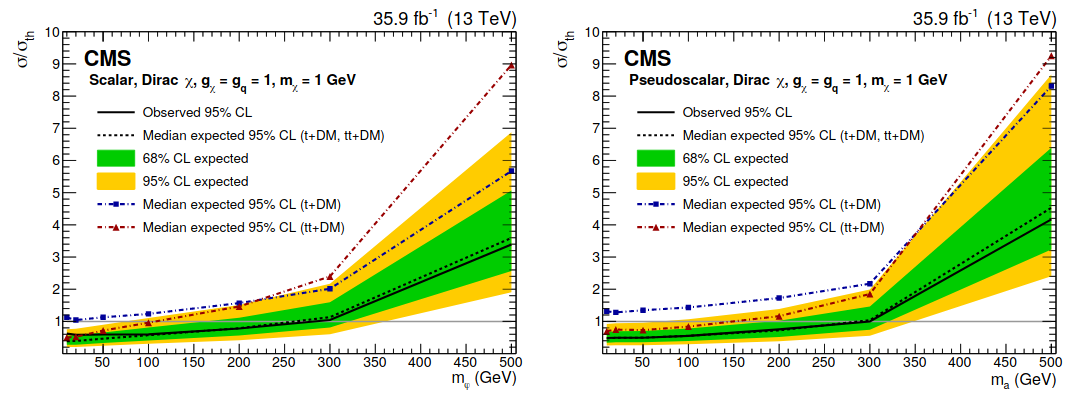
\includegraphics[width=14cm, height=6cm]{figs/Combination2019.png}
\caption{Expected and observed 95\% \ac{CL} limits on the \ac{DM} production cross sections shown considering scalar (on the left) and pseudoscalar (on the right) mediators for the interaction \cite{PreviousSingleDoubleTopAllLep13CMS}.}
\label{figure:Combination2019}
\end{center}
\end{figure}

\chapter{The experimental device} \label{chapter:Device}
\section{The LHC accelerator}
\section{The CMS detector}
\subsection{Tracker}
\subsection{Electromagnetic calorimeter}
\subsection{Hadronic calorimeter}
\subsection{Muon system}
\subsection{Trigger}
\subsection{Data acquisition}

\chapter{Objects reconstruction} \label{chapter:Reco}
\section{Particle Flow algorithm}
\section{Leptons reconstruction}
\subsection{Electrons}
\subsection{Muons}
\section{Jets reconstruction}
\subsection{B-tagging}
\section{Missing transverse energy}
\section{Top reconstruction}

\chapter{Data, signals and backgrounds} \label{chapter:Samples}
\section{Data samples}
\section{Signal samples}
\section{Background prediction}
\subsection{The main background: $t \bar t$}
\subsection{Drell-Yan estimation}
\subsection{Non prompt contamination}
\subsection{Smaller backgrounds}
\subsection{Weights and corrections applied}

\chapter{Event selection} \label{chapter:Selection}
\section{Signal regions}
\section{Control regions}
\section{Background-signal discrimination} \label{section:Discrimination}
\subsection{Discriminating variables}
\subsection{Neural network}

\chapter{Results and interpretations} \label{chapter:FinalResults}
\section{Systematics and uncertainties}
\section{Results}

\chapter{Conclusions} \label{chapter:Conclusion}
\section{Future prospects}

\begin{appendices}

\end{appendices}

%List of figures
\listoffigures 

%List of tables
\listoftables

\addcontentsline{toc}{chapter}{Bibliography}

\begin{thebibliography}{1}

\bibitem{HiggsPostulate1} 
\href{https://journals.aps.org/prl/abstract/10.1103/PhysRevLett.13.321}{F. Englert and R. Brout, 
"Broken symmetry and the mass of gauge vector mesons",
Phys. Rev. Lett. 13, pp. 321-323, 1964}

\bibitem{HiggsPostulate2} 
\href{https://journals.aps.org/prl/abstract/10.1103/PhysRevLett.13.508}{P. W. Higgs, 
"Broken symmetries and the masses of gauge bosons",
Phys. Rev. Lett. 13, pp. 508-509, 1964}

\bibitem{HiggsDiscovery1} 
\href{https://arxiv.org/abs/1207.7235}{S. Chatrchyan et al.,
"Observation of a new boson at a mass of 125 GeV with the CMS experiment at the LHC",
Phys. Lett. B716, pp. 30-61, 2012 [arXiv: 1207.7235]
}

\bibitem{HiggsDiscovery2} 
\href{https://arxiv.org/abs/1207.7214}{G. Aad et al.,
"Observation of a new particle in the search for the Standard Model Higgs boson with the ATLAS detector at the LHC", 
Phys. Lett. B716, pp. 1-29, 2012 [arXiv: 1207.7214]}

\bibitem{FirstEvidence}
\href{https://ui.adsabs.harvard.edu/abs/1980ApJ...238..471R/abstract}{V.C. Rubin, W.K. Ford and N. Thonnard,
"Rotational properties of 21 SC galaxies with a large range of luminosities and radii, from NGC 4605 (R=4kpc) to UGC 2885 (R=122kpc)",
Astrophysical Journal 238, pp. 471-487, 1980}

\bibitem{RotationCurves}
\href{https://academic.oup.com/mnras/article/249/3/523/1005565}{K.G. Begeman, A.H. Broeils and R.H. Sanders,
"Extended rotation curves of spiral galaxies - Dark haloes and modified dynamics",
Monthly Notices of the Royal Astronomical Society, vol. 249, issue 3, ISSN 0035-8711, 1991}

\bibitem{BulletCluster}
\href{https://arxiv.org/abs/1605.04307}{A. Robertson, R. Massey and V. EkCMBTemperaturee,
"What does the Bullet Cluster tell us about self-interacting dark matter?",
Monthly Notices of the Royal Astronomical Society, vol. 465, issue 1, 2017 [arXiv: 1605.04307]}

\bibitem{CMBAnisotropies} 
\href{https://arxiv.org/abs/1804.01092}{J.B. Mu?oz, C. Dvorkin and A. Loeb,
"21-cm Fluctuations from Charged Dark Matter",
Phys. Rev. Lett. 121, 121301 (2018) [arXiv: 1804.01092]}

\bibitem{Repartition}
\href{https://arxiv.org/abs/1201.3939}{A. Natarajan,
"A closer look at CMB constraints on WIMP dark matter",
Phys. Rev. D85, 2012 [arXiv:1201.3939 ]}

\bibitem{MFVYukawa}
\href{https://arxiv.org/abs/hep-ph/0207036}{G. D'Ambrosio G.F. Giudice, G. Isidori and A. Strumia,
"Minimal Flavour Violation: an effective field theory approach",
Nucl.Phys. 645, pp 155-187, 2002 [arXiv:0207.036 ]}

%\bibitem{YukawaMeasurement}
%\href{https://arxiv.org/abs/1907.01590}{CMS Collaboration,
%"Measurement of the top quark Yukawa coupling from $t \bar t$ kinematic distributions in the lepton+jets final state in proton-proton collisions at $\sqrt{s}= 13$ TeV",
%Phys. Rev. D 100, 072007 (2019)}

%\bibitem{PreviousSingleTopAllLep2CDF}
%\href{https://arxiv.org/abs/1202.5653}{CDF Collaboration,
%"Search for a dark matter candidate produced in association with a single top quark in pp collisions at $\sqrt{s} = 1.96$ TeV",
%Phys. Rev. Lett. 108 (2012) 201802} MONOTOP!

\bibitem{PreviousDoubleTopSingleLep8CMS}
\href{https://arxiv.org/abs/1504.03198}{CMS Collaboration,
"Search for the production of dark matter in association with top-quark pairs in the single-lepton final state in proton-proton collisions at $\sqrt{s} = 8$ TeV",
JHEP, vol. 6 121, 2015}

\bibitem{PreviousDoubleTopDiLep8CMS}
\href{http://inspirehep.net/record/1292446}{CMS Collaboration,,
"Search for the Production of Dark Matter in Association with Top Quark Pairs in the Di-lepton Final State in pp collisions at $\sqrt{s} = 8$ TeV",
CMS-PAS-B2G-13-004, 2014}

\bibitem{PreviousDoubleTopAllLep8ATLAS}
\href{https://arxiv.org/abs/1410.4031}{
"Search for dark matter in events with heavy quarks and missing transverse momentum in pp collisions with the ATLAS detector",
Eur. Phys. J. C (2015) 75:92}

%\bibitem{PreviousSingleTopAllLep8ATLAS}
%\href{https://arxiv.org/abs/1410.5404}{ATLAS Collaboration,
%"Search for invisible particles produced in association with single-top-quarks in proton-proton collisions at $\sqrt{s} = 8$ TeV with the ATLAS detector",
%Eur. Phys. J. C (2015) 75:79} MONOTOP!

\bibitem{PreviousDoubleTopNoLep13ATLAS}
\href{http://inspirehep.net/record/1480057}{ATLAS Collaboration,
Search for the Supersymmetric Partner of the Top Quark in the Jets+Emiss Final State at $\sqrt{s} = 13$ TeV",
ATLAS-CONF-2016-077
}

\bibitem{PreviousDoubleTopOneLep13ATLAS}
\href{http://inspirehep.net/record/1480030/}{ATLAS Collaboration,
"Search for top squarks in final states with one isolated lepton, jets, and missing transverse momentum in $\sqrt{s} = 13$ TeV pp collisions with the ATLAS detector",
ATLAS-CONF-2016-050, 2016}

\bibitem{PreviousDoubleTopDiLep13ATLAS}
\href{http://inspirehep.net/record/1480056}{ATLAS Collaboration,
"Search for direct top squark pair production and dark matter production in final states with two leptons in $\sqrt{s} = 13$ TeV pp collisions using 13.3 fb$^{-1}$ of ATLAS data",
ATLAS-CONF-2016-076, 2016}

\bibitem{PreviousDoubleTopBottomAllLep13ATLAS}
\href{https://arxiv.org/abs/1710.11412}{ATLAS Collaboration,
"Search for dark matter produced in association with bottom or top quarks in $\sqrt{s} = 13$ TeV pp collisions with the ATLAS detector",
Eur. Phys. J. C 78 (2018) 18 [arXiv: 1710.11412]}

\bibitem{PreviousDoubleTopBottomAllLep13CMS}
\href{http://inspirehep.net/record/1603635}{CMS Collaboration,
Search for dark matter produced in association with heavy-flavor quark pairs in proton-proton collisions at $\sqrt{s} = 13$ TeV",
Eur. Phys. J. C (2017) 77: 845}

\bibitem{PreviousDoubleTopAllLep13CMS}
\href{https://arxiv.org/abs/1807.06522}{CMS Collaboration,
"Search for dark matter particles produced in association with a top quark pair at $\sqrt{s} = 13$ TeV",
Phys. Rev. Lett. 122, 011803 (2019) [arXiv: 1807.06522]}

\bibitem{PreviousSingleDoubleTopAllLep13CMS}
\href{https://arxiv.org/abs/1901.01553}{CMS Collaboration,
"Search for dark matter produced in association with a single top quark or a top quark pair in proton-proton collisions at $\sqrt{s} = 13$ TeV",
JHEP, vol. 03 141, 2019 [arXiv: 1901.01553]}

\bibitem{SMFermions}
\href{https://link.springer.com/chapter/10.1007/978-3-030-24370-8_2#citeas}{S. Manzoni, 
"The Standard Model and the Higgs Boson",
Physics with Photons Using the ATLAS Run 2 Data, Springer Theses, 2019
}

\bibitem{Majorana}
\href{https://arxiv.org/abs/1808.10518}{A.B. Balantekin, A. Gouvea and B.Kayser,
"Addressing the Majorana vs. Dirac Question with Neutrino Decays",
FERMILAB-PUB-18-418-T, NUHEP-TH/18-09 [arXiv: 1808.10518]
}

\bibitem{SMPredictions}
\href{https://arxiv.org/abs/1808.10518}{J. Woithe, G.J. Wiener and F. Van der Vecken,
"Let's have a coffee with the Standard Model of particle physics!",
Physics education 52, number 3, 2017
}

\bibitem{Zwicky} 
\href{http://articles.adsabs.harvard.edu/cgi-bin/nph-iarticle_query?1933AcHPh...6..110Z&amp;data_type=PDF_HIGH&amp;whole_paper=YES&amp;type=PRINTER&amp;filetype=.pdf}{
F. Zwicky,
"Die Rotverschiebung von extragalaktischen Nebeln",
Helvetica Physica Acta , vol. 6, pp. 110-127, 1933}

\bibitem{ZwickyWrong}
\href{https://arxiv.org/pdf/astro-ph/9904251.pdf}{S. Van den Bergh,Phys Rev D
"The early history of dark matter",
Dominion Astrophysical Observatory, 1999
}

\bibitem{VeraRubin}
\href{https://ui.adsabs.harvard.edu/abs/1970ApJ...159..379R/abstract}{V.C. Rubin, W.K. Ford,
"Rotation of the Andromeda Nebula from a Spectroscopic Survey of Emission Regions",
Astrophysical Journal 159, p. 379, 1970
}

\bibitem{CMBDiscovery}
\href{https://ui.adsabs.harvard.edu/abs/1965ApJ...142..419P/abstract}{A. A. Penzias, R.W. Wilson,
"A Measurement of Excess Antenna Temperature at 4080 Mc/s",
Astrophysical Journal 142, pp. 419-421
}

\bibitem{CMBTemperature}
\href{https://iopscience.iop.org/article/10.1088/0004-637X/707/2/916}{D.J. Fixsen,
"The temperature of the cosmic microwave background",
Astrophysical Journal, 2009
}

\bibitem{PlanckTemperature}
\href{https://arxiv.org/abs/1807.06205}{Planck Collaboration, 
"Planck 2018 results. I. Overview and the cosmological legacy of Planck", 2018 [arXiv: 1807.06205]
}


\bibitem{PowerSpectrum}
\href{https://www.roe.ac.uk/ifa/postgrad/pedagogy/2006_tojeiro.pdf}{R. Tojeiro,
"Understanding the Cosmic Microwave Background Temperature Power Spectrum",
2006
}

\bibitem{Planck}
\href{https://arxiv.org/abs/1807.06209}{Planck Collaboration, 
"Planck 2018 results. VI. Cosmological parameters", 2018 [arXiv: 1807.06209]
}

\bibitem{Constants}
\href{http://pdg.lbl.gov/2019/reviews/rpp2018-rev-astrophysical-constants.pdf}{
"Astrophysical Constants and Parameters", 
2019
}

\bibitem{BulletClusterSigma}
\href{https://iopscience.iop.org/article/10.1086/508162}{D. Clowe et all.,
"A Direct Empirical Proof of the Existence of Dark Matter",
Astrophysical Journal Letters 648, 2006
}

\bibitem{FreezeOut}
\href{https://arxiv.org/pdf/1712.09919.pdf}{K.R. Dienes, J. Fennick, J. Kumar, B. Thomas
"Dynamical Dark Matter from Thermal Freeze-Out",
Phys. Rev. D 97, 063522 (2018) [arXiv: 1712.09919]
}

\bibitem{ColdWarmDM}
\href{https://arxiv.org/pdf/1210.0544.pdf}{C.S. Frenk, S.D.M. White,
"Dark matter and cosmic structure",
Annalen der Physik, p. 22 , 2012 [arXiv: 1210.0544]
}

\bibitem{FreezeOut2}
\href{http://inspirehep.net/record/1683379/files/fulltext.pdf}{R. Kirk,
"Dark matter genesis"}

\bibitem{keVSterile}
\href{https://arxiv.org/pdf/1602.04816.pdf}{M. Drewes et all.,
"A White Paper on keV Sterile Neutrino Dark Matter",
2016 [arXiv: 1602.04816]
}

\bibitem{MACHOProject}
\href{https://arxiv.org/pdf/astro-ph/0001272}{C. Alcock et all.,
"The MACHO Project: Microlensing Results from 5.7 Years of LMC Observations",
	Astrophys.J. 542 (2000) 281-307
}

\bibitem{EROS}
\href{https://www.aanda.org/articles/aa/pdf/2007/26/aa6017-06.pdf}{P. Tisserand et all.,
"Limits on the Macho content of the Galactic Halo from the EROS-2 Survey of the Magellanic Clouds",
A \& A 469, pp. 387-404 (2007)
}

\bibitem{ExclusionMACHO}
\href{https://arxiv.org/abs/astro-ph/9803082}{EROS and MACHO collaborations,
"EROS and MACHO Combined Limits on Planetary Mass Dark Matter in the Galactic Halo",
1998
}

\bibitem{PDGNeutrino}
\href{http://pdg.lbl.gov/2019/reviews/rpp2018-rev-nu-cross-sections.pdf}{Particle Data Group,
"Neutrino Cross Section Measurements",
PDG 2019
}

\bibitem{GammaXS}
\href{https://arxiv.org/pdf/0804.3899.pdf}{K. McFarland,
"Neutrino Interactions",
2008 [arXiv: 0804.3899]
}

\bibitem{WIMPBook}
\href{http://inspirehep.net/record/1510610}{E. Morgante,
"Aspects of WIMP Dark Matter Searches at Colliders and Other Probes",
Springer theses, 2016
}

\bibitem{NeutrinoMass}
\href{https://www.aanda.org/articles/aa/pdf/2017/10/aa30927-17.pdf}{F. Couchot et all.,
"Cosmological constraints on the neutrino mass including systematic uncertainties",
A \& A 606, A104 (2017)
}

\bibitem{DMDetection1}
\href{https://arxiv.org/abs/1402.2301}{E. Bulbul et all.,
"Detection of An Unidentified Emission Line in the Stacked X-ray spectrum of Galaxy Clusters",
2014 [arXiv: 1402.2301]
}

\bibitem{DMDetection2}
\href{https://arxiv.org/abs/1402.4119}{A. Boyarsky et all.,
"An unidentified line in X-ray spectra of the Andromeda galaxy and Perseus galaxy cluster",
Phys. Rev. Lett. 113, 251301 (2014) [arXiv: 1402.4119]
}

\bibitem{NoDetection}
\href{https://arxiv.org/abs/1408.2503}{A. Boyarsky et all.,
"Checking the dark matter origin of 3.53 keV line with the Milky Way center",
Phys. Rev. Lett. 115, 161301 (2015) [arXiv: 1408.2503]
}

\bibitem{Nope}
\href{https://arxiv.org/abs/1512.01239}{T. Jeltema1 and S.Profumo,
"Deep XMM Observations of Draco rule out at the 99\% Confidence Level a Dark Matter Decay Origin for the 3.5 keV Line",
2015 [arXiv: 1512.01239]
}

\bibitem{QCDLag}
\href{https://www.osti.gov/servlets/purl/6260191}{D. Wu,
"A Brief Introduction to the Strong CP Problem",
Superconducting Super Collider Laboratory, 1991
}

\bibitem{Peccei}
\href{https://journals.aps.org/prl/abstract/10.1103/PhysRevLett.38.1440}{R.D. Peccei, H.R. Quinn,
"CP Conservation in the Presence of Pseudoparticles",
Phys. Rev. Lett. 38, 1440, 1977
}

\bibitem{AxionSearches}
\href{https://arxiv.org/abs/1602.00039}{P.W. Graham et all.,
"Experimental Searches for the Axion and Axion-like Particles",
Annual Review if Nuclear and Particle Science 65, 2015 [arXiv: 1602.00039]
}

\bibitem{CASTLimit}
\href{https://www.nature.com/articles/nphys4109}{CAST collaboration,
"New CAST limit on the axion-photon interaction",
Nature Physics 13, pp. 584-590 (2017)
}

\bibitem{ColliderSearches}
\href{https://arxiv.org/abs/1712.01391}{B. Penning,
"The Pursuit of Dark Matter at Colliders - An Overview",
2017 [arXiv: 1712.01391]
}

\bibitem{DirectSearches}
\href{https://arxiv.org/abs/1903.03026}{M. Schumann,
"Direct Detection of WIMP Dark Matter: Concepts and Status",
J. Phys. G46 (2019) no.10, 103003 [arXiv: 1903.03026]
}

\bibitem{EscapeVelocity}
\href{https://arxiv.org/abs/astro-ph/0611671}{S.C. Martin et all.,
"The RAVE survey: constraining the local Galactic escape speed",
Mon.Not.Roy.Astron.Soc.379:755-772, 2007
}

\bibitem{AnnualModulation}
\href{https://arxiv.org/abs/1209.3339}{K. Freese, M. Lisanti, C. Savage,
"Annual Modulation of Dark Matter: A Review",
[arXiv: 1209.3339v3]
}

\bibitem{DirectWays}
\href{https://arxiv.org/abs/1509.08767}{T.M. Undagoitia and L. Rauch,
"Dark matter direct-detection experiments",
J. Phys. G43 (2016) no.1, 013001 [arXiv: 1509.08767]
}

\bibitem{DAMA}
\href{https://arxiv.org/abs/0804.2741}{R. Bernabei et all.,
"First results from DAMA/LIBRA and the combined results with DAMA/NaI",
Eur.Phys.J.C56:333-355, 2008 [arXiv: 0804.2741]
}

\bibitem{IndirectSearches}
\href{https://arxiv.org/pdf/1604.00014}{J.M. Gaskins,
"A review of indirect searches for particle dark matter",
Contemporary Physics, 2016 [arXiv: 1604.00014]
}

\bibitem{FluxIndirect}
\href{http://inspirehep.net/record/1466249/files/1589812_427-436.pdf}{F.S. Queiroz,
"Dark Matter Overview: Collider, Direct and Indirect Detection Searches",
Max-Planck Institute of Physics
}

\bibitem{LATExperiment}
\href{https://arxiv.org/pdf/1106.3416.pdf}{LAT collaboration,
"Constraints on Dark Matter Annihilation in Clusters of Galaxies with the Fermi Large Area Telescope",
JCAP 05(2010)025 [arXiv: 1002.2239]
}

\bibitem{GAMMA400}
\href{https://arxiv.org/abs/1307.2345}{A.A. Moiseev et all.,
"Dark Matter Search Perspectives with GAMMA-400",
2013 [arXiv: 1307.2345]
}

\bibitem{BkgNeutrino}
\href{https://arxiv.org/abs/0912.3521}{L. Covi et all.,
"Neutrino Signals from Dark Matter Decay",
JCAP 1004:017, 2010 [arXiv: 0912.3521]
}

\bibitem{AMSData}
\href{https://arxiv.org/abs/1510.04032}{B. Lu and H. Zong,
"Limits on the Dark Matter from AMS-02 antiproton and positron fraction data",
Phys. Rev. D 93, 103517 (2016) [arXiv: 1510.04032]
}

\bibitem{SimplifiedModels}
\href{https://arxiv.org/abs/1506.03116}{J. Abdallah et all.,
"Simplified Models for Dark Matter Searches at the LHC",
Phys. Dark Univ. 9-10 (2015) 8-23 [arXiv: 1506.03116]
}

\bibitem{STChannels}
\href{https://arxiv.org/abs/1308.0592}{H. An, L. Wang, H. Zhang,
"Dark matter with t-channel mediator: a simple step beyond contact interaction",
Phys. Rev. D 89, 115014 (2014) [arXiv: 1308.0592]
}

\bibitem{MonoGammaAtlas}
\href{https://arxiv.org/abs/1711.03301}{ATLAS Collaboration,
"Search for dark matter and other new phenomena in events with an energetic jet and large missing transverse momentum using the ATLAS detector",
JHEP 01 (2018) 126 [arXiv: 1711.03301]
}

\bibitem{MonoGammaCMS}
\href{https://arxiv.org/abs/1706.03794}{CMS Collaboration,
"Search for new physics in the monophoton final state in proton-proton collisions at $\sqrt{s} = 13$ TeV",
J. High Energy Phys. 10 (2017) 073 [arXiv: 1706.03794]
}

\bibitem{MonoJetCMS}
\href{https://arxiv.org/abs/1703.01651}{CMS Collaboration,
"Search for dark matter produced with an energetic jet or a hadronically decaying W or Z boson at $\sqrt{s} = 13$ TeV",
JHEP 07 (2017) 014 [arXiv: 1703.01651]
}

\bibitem{MonoJetCMS2}
\href{https://arxiv.org/abs/1712.02345}{CMS Collaboration,
"Search for new physics in final states with an energetic jet or a hadronically decaying W or Z boson and transverse momentum imbalance at $\sqrt{s} = 13$ TeV",
Phys. Rev. D 97, 092005 (2018) [arXiv: 1712.02345]
}

\bibitem{MonoHiggsAtlas}
\href{https://arxiv.org/abs/1706.03948}{ATLAS Collaboration,
"Search for dark matter in association with a Higgs boson decaying to two photons at $\sqrt{s} = 13$ TeV with the ATLAS detector",
Phys. Rev. D 96 (2017) 112004 [arXiv: 1706.03948]
}

\bibitem{MonoHiggsCMS}
\href{https://arxiv.org/abs/1703.05236}{CMS Collaboration,
"Search for associated production of dark matter with a Higgs boson decaying to $b \bar b$ or $\gamma \gamma$ at $\sqrt{s} = 13$ TeV",
JHEP 10 (2017) 180 [arXiv: 1703.05236]
}

\bibitem{DijetAtlas}
\href{https://arxiv.org/abs/1703.09127}{Atlas Collaboration,
"Search for new phenomena in dijet events using 37 fb$^{?1}$ of pp collision data collected at $\sqrt{s} = 13$ TeV with the ATLAS detector",
Phys. Rev. D 96, 052004 (2017) [arXiv: 1703.09127]
}

\bibitem{DijetCMS}
\href{https://arxiv.org/abs/1806.00843}{CMS Collaboration,
"Search for narrow and broad dijet resonances in proton-proton collisions at $\sqrt{s} = 13$ TeV and constraints on dark matter mediators and other new particles",
JHEP 08 (2018) 130 [arXiv: 1806.00843]
}

\bibitem{SUSYDM}
\href{https://arxiv.org/abs/1701.05259}{C. Munoz,
"Models of Supersymmetry for Dark Matter",
FTUAM 17/2, IFT-UAM/CSIC-17-005, 2017 [arXiv: 1701.05259]
}

\bibitem{InvisibleHiggs}
\href{https://arxiv.org/abs/1610.09218}{CMS Collaboration,
"Searches for invisible decays of the Higgs boson in pp collisions at $sqrt{s} =$ 7, 8, and 13 TeV",
JHEP 02 (2017) 135 [arXiv: 1610.09218]
}

\bibitem{LLSearches}
\href{https://arxiv.org/abs/1903.04497?}{J. Alimena et all.,
"Searching for long-lived particles beyond the Standard Model at the Large Hadron Collider",
2019 [arXiv: 1903.04497]
}

\bibitem{DMWG}
\href{https://arxiv.org/abs/1703.05703}{A. Albert et all.,
"Recommendations of the LHC Dark Matter Working Group: Comparing LHC searches for heavy mediators of dark matter production in visible and invisible decay channels",
2017 [arXiv: 1703.05703]
}

\bibitem{PDG}
\href{http://pdg.lbl.gov/}{M. Tanabashi et al.,
Particle Data Group,
Phys. Rev. D98, 030001 (2018)}


\end{thebibliography}

\end{document}